\listfiles
\documentclass[12pt]{report}

\usepackage[intoc]{nomencl}

\textwidth=6in \oddsidemargin=0.5in \topmargin=-0.5in
\textheight=9in  % 9in must include page numbers
\textfloatsep = 0.4in \addtocontents{toc}{\vspace{0.4in} \hfill
Page\endgraf} \addtocontents{lof}{\vspace{0.2in} \hspace{0.13in} \
Figure\hfill Page\endgraf} \addtocontents{lot}{\vspace{0.2in}
\hspace{0.13in} \ Table\hfill Page\endgraf}

\usepackage{textcomp}
\usepackage{array}
\usepackage{listings}
\usepackage{setspace}
\usepackage{mathptmx}
\usepackage[table, svgnames]{xcolor}
\usepackage{colortbl}
\usepackage{graphicx}
\usepackage{amssymb, amsmath}
%\usepackage{subfig}
\usepackage{subfigure}
\usepackage{epsfig}
%\usepackage{times}
\usepackage{float}
\usepackage{rotating}
\usepackage{makeidx}
\usepackage{url}
\usepackage{multirow}
\usepackage{booktabs}
\usepackage[subfigure, titles]{tocloft}
\usepackage{acronym}
\usepackage{datetime}
\usepackage{color}
\usepackage{grffile}

\renewcommand{\nomname}{LIST OF ABBREVIATIONS}
\makenomenclature

\graphicspath{{chapters/introduction/figures/}{chapters/computation/figures/}{chapters/smbhs/figures/}{chapters/2lpt/figures/}}
%\DeclareGraphicsExtensions{.pdf,.jpeg,.png,.PNG, .eps, .tiff}

\urlstyle{same}

\usepackage{makecell}
\usepackage{titletoc}
\usepackage{sfchap}
\usepackage{sfsection}
\usepackage[authoryear]{natbib}
%\usepackage{natbib}
%\usepackage{apacite}
\usepackage{appendix}
%\usepackage{tocbibind}
%
\usepackage[nottoc]{tocbibind}
\setcounter{secnumdepth}{7}
\setcounter{tocdepth}{7}

\usepackage{hyperref}
\hypersetup{
	pdftitle={Early Growth in a Perturbed Universe},
	pdfauthor={Daniel Sissom},
	bookmarksnumbered, %Determined if chapter numbers are included in the bookmark list
	pdfstartview={FitH},
	pdfborder={0 0 0},
	plainpages=false
}%
\usepackage[all]{hypcap}

% Stats table label
\newcommand{\statslabel}[2]{\multirowcell{#1}[-1.6mm][c]{#2}}

% Below heading rule.
\newcommand{\otoprule}{\midrule[\heavyrulewidth]}

% Prevent double spaced equations
\newenvironment{tightequation}{\singlespace\begin{equation}}{\end{equation}}

% Extra junk to pretty up the table of contents
\setlength{\cftsecnumwidth}{2.8em}
\setlength{\cftsubsecnumwidth}{3.7em}
\setlength{\cftsubsubsecnumwidth}{4.6em}
\setlength{\cftparanumwidth}{5.5em}
\setlength{\cftsubparanumwidth}{6.5em}
\setlength{\cfttabnumwidth}{3.5em}
\setlength{\cftfignumwidth}{3.5em} 

\renewcommand{\contentsname}{TABLE OF CONTENTS}
\renewcommand{\listfigurename}{LIST OF FIGURES}
\renewcommand{\listtablename}{LIST OF TABLES}
\renewcommand{\bibname}{ \texorpdfstring{{BIBLIOGRAPHY\vspace{10mm}}}{BIBLIOGRAPHY}   }
%
\renewcommand{\chaptermark}[1]{%
  \markboth{\MakeUppercase{%
      \chaptername}\ \thechapter.%
    \ #1}{}}
    
\interfootnotelinepenalty=10000 %prevents the splitting of long footnotes across multiple pages. Use with caution. 

\newcommand{\Msun}{{\rm M_\odot}}
\newcommand{\Mvir}{{\rm M_{vir}}}
\newcommand{\Rvir}{{\rm R_{vir}}}
\newcommand{\Rs}{{\rm R_{s}}}
\newcommand{\dd}{{\rm {d}}}
\newcommand{\lpt}{\textsc{2lpt}}
\newcommand{\za}{\textsc{za}}
\newcommand{\gadget}{\textsc{Gadget}}
\newcommand{\gadgettwo}{\textsc{Gadget-2}}
\newcommand{\rockstar}{\textsc{Rockstar}}
\newcommand{\crossmatch}{\textsc{CrossMatch}}
\newcommand{\cn}{\textsuperscript{\textcolor{red}{[\textit{citation needed}]}}}
\newcommand{\nbody}{{N-body}}

\newcommand{\araa}{Ann. Rev. Astron. Astrophys.}
\newcommand{\ao}{Appl. Opt.}
\newcommand{\aap}{Astron. Astrophys.}
\newcommand{\aapr}{Astron. Astrophys. Rev.}
\newcommand{\aaps}{Astron. Astrophys. Suppl. Ser.}
\newcommand{\aj}{Astron. J.}
\newcommand{\azh}{Astron. Zh.}
\newcommand{\apj}{Astrophys. J.}
\newcommand{\apjl}{Astrophys. J., Lett.}
\newcommand{\apjs}{Astrophys. J., Suppl. Ser.}
\newcommand{\aplett}{Astrophys. Lett. Commun.}
\newcommand{\apspr}{Astrophys. Space. Phys. Res.}
\newcommand{\apss}{Astrophys. Space. Sci.}
\newcommand{\baas}{Bull. Am. Astron. Soc.}
\newcommand{\bain}{Bull. Astron. Inst. Netherlands}
\newcommand{\fcp}{Fundam. Cosmic Phys.}
\newcommand{\gca}{ochim. Cosmochim. Acta}
\newcommand{\grl}{Geophys. Res. Lett.}
\newcommand{\iaucirc}{IAU Circ.}
\newcommand{\jcp}{J. Chem. Phys.}
\newcommand{\jgr}{J. Geophys. Res.}
\newcommand{\jqsrt}{J. Quant. Spectrosc. Radiat. Transfer}
\newcommand{\jrasc}{J. R. Astron. Soc. Can.}
\newcommand{\memras}{Mem. R. Astron. Soc.}
\newcommand{\memsai}{Mem. Soc. Astron. Ital.}
\newcommand{\mnras}{Mon. Not. R. Astron. Soc.}
\newcommand{\nat}{Nature}
\newcommand{\nphysa}{Nucl. Phys. A}
\newcommand{\physrep}{Phys. Rep.}
\newcommand{\pra}{Phys. Rev. A}
\newcommand{\prb}{Phys. Rev. B}
\newcommand{\prc}{Phys. Rev. C}
\newcommand{\prd}{Phys. Rev. D}
\newcommand{\prl}{Phys. Rev. Lett.}
\newcommand{\physscr}{Phys. Scr.}
\newcommand{\planss}{Planet. Space Sci.}
\newcommand{\procspie}{Proceedings of SPIE}
\newcommand{\pasj}{ubl. Aston. Soc. Jpn.}
\newcommand{\pasp}{Publ.. Astron. Soc. Pac.}
\newcommand{\qjras}{Q. J. R. Astron. Soc.}
\newcommand{\skytel}{Sky Telesc.}
\newcommand{\solphys}{Sol. Phys.}
\newcommand{\sovast}{Sov. Astron. Lett.}
\newcommand{\ssr}{Space Sci. Rev.}
\newcommand{\zap}{Z. Astrophys.}


%\newcommand{\apj}{ApJ}
%\newcommand{\apjs}{ApJS}
%\newcommand{\apjl}{ApJL}
%\newcommand{\aap}{A{\&}A}
%\newcommand{\aaps}{A{\&}AS}
%\newcommand{\mnras}{MNRAS}
%\newcommand{\aj}{AJ}
%\newcommand{\araa}{ARAA}
%\newcommand{\pasp}{PASP}

\begin{document}

%%%%%%%%%%%%%%%%%%%%%%%%%%%%%%%%%%%%%%%%%%%%%%%%%%%%%%%%%%%%%%%%%%%%%%%%%%%%%%%%
%% Prevent the warning: pdfTeX warning (ext4): destination with the same identifier (name{page.1}) has been already used, duplicate ignored
%%	This setting will make a difference to the output because the page number is suppressed for the title page
\pagenumbering{alph}

\begin{titlepage}
\thispagestyle{empty}\enlargethispage{\the\footskip}%
\begin{center}
	%{\setstretch{1.66} Early Growth in a Perturbed Universe:  Dark Matter Halo Properties in 2LPT and ZA Simulations\par }%
	Early Growth in a Perturbed Universe:  Dark Matter Halo Properties in \lpt\ and \za\ Simulations\par
	\vskip.5in
	By
	\vskip .3in
	{Daniel J. Sissom}
	\vskip .4in
	
	\begin{doublespace}
	Dissertation\\
		Submitted to the Faculty of the \\
		Graduate School of Vanderbilt University \\
		in partial fulfillment of the requirements \\
		for the degree of \\ [.25in]
	\end{doublespace}
	
	\MakeUppercase{Doctor of Philosophy} \\[.1in]
	in \\[.1in]
	\MakeUppercase{Physics} \\[.25in]
	\begin{doublespace}
		%\monthname,\space\number\year \\[.45in]
		August, 2014 \\
		Nashville, TN
	\end{doublespace}
	\vskip .5in
\end{center}
%%%Uncomment for Signatures%%%
Approved: \hskip 3.4in Date:\\[1.2em]
\rule{4.0in}{.5pt} \hskip 0.1in \rule{1.5in}{.5pt} \\Jocelyn K. Holley-Bockelmann, Ph.D.\\[.15in]
\rule{4.0in}{.5pt} \hskip 0.1in \rule{1.5in}{.5pt} \\Andreas A. Berlind, Ph.D.\\[.15in]
\rule{4.0in}{.5pt} \hskip 0.1in \rule{1.5in}{.5pt} \\David A. Weintraub, Ph.D.\\[.15in]
\rule{4.0in}{.5pt} \hskip 0.1in \rule{1.5in}{.5pt} \\Shane M. Hutson, Ph.D.\\[.15in]
\rule{4.0in}{.5pt} \hskip 0.1in \rule{1.5in}{.5pt} \\Robert J. Scherrer, Ph.D.
%%%%%%%%%%%%%%
%%%%%%Uncomment  for Approved Names%%%%%%
%\begin{center}
%\begin{doublespace}
%Approved:\\
%Jocelyn K. Holley-Bockelmann, Ph.D.\\
%Andreas A. Berlind, Ph.D.\\
%David A. Weintraub, Ph.D.\\
%Shane M. Hutson, Ph.D.\\
%Robert J. Scherrer, Ph.D
%\end{doublespace}
%\end{center}
\end{titlepage}

%%%%%%%%%%%%%%%%%%%%%%%%%%%%%%%%%%%%%%%%%%%%%%%%%%%%%%%%%%%%%%%%%%%%%%%%%%%%%%%%
\doublespacing
\pagenumbering{roman} \setcounter{page}{1}

%%%%%%%%%%%%%%%%%%%%%%%%%%%%%%%%%%%%%%%%%%%%%%%%%%%%%%%%%%%%%%%%%%%%%%%%%%%%%%%%
\chapter*{ACKNOWLEDGMENTS}
\addcontentsline{toc}{chapter}{ACKNOWLEDGMENTS}
\vspace{7mm}

This is where you thank the people that made your work possible: grant awarding agencies, advisers, your committee, mom and dad, whatever.


%%%%%%%%%%%%%%%%%%%%%%%%%%%%%%%%%%%%%%%%%%%%%%%%%%%%%%%%%%%%%%%%%%%%%%%%%%%%%%%%
\singlespacing
\tableofcontents

%%%%%%%%%%%%%%%%%%%%%%%%%%%%%%%%%%%%%%%%%%%%%%%%%%%%%%%%%%%%%%%%%%%%%%%%%%%%%%%%
\begingroup
\setlength{\parskip}{1\baselineskip}
\listoftables
\newpage
\listoffigures
\newpage
\printnomenclature
\newpage
\endgroup

%%%%%%%%%%%%%%%%%%%%%%%%%%%%%%%%%%%%%%%%%%%%%%%%%%%%%%%%%%%%%%%%%%%%%%%%%%%%%%%%
\normalsize
\doublespacing
\pagenumbering{arabic}
\setcounter{page}{1}

%===============================================================================
%===============================================================================

\chapter{Introduction}
\label{chap:introduction}


%%%%%%%%%%%%%%%%%%%%%%%%%%%%%%%%%%%%%%%%%%%%%%%%%%%%%%%%%%%%%%%%%%%%%%%%%%%%%%%%
%
% Introduction
%
%%%%%%%%%%%%%%%%%%%%%%%%%%%%%%%%%%%%%%%%%%%%%%%%%%%%%%%%%%%%%%%%%%%%%%%%%%%%%%%%
%
% Chapter Introduction
%
%%%%%%%%%%%%%%%%%%%%%%%%%%%%%%%%%%%%%%%%%%%%%%%%%%%%%%%%%%%%%%%%%%%%%%%%%%%%%%%%


Text goes here.  This is where we'll talk about the purpose of the project and the layout of this document.

The structure of this document is as follows:  The remainder of this chapter, Chapter~\ref{chap:introduction}, provides an introduction to the early universe and the processes that lead to galaxy-hosting dark matter halos, as well as the fundamentals of the computational theory for the numerical methods relevant to this discussion.  Chapter~\ref{chap:methods} examines in more detail the specific numerical methods used for this work, with emphasis on the methodologies of the codes themselves, how they are implemented in the context of the overall simulation and analysis pipeline, and the results obtained at each step.  Chapter~\ref{chap:2lpt} is a direct representation of the published paper which (more succinctly) presents an overview of the numerical methods and the main results in this work.  Chapter~\ref{chap:smbhs} is primarily the same material as previously submitted to fulfill the requirements of the Qualifying Exam, and is slightly edited to better suit the tone of this document.  Chapter~\ref{chap:conclusion} concludes with a discussion of the results in this work and the greater implications to the overall field.






%%%%%%%%%%%%%%%%%%%%%%%%%%%%%%%%%%%%%%%%%%%%%%%%%%%%%%%%%%%%%%%%%%%%%%%%%%%%%%%%
%
% The Early Universe
%
%%%%%%%%%%%%%%%%%%%%%%%%%%%%%%%%%%%%%%%%%%%%%%%%%%%%%%%%%%%%%%%%%%%%%%%%%%%%%%%%

\section{The Early Universe}
\label{sec:early_universe}

%%%%%%%%%%%%%%%%%%%%%%%%%%%%%%%%%%%%%%%%%%%%%%%%%%%%%%%%%%%%%%%%%%%%%%%%%%%%%%%%




%~~~~~~~~~~~~~~~~~~~~~~~~~~~~~~~~~~~~~~~~~~~~~~~~~~~~~~~~~~~~~~~~~~~~~~~~~~~~~~~
\subsection{The CMB Epoch}
\label{subsec:cmb_epoch}
%~~~~~~~~~~~~~~~~~~~~~~~~~~~~~~~~~~~~~~~~~~~~~~~~~~~~~~~~~~~~~~~~~~~~~~~~~~~~~~~



%:::::::::::::::::::::::::::::::::::::::::::::::::::::::::::::::::::::::::::::::
\subsubsection{Recombination}
\label{subsubsec:recombination}
%:::::::::::::::::::::::::::::::::::::::::::::::::::::::::::::::::::::::::::::::



%:::::::::::::::::::::::::::::::::::::::::::::::::::::::::::::::::::::::::::::::
\subsubsection{The Cosmic Microwave Background}
\label{subsubsec:cmb}
%:::::::::::::::::::::::::::::::::::::::::::::::::::::::::::::::::::::::::::::::



%:::::::::::::::::::::::::::::::::::::::::::::::::::::::::::::::::::::::::::::::
\subsubsection{Wilkinson Microwave Anisotropy Probe}
\label{subsubsec:wmap}
%:::::::::::::::::::::::::::::::::::::::::::::::::::::::::::::::::::::::::::::::



%:::::::::::::::::::::::::::::::::::::::::::::::::::::::::::::::::::::::::::::::
\subsubsection{Baryon Acoustic Oscillations}
\label{subsubsec:bao}
%:::::::::::::::::::::::::::::::::::::::::::::::::::::::::::::::::::::::::::::::




%~~~~~~~~~~~~~~~~~~~~~~~~~~~~~~~~~~~~~~~~~~~~~~~~~~~~~~~~~~~~~~~~~~~~~~~~~~~~~~~
\subsection{Dark Matter Halo Formation}
\label{subsec:dm_halo_formation}
%~~~~~~~~~~~~~~~~~~~~~~~~~~~~~~~~~~~~~~~~~~~~~~~~~~~~~~~~~~~~~~~~~~~~~~~~~~~~~~~



%:::::::::::::::::::::::::::::::::::::::::::::::::::::::::::::::::::::::::::::::
\subsubsection{Collapse}
\label{subsubsec:collapse}
%:::::::::::::::::::::::::::::::::::::::::::::::::::::::::::::::::::::::::::::::



%:::::::::::::::::::::::::::::::::::::::::::::::::::::::::::::::::::::::::::::::
\subsubsection{Accretion}
\label{subsubsec:accretion}
%:::::::::::::::::::::::::::::::::::::::::::::::::::::::::::::::::::::::::::::::



%:::::::::::::::::::::::::::::::::::::::::::::::::::::::::::::::::::::::::::::::
\subsubsection{Mergers}
\label{subsubsec:mergers}
%:::::::::::::::::::::::::::::::::::::::::::::::::::::::::::::::::::::::::::::::



%:::::::::::::::::::::::::::::::::::::::::::::::::::::::::::::::::::::::::::::::
\subsubsection{Large-scale Structure}
\label{subsubsec:large-scale_structure}
%:::::::::::::::::::::::::::::::::::::::::::::::::::::::::::::::::::::::::::::::




%~~~~~~~~~~~~~~~~~~~~~~~~~~~~~~~~~~~~~~~~~~~~~~~~~~~~~~~~~~~~~~~~~~~~~~~~~~~~~~~
\subsection{Halo Properties}
\label{subsec:halo_properties}
%~~~~~~~~~~~~~~~~~~~~~~~~~~~~~~~~~~~~~~~~~~~~~~~~~~~~~~~~~~~~~~~~~~~~~~~~~~~~~~~



%:::::::::::::::::::::::::::::::::::::::::::::::::::::::::::::::::::::::::::::::
\subsubsection{Measurements}
\label{subsubsec:measurements}
%:::::::::::::::::::::::::::::::::::::::::::::::::::::::::::::::::::::::::::::::



%:::::::::::::::::::::::::::::::::::::::::::::::::::::::::::::::::::::::::::::::
\subsubsection{Mass}
\label{subsubsec:mass}
%:::::::::::::::::::::::::::::::::::::::::::::::::::::::::::::::::::::::::::::::



%:::::::::::::::::::::::::::::::::::::::::::::::::::::::::::::::::::::::::::::::
\subsubsection{Density}
\label{subsubsec:density}
%:::::::::::::::::::::::::::::::::::::::::::::::::::::::::::::::::::::::::::::::



%:::::::::::::::::::::::::::::::::::::::::::::::::::::::::::::::::::::::::::::::
\subsubsection{Concentration}
\label{subsubsec:concentration}
%:::::::::::::::::::::::::::::::::::::::::::::::::::::::::::::::::::::::::::::::



%:::::::::::::::::::::::::::::::::::::::::::::::::::::::::::::::::::::::::::::::
\subsubsection{Spin}
\label{subsubsec:spin}
%:::::::::::::::::::::::::::::::::::::::::::::::::::::::::::::::::::::::::::::::



%:::::::::::::::::::::::::::::::::::::::::::::::::::::::::::::::::::::::::::::::
\subsubsection{Environment}
\label{subsubsec:environment}
%:::::::::::::::::::::::::::::::::::::::::::::::::::::::::::::::::::::::::::::::




%~~~~~~~~~~~~~~~~~~~~~~~~~~~~~~~~~~~~~~~~~~~~~~~~~~~~~~~~~~~~~~~~~~~~~~~~~~~~~~~
\subsection{Baryonic Processes}
\label{subsec:baryonic_processes}
%~~~~~~~~~~~~~~~~~~~~~~~~~~~~~~~~~~~~~~~~~~~~~~~~~~~~~~~~~~~~~~~~~~~~~~~~~~~~~~~



%:::::::::::::::::::::::::::::::::::::::::::::::::::::::::::::::::::::::::::::::
\subsubsection{Gas}
\label{subsubsec:gas}
%:::::::::::::::::::::::::::::::::::::::::::::::::::::::::::::::::::::::::::::::



%:::::::::::::::::::::::::::::::::::::::::::::::::::::::::::::::::::::::::::::::
\subsubsection{The First Stars}
\label{subsubsec:first_stars}
%:::::::::::::::::::::::::::::::::::::::::::::::::::::::::::::::::::::::::::::::



%:::::::::::::::::::::::::::::::::::::::::::::::::::::::::::::::::::::::::::::::
\subsubsection{Supernovae}
\label{subsubsec:supernovae}
%:::::::::::::::::::::::::::::::::::::::::::::::::::::::::::::::::::::::::::::::



%:::::::::::::::::::::::::::::::::::::::::::::::::::::::::::::::::::::::::::::::
\subsubsection{The Intergalactic Medium}
\label{subsubsec:igm}
%:::::::::::::::::::::::::::::::::::::::::::::::::::::::::::::::::::::::::::::::



%:::::::::::::::::::::::::::::::::::::::::::::::::::::::::::::::::::::::::::::::
\subsubsection{Supermassive Black Holes}
\label{subsubsec:smbhs}
%:::::::::::::::::::::::::::::::::::::::::::::::::::::::::::::::::::::::::::::::



%:::::::::::::::::::::::::::::::::::::::::::::::::::::::::::::::::::::::::::::::
\subsubsection{Active Galactic Nuclei}
\label{subsubsec:agn}
%:::::::::::::::::::::::::::::::::::::::::::::::::::::::::::::::::::::::::::::::



%:::::::::::::::::::::::::::::::::::::::::::::::::::::::::::::::::::::::::::::::
\subsubsection{Reionization}
\label{subsubsec:reionization}
%:::::::::::::::::::::::::::::::::::::::::::::::::::::::::::::::::::::::::::::::






%%%%%%%%%%%%%%%%%%%%%%%%%%%%%%%%%%%%%%%%%%%%%%%%%%%%%%%%%%%%%%%%%%%%%%%%%%%%%%%%
%
% Computational Theory
%
%%%%%%%%%%%%%%%%%%%%%%%%%%%%%%%%%%%%%%%%%%%%%%%%%%%%%%%%%%%%%%%%%%%%%%%%%%%%%%%%

\section{Computational Theory}
\label{sec:computational_theory}

%%%%%%%%%%%%%%%%%%%%%%%%%%%%%%%%%%%%%%%%%%%%%%%%%%%%%%%%%%%%%%%%%%%%%%%%%%%%%%%%


In this section, we present a broad overview of the fundamental theory and driving equations of computational astrophysics that are relevant to this work.  Specific code implementations, such as the \nbody\ simulation code \gadgettwo\ and the halo finder \rockstar, are discussed in Chapter~\ref{chap:methods}, so here we instead focus on the mathematical concepts that form the basis these codes rely on and have in common with varied other implementations.  Specifically, in this section, we discuss collisionless dynamics in \nbody\ simulations, simulation initialization with the Zel'dovich approximation (\za) and second-order Lagrangian perturbation theory (\lpt), and numerical definitions of dark matter halos.  As the simulations used in our study are of collisionless dark matter only, we forgo a discussion of collisional hydrodynamics.




%~~~~~~~~~~~~~~~~~~~~~~~~~~~~~~~~~~~~~~~~~~~~~~~~~~~~~~~~~~~~~~~~~~~~~~~~~~~~~~~
\subsection{Collisionless Dynamics and \nbody\ Simulations}
\label{subsec:computational_theory--nbody_simulations}
%~~~~~~~~~~~~~~~~~~~~~~~~~~~~~~~~~~~~~~~~~~~~~~~~~~~~~~~~~~~~~~~~~~~~~~~~~~~~~~~


Astrophysical simulations of stars or dark matter, in essence, track a collisionless fluid, which is described in the continuum limit by the collisionless Boltzmann equation (CBE)
\begin{equation}
	\frac{\diff f(\mathbf{x}, \mathbf{v}, t)}{\diff t}
	\equiv \frac{\partial f}{\partial t} + \mathbf{v} \cdot \frac{\partial f}{\partial \mathbf{x}}
	- \frac{\partial \Phi}{\partial \mathbf{x}} \cdot \frac{\partial f}{\partial \mathbf{v}}
	= 0
\end{equation}
coupled to the Poisson equation
\begin{equation}
	\nabla^{2} \Phi(\mathbf{x}, t) = 4 \pi G \int f(\mathbf{x}, \mathbf{v}, t) \dd \mathbf{v}
\end{equation}
in an expanding background Universe, typically according to the Friedmann-Lema\^{i}tre-Robertson-Walker metric.  Here, $\Phi$ is the self consistent potential, and the distribution function $f(\mathbf{x}, \mathbf{v}, t)$ gives the mass density in phase space.  The high-dimensionality of the problem, however, makes directly solving the coupled system of equations intractable.  Instead, the \nbody\ method, in which the phase-space density is sampled with a finite number $N$ of tracer particles, is used to evolve the system in time.  For the following discussion, we primarily follow the notation in \citet{2005MNRAS.364.1105S}.

The system of particles is described by the Hamiltonian
\begin{equation}
	H(\mathbf{x}_{1}, \ldots, \mathbf{x}_{N}, \mathbf{p}_{1}, \ldots, \mathbf{p}_{N}, t)
	= \sum_{i} \frac{\mathbf{p}_{i}^{2}}{2 m_{i} a(t)^{2}} + \frac{1}{2} \sum_{ij} \frac{m_{i} m_{j} \varphi(\mathbf{x}_{i} - \mathbf{x}_{j})}{a(t)},
\end{equation}
where $\mathbf{x}_{i}$ are comoving coordinate vectors with corresponding canonical momenta $p_{i} = a^{2} m_{i} \mathbf{\dot{x}}_{i}$ and $a(t)$ is the time evolution of the scale factor that introduces explicit time dependence to the Hamiltonian.  For simulations with periodic boundary conditions, the interaction potential $\varphi(\mathbf{x})$ for a cube of size $L^{3}$ is the solution of
\begin{equation} \label{eq:computational_theory--nbody_simulations--discrete_poisson}
	\nabla^{2} \varphi(x) = 4 \pi G \left[ -\frac{1}{L^{3}} + \sum_{\mathbf{n}} \tilde{\delta}(\mathbf{x} - \mathbf{n}L) \right],
\end{equation}
where the sum over $\mathbf{n} = (n_{1}, n_{2}, n_{3})$ iterates over all integer triplets.  Here, the mean density is subtracted, and the dynamics of the system follow
\begin{equation}
	\nabla^{2} \phi(\mathbf{x}) = 4 \pi G [\rho(\mathbf{x}) - \bar{\rho}]
\end{equation}
with peculiar potential
\begin{equation}
	\phi(x) = \sum_{i} m_{i} \varphi(\mathbf{x} - \mathbf{x}_{i}).
\end{equation}
For non-periodic (vacuum) boundary conditions, the interaction potential for point masses simplifies to 
\begin{equation}
	\varphi(\mathbf{x}) = -\frac{G}{|\mathbf{x}|}
\end{equation}
for large separations.

At small particle separations as $|\mathbf{x}_{i} - \mathbf{x}_{j}| \rightarrow 0$, particle accelerations computed via the standard force law
\begin{equation}
	\mathbf{a}_{i} = -\sum_{j \ne i} \frac{G m_{j} | \mathbf{x}_{i} - \mathbf{x}_{j} |}{| \mathbf{x}_{i} - \mathbf{x}_{j} |^{3}}
\end{equation}
approach a numerical singularity that can introduce unphysical results for finite time-steps.  To avoid this scenario, numerical simulations employ a softening parameter $\epsilon > 0$ in the force law so that it does not diverge for small particle separations.  As a simple example, the softening parameter may be added to the particle displacement in the denominator of the Newtonian force law:
\begin{equation}
	\mathbf{F}_{i} = -\sum_{j \ne i} \frac{G m_{i} m_{j} | \mathbf{x}_{i} - \mathbf{x}_{j} |}{(| \mathbf{x}_{i} - \mathbf{x}_{j} |^{2} + \epsilon^{2})^{3/2}}.
\end{equation}
More generally, the single particle density distribution function $\tilde{\delta}(\mathrm{x})$ of Equation~\ref{eq:computational_theory--nbody_simulations--discrete_poisson} is the Dirac $\delta$-function convolved with a gravitational softening kernel of comoving scale $\epsilon$.  The specific choice of softening is dependent on the type of simulation and the system of study.  The softening parameter is typically on the order of the mean inter-particle separation.

Directly calculating forces for every particle from every other particle inherently requires a double sum, implying a computational cost of $\mathcal{O}(N^{2})$ algorithm complexity scaling.  For large $N$, this quickly becomes computationally expensive.  While the accuracy afforded by direct summation is sometimes necessary, such as for collisional systems like high-density star clusters, most studies can tolerate random force errors up to $\sim 1\%$ \citep{1993ApJ...402L..85H}, introducing the possibility of approximation methods.  There are a number of implementations for force approximations, but a typical result is a reduction of algorithmic complexity from $\mathcal{O}(N^{2})$ to $\mathcal{O}(N \log N)$.  The specific implementation employed by \gadgettwo\ is discussed in Section~\ref{subsec:gadget--gadget}.




%~~~~~~~~~~~~~~~~~~~~~~~~~~~~~~~~~~~~~~~~~~~~~~~~~~~~~~~~~~~~~~~~~~~~~~~~~~~~~~~
\subsection{Simulation Initialization}
\label{subsec:computational_theory--simulation_initialization}
%~~~~~~~~~~~~~~~~~~~~~~~~~~~~~~~~~~~~~~~~~~~~~~~~~~~~~~~~~~~~~~~~~~~~~~~~~~~~~~~


Text goes here.



%:::::::::::::::::::::::::::::::::::::::::::::::::::::::::::::::::::::::::::::::
\subsubsection{Initial Conditions and the Surface of Last Scattering}
\label{subsubsec:computational_theory--simulation_initialization--initial_conditions}
%:::::::::::::::::::::::::::::::::::::::::::::::::::::::::::::::::::::::::::::::


Text goes here.



%:::::::::::::::::::::::::::::::::::::::::::::::::::::::::::::::::::::::::::::::
\subsubsection{The Zel'dovich Approximation}
\label{subsubsec:computational_theory--simulation_initialization--za_theory}
%:::::::::::::::::::::::::::::::::::::::::::::::::::::::::::::::::::::::::::::::


Text goes here.



%:::::::::::::::::::::::::::::::::::::::::::::::::::::::::::::::::::::::::::::::
\subsubsection{Second-order Lagrangian Perturbation Theory}
\label{subsubsec:computational_theory--simulation_initialization--2lpt_theory}
%:::::::::::::::::::::::::::::::::::::::::::::::::::::::::::::::::::::::::::::::


Text goes here.




%~~~~~~~~~~~~~~~~~~~~~~~~~~~~~~~~~~~~~~~~~~~~~~~~~~~~~~~~~~~~~~~~~~~~~~~~~~~~~~~
\subsection{Dark Matter Halos in \nbody\ Simulations}
\label{subsec:computational_theory--halos_in_nbody_simulations}
%~~~~~~~~~~~~~~~~~~~~~~~~~~~~~~~~~~~~~~~~~~~~~~~~~~~~~~~~~~~~~~~~~~~~~~~~~~~~~~~


Text goes here.



%:::::::::::::::::::::::::::::::::::::::::::::::::::::::::::::::::::::::::::::::
\subsubsection{Spherical Overdensity}
\label{subsubsec:computational_theory--halos_in_nbody_simulations--spherical_overdensity}
%:::::::::::::::::::::::::::::::::::::::::::::::::::::::::::::::::::::::::::::::


Text goes here.



%:::::::::::::::::::::::::::::::::::::::::::::::::::::::::::::::::::::::::::::::
\subsubsection{Friends-of-Friends}
\label{subsubsec:computational_theory--halos_in_nbody_simulations--friends-of-friends}
%:::::::::::::::::::::::::::::::::::::::::::::::::::::::::::::::::::::::::::::::


Text goes here.







\chapter{Numerical Methods}
\label{chap:methods}


%%%%%%%%%%%%%%%%%%%%%%%%%%%%%%%%%%%%%%%%%%%%%%%%%%%%%%%%%%%%%%%%%%%%%%%%%%%%%%%%
%
% Numerical Methods
%
%%%%%%%%%%%%%%%%%%%%%%%%%%%%%%%%%%%%%%%%%%%%%%%%%%%%%%%%%%%%%%%%%%%%%%%%%%%%%%%%
%
% Chapter Introduction
%
%%%%%%%%%%%%%%%%%%%%%%%%%%%%%%%%%%%%%%%%%%%%%%%%%%%%%%%%%%%%%%%%%%%%%%%%%%%%%%%%


Text goes here.  Here, we will discuss the computational tools used, their inner workings, and how they are implemented to accomplish their purpose in the pipeline.






%%%%%%%%%%%%%%%%%%%%%%%%%%%%%%%%%%%%%%%%%%%%%%%%%%%%%%%%%%%%%%%%%%%%%%%%%%%%%%%%
%
% The ACCRE Compute Cluster
%
%%%%%%%%%%%%%%%%%%%%%%%%%%%%%%%%%%%%%%%%%%%%%%%%%%%%%%%%%%%%%%%%%%%%%%%%%%%%%%%%

\section{The ACCRE Compute Cluster}
\label{sec:accre}

%%%%%%%%%%%%%%%%%%%%%%%%%%%%%%%%%%%%%%%%%%%%%%%%%%%%%%%%%%%%%%%%%%%%%%%%%%%%%%%%




%~~~~~~~~~~~~~~~~~~~~~~~~~~~~~~~~~~~~~~~~~~~~~~~~~~~~~~~~~~~~~~~~~~~~~~~~~~~~~~~
\subsection{Compute Nodes}
\label{subsec:accre--nodes}
%~~~~~~~~~~~~~~~~~~~~~~~~~~~~~~~~~~~~~~~~~~~~~~~~~~~~~~~~~~~~~~~~~~~~~~~~~~~~~~~



%:::::::::::::::::::::::::::::::::::::::::::::::::::::::::::::::::::::::::::::::
\subsubsection{x86\_64 Nodes}
\label{subsubsec:accre--nodes--x86_64}
%:::::::::::::::::::::::::::::::::::::::::::::::::::::::::::::::::::::::::::::::



%:::::::::::::::::::::::::::::::::::::::::::::::::::::::::::::::::::::::::::::::
\subsubsection{GPU Nodes}
\label{subsubsec:accre--nodes--gpu}
%:::::::::::::::::::::::::::::::::::::::::::::::::::::::::::::::::::::::::::::::




%~~~~~~~~~~~~~~~~~~~~~~~~~~~~~~~~~~~~~~~~~~~~~~~~~~~~~~~~~~~~~~~~~~~~~~~~~~~~~~~
\subsection{Network}
\label{subsec:accre--network}
%~~~~~~~~~~~~~~~~~~~~~~~~~~~~~~~~~~~~~~~~~~~~~~~~~~~~~~~~~~~~~~~~~~~~~~~~~~~~~~~




%~~~~~~~~~~~~~~~~~~~~~~~~~~~~~~~~~~~~~~~~~~~~~~~~~~~~~~~~~~~~~~~~~~~~~~~~~~~~~~~
\subsection{Filesystem}
\label{subsec:accre--filesystem}
%~~~~~~~~~~~~~~~~~~~~~~~~~~~~~~~~~~~~~~~~~~~~~~~~~~~~~~~~~~~~~~~~~~~~~~~~~~~~~~~




%~~~~~~~~~~~~~~~~~~~~~~~~~~~~~~~~~~~~~~~~~~~~~~~~~~~~~~~~~~~~~~~~~~~~~~~~~~~~~~~
\subsection{Scheduling}
\label{subsec:accre--scheduling}
%~~~~~~~~~~~~~~~~~~~~~~~~~~~~~~~~~~~~~~~~~~~~~~~~~~~~~~~~~~~~~~~~~~~~~~~~~~~~~~~






%%%%%%%%%%%%%%%%%%%%%%%%%%%%%%%%%%%%%%%%%%%%%%%%%%%%%%%%%%%%%%%%%%%%%%%%%%%%%%%%
%
% Simulation Initialization
%
%%%%%%%%%%%%%%%%%%%%%%%%%%%%%%%%%%%%%%%%%%%%%%%%%%%%%%%%%%%%%%%%%%%%%%%%%%%%%%%%

\section{Simulation Initialization}
\label{sec:initialization}

%%%%%%%%%%%%%%%%%%%%%%%%%%%%%%%%%%%%%%%%%%%%%%%%%%%%%%%%%%%%%%%%%%%%%%%%%%%%%%%%


We have already discussed the fundamentals of particle displacement with \za\ and \lpt\ in Section~\ref{subsubsec:computational_theory--perturbation_theory--particle_displacement}, so this section will instead provide an overview of the steps performed in the numerical implementation of simulation initialization.  The code used to generate \za\ and \lpt\ initial conditions for the simulations used in this study follows the prescription detailed in Appendix~D2 of \citet{1998MNRAS.299.1097S}, so we will simply summarize what is presented there.  For this section, a tilde will denote Fourier-space quantities.

Beginning with a linear power spectrum, a Gaussian density field $\tilde{\delta}(\mathbf{k})$, with wave number $\mathbf{k}$, is generated in Fourier space.  Equation~\ref{eq:particle_displacment--first_order_potential_poisson} is then used to find the Fourier space first-order potential $\tilde{\phi}^{(1)}(\mathbf{k})$, after which an inverse fast Fourier transform (FFT) is applied to produce $\phi^{(1)}(\mathbf{q})$.  The first-order particle displacements and velocities may then be found from Equations~\ref{eq:particle_displacement--za_displacement} and~\ref{eq:particle_displacement--za_velocity} by differencing $\phi^{(1)}(\mathbf{q})$ along the three coordinate vectors to obtain $\del_{\mathbf{q}} \phi^{(1)}$, providing the solution according to \za.

The \lpt\ solution may be found from blah.  The diagonal terms $\nabla_{11}^{2} \phi^{(1)}$, $\nabla_{22}^{2} \phi^{(1)}$, $\nabla_{33}^{2} \phi^{(1)}$ are obtained by diagonally differencing the components of the $\del_{\mathbf{q}} \phi^{(1)}$ array.  These are multiplied together to obtain the first term of Equation~\ref{eq:particle_displacement--second_order_overdensity}.  The non-diagonal terms $\phi_{,ij}^{(1)}(\mathbf{q}$ are found by differencing $\del_{\mathbf{q}} \phi^{(1)}$, and the results are accumulated to form the second term of Equation~\ref{eq:particle_displacement--second_order_overdensity}.  An FFT is applied to $\delta^{(2)}(\mathbf{q})$, Equation~\ref{eq:particle_displacment--second_order_potential_poisson} is solved in Fourier space, and an inverse FFT is applied to the resulting $\tilde{\phi^{(2)}}(\mathbf{k})$ to yield $\phi^{(2)}(\mathbf{q})$.  The second-order potential $\phi^{(2)}(\mathbf{q})$ is then differenced in each direction to yield $\del_{\mathbf{q}} \phi^{(2)}$.  With both $\del_{\mathbf{q}} \phi^{(1)}$ and $\del_{\mathbf{q}} \phi^{(2)}$, Equations~\ref{eq:particle_displacement--2lpt_displacement} and~\ref{eq:particle_displacement--2lpt_velocity} are used to find particle displacements and velocities, providing the solution for \lpt.





%%%%%%%%%%%%%%%%%%%%%%%%%%%%%%%%%%%%%%%%%%%%%%%%%%%%%%%%%%%%%%%%%%%%%%%%%%%%%%%%
%
% Gadget2
%
%%%%%%%%%%%%%%%%%%%%%%%%%%%%%%%%%%%%%%%%%%%%%%%%%%%%%%%%%%%%%%%%%%%%%%%%%%%%%%%%

\section{Simulations with \gadgettwo}
\label{sec:gadget}

%%%%%%%%%%%%%%%%%%%%%%%%%%%%%%%%%%%%%%%%%%%%%%%%%%%%%%%%%%%%%%%%%%%%%%%%%%%%%%%%


We use the massively parallel TreeSPH cosmological \nbody\ simulation code \gadgettwo\ for the dark matter simulations presented in this work.  In this section, we begin with a discussion of the fundamental concepts presented in the original \gadget\ code, then proceed to the improvements made in the \gadgettwo\ code.




%~~~~~~~~~~~~~~~~~~~~~~~~~~~~~~~~~~~~~~~~~~~~~~~~~~~~~~~~~~~~~~~~~~~~~~~~~~~~~~~
\subsection{Fundamentals of \gadget}
\label{subsec:gadget--gadget}
%~~~~~~~~~~~~~~~~~~~~~~~~~~~~~~~~~~~~~~~~~~~~~~~~~~~~~~~~~~~~~~~~~~~~~~~~~~~~~~~


Text goes here.



%:::::::::::::::::::::::::::::::::::::::::::::::::::::::::::::::::::::::::::::::
\subsubsection{Trees}
\label{subsubsec:gadget--gadget--trees}
%:::::::::::::::::::::::::::::::::::::::::::::::::::::::::::::::::::::::::::::::


Text goes here.

\begin{figure}[t]
	\centering
	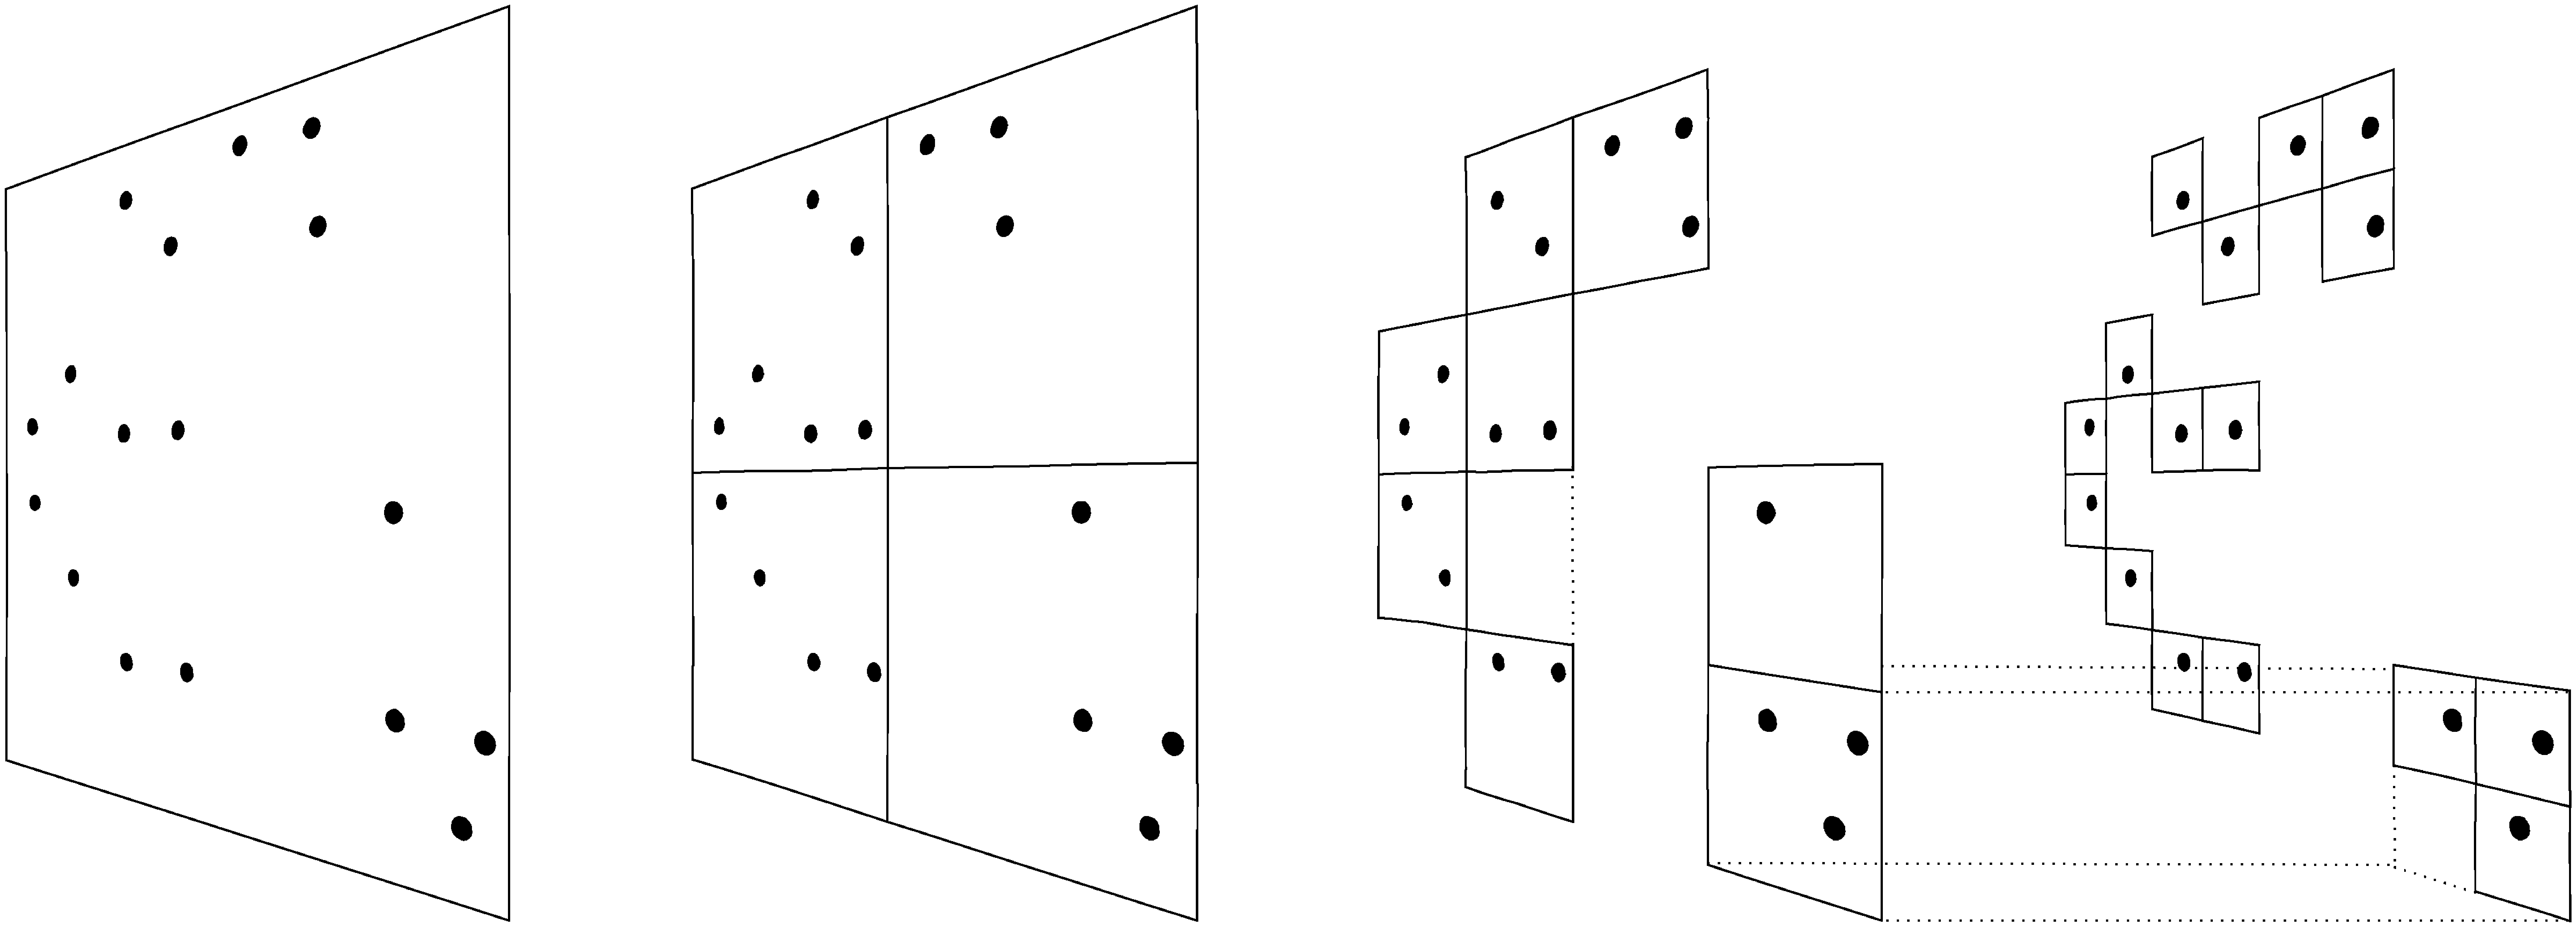
\includegraphics[width=\linewidth]{gadget/tree.eps}
	\caption[Barns-Hut oct-tree in two dimensions.]{Barns-Hut oct-tree in two dimensions.}
	\label{fig:gadget--tree}
\end{figure}



%:::::::::::::::::::::::::::::::::::::::::::::::::::::::::::::::::::::::::::::::
\subsubsection{Parallelization}
\label{subsubsec:gadget--gadget--parallelization}
%:::::::::::::::::::::::::::::::::::::::::::::::::::::::::::::::::::::::::::::::


Text goes here.

\begin{figure}[t]
	\centering
	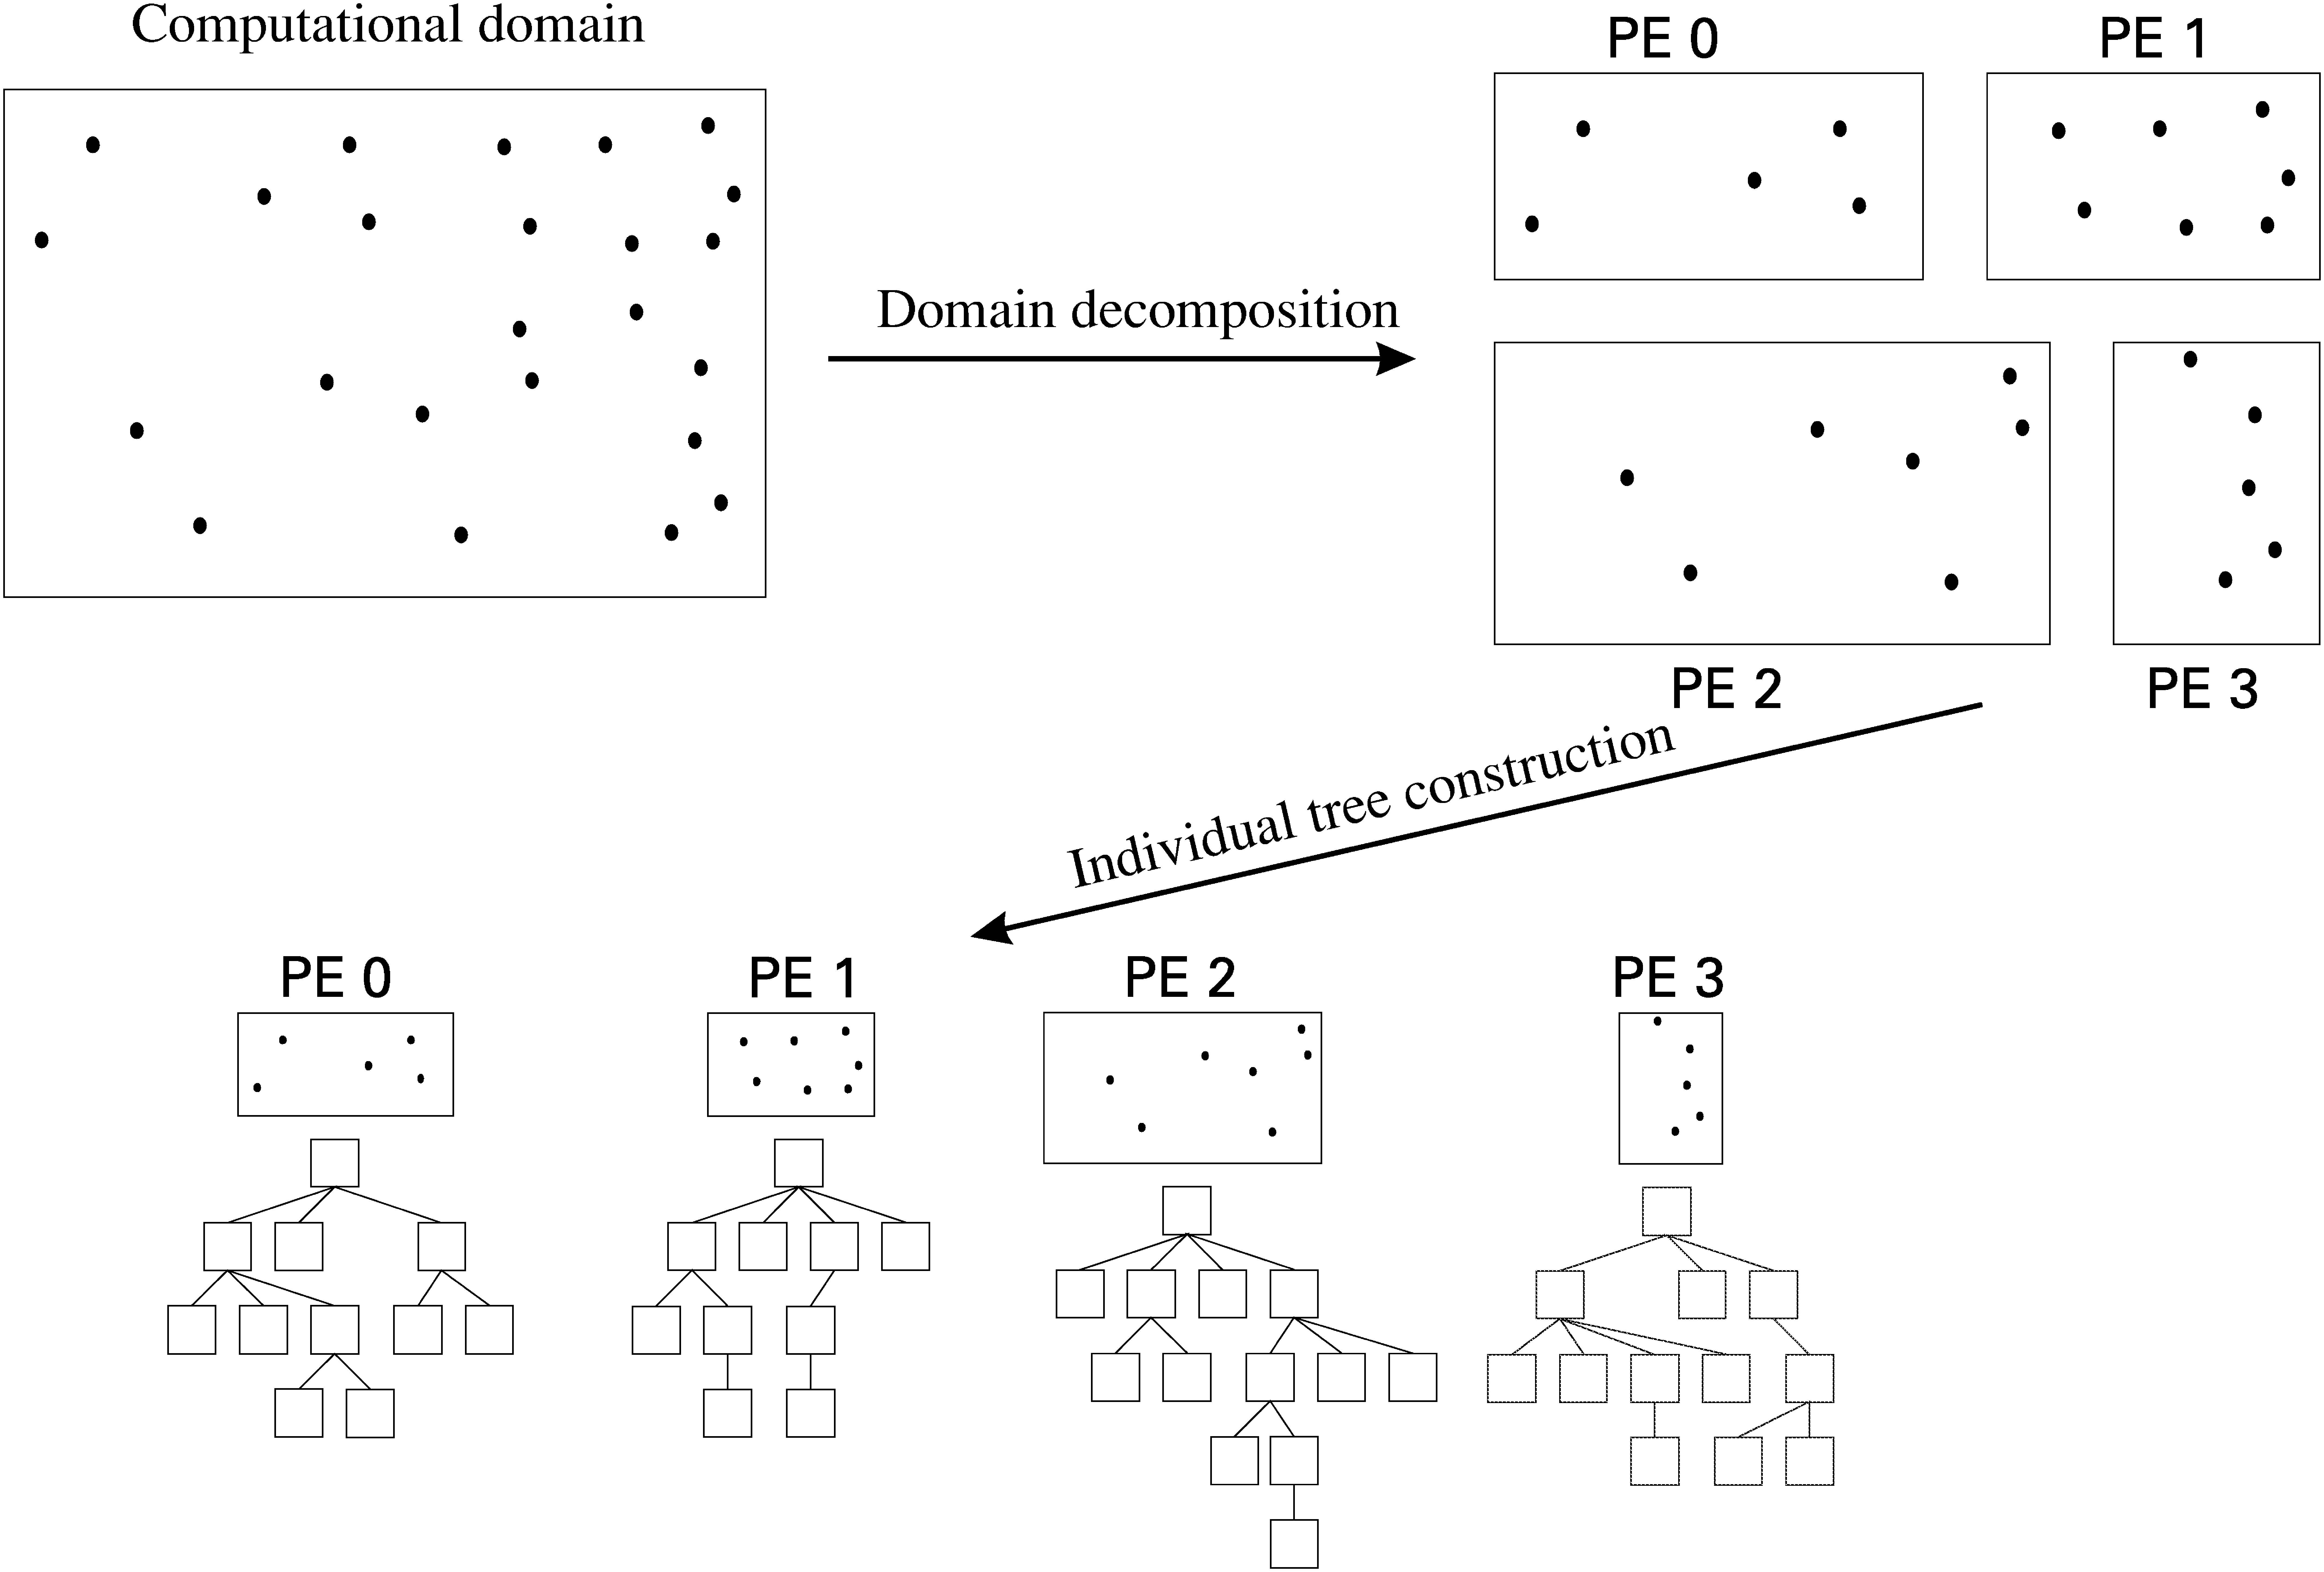
\includegraphics[width=\linewidth]{gadget/domain_decomp.eps}
	\caption[Domain decomposition.]{Domain decomposition.}
	\label{fig:gadget--domain_decomp}
\end{figure}

\begin{figure}[t]
	\centering
	
\includegraphics[width=\linewidth]{gadget/force_parallelism.eps}
	\caption[Force parallelism.]{Force parallelism.}
	\label{fig:gadget--force_parallelism}
\end{figure}



%:::::::::::::::::::::::::::::::::::::::::::::::::::::::::::::::::::::::::::::::
\subsubsection{Softening}
\label{subsubsec:gadget--gadget--softening}
%:::::::::::::::::::::::::::::::::::::::::::::::::::::::::::::::::::::::::::::::


Text goes here.

\begin{figure}[t]
	\centering
	\begin{subfigure}{}
		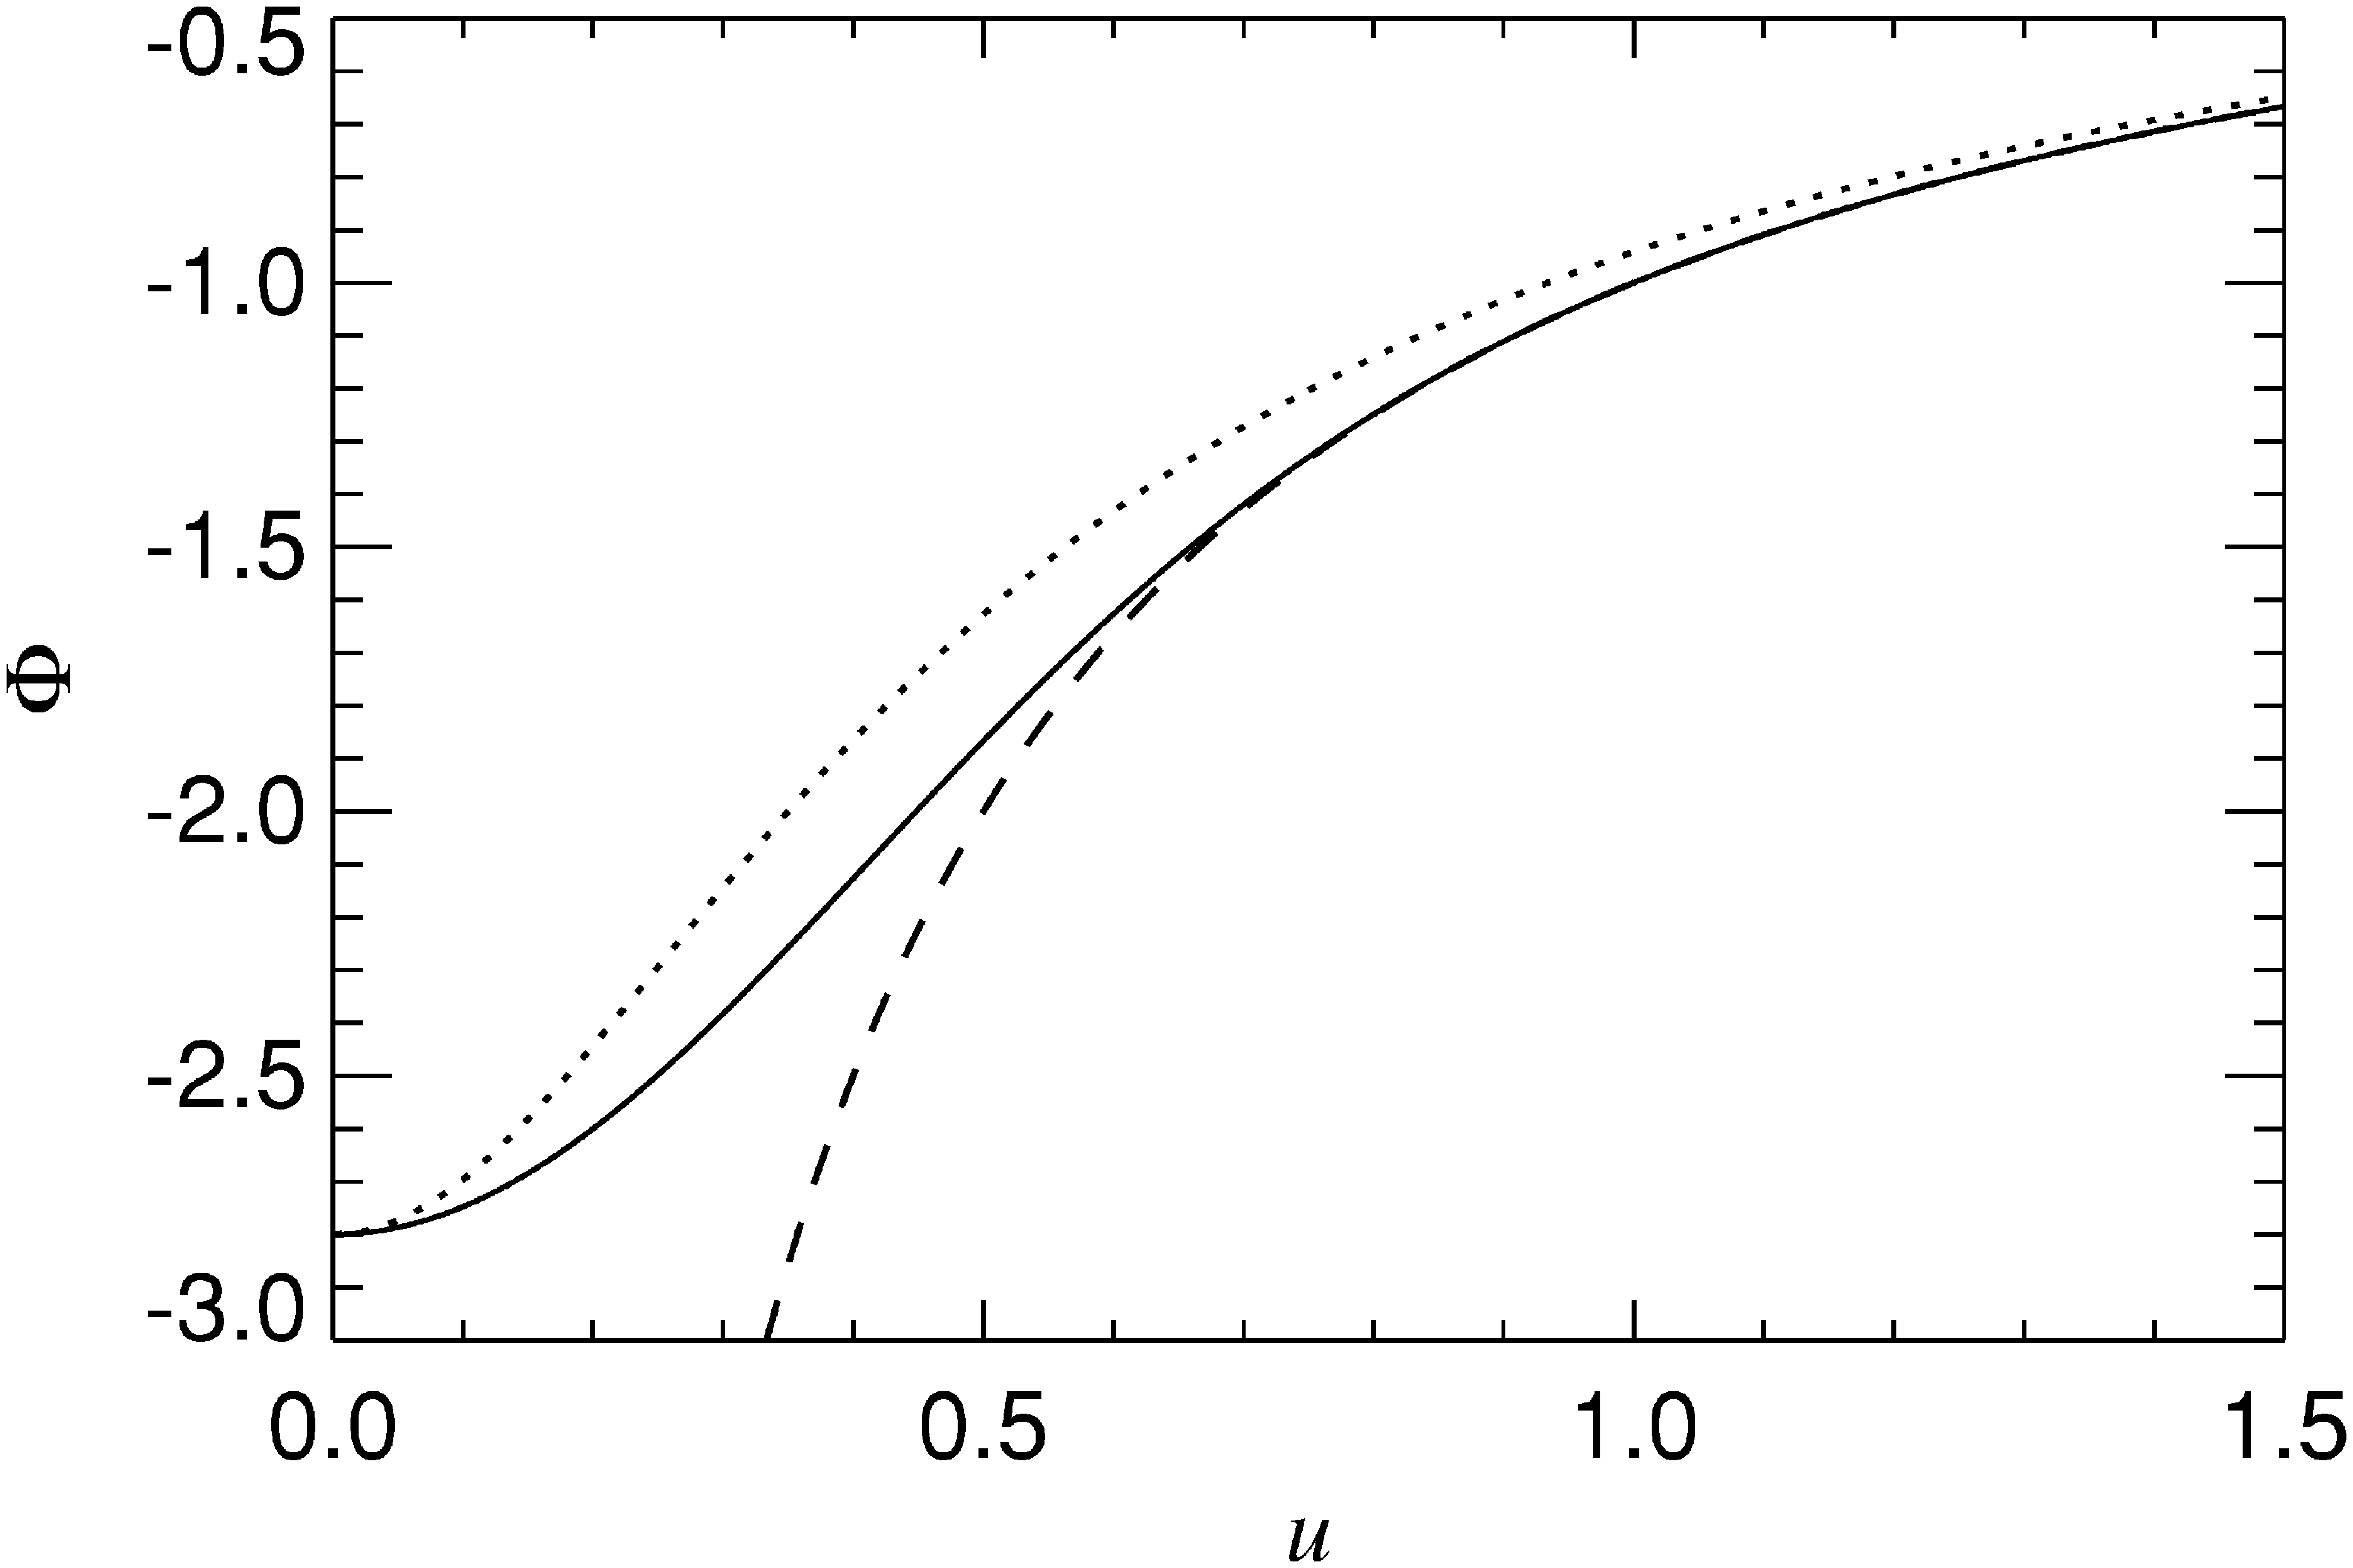
\includegraphics[width=0.45\linewidth]{gadget/softened_potential.eps}
	\end{subfigure}
	~
	\begin{subfigure}{}
		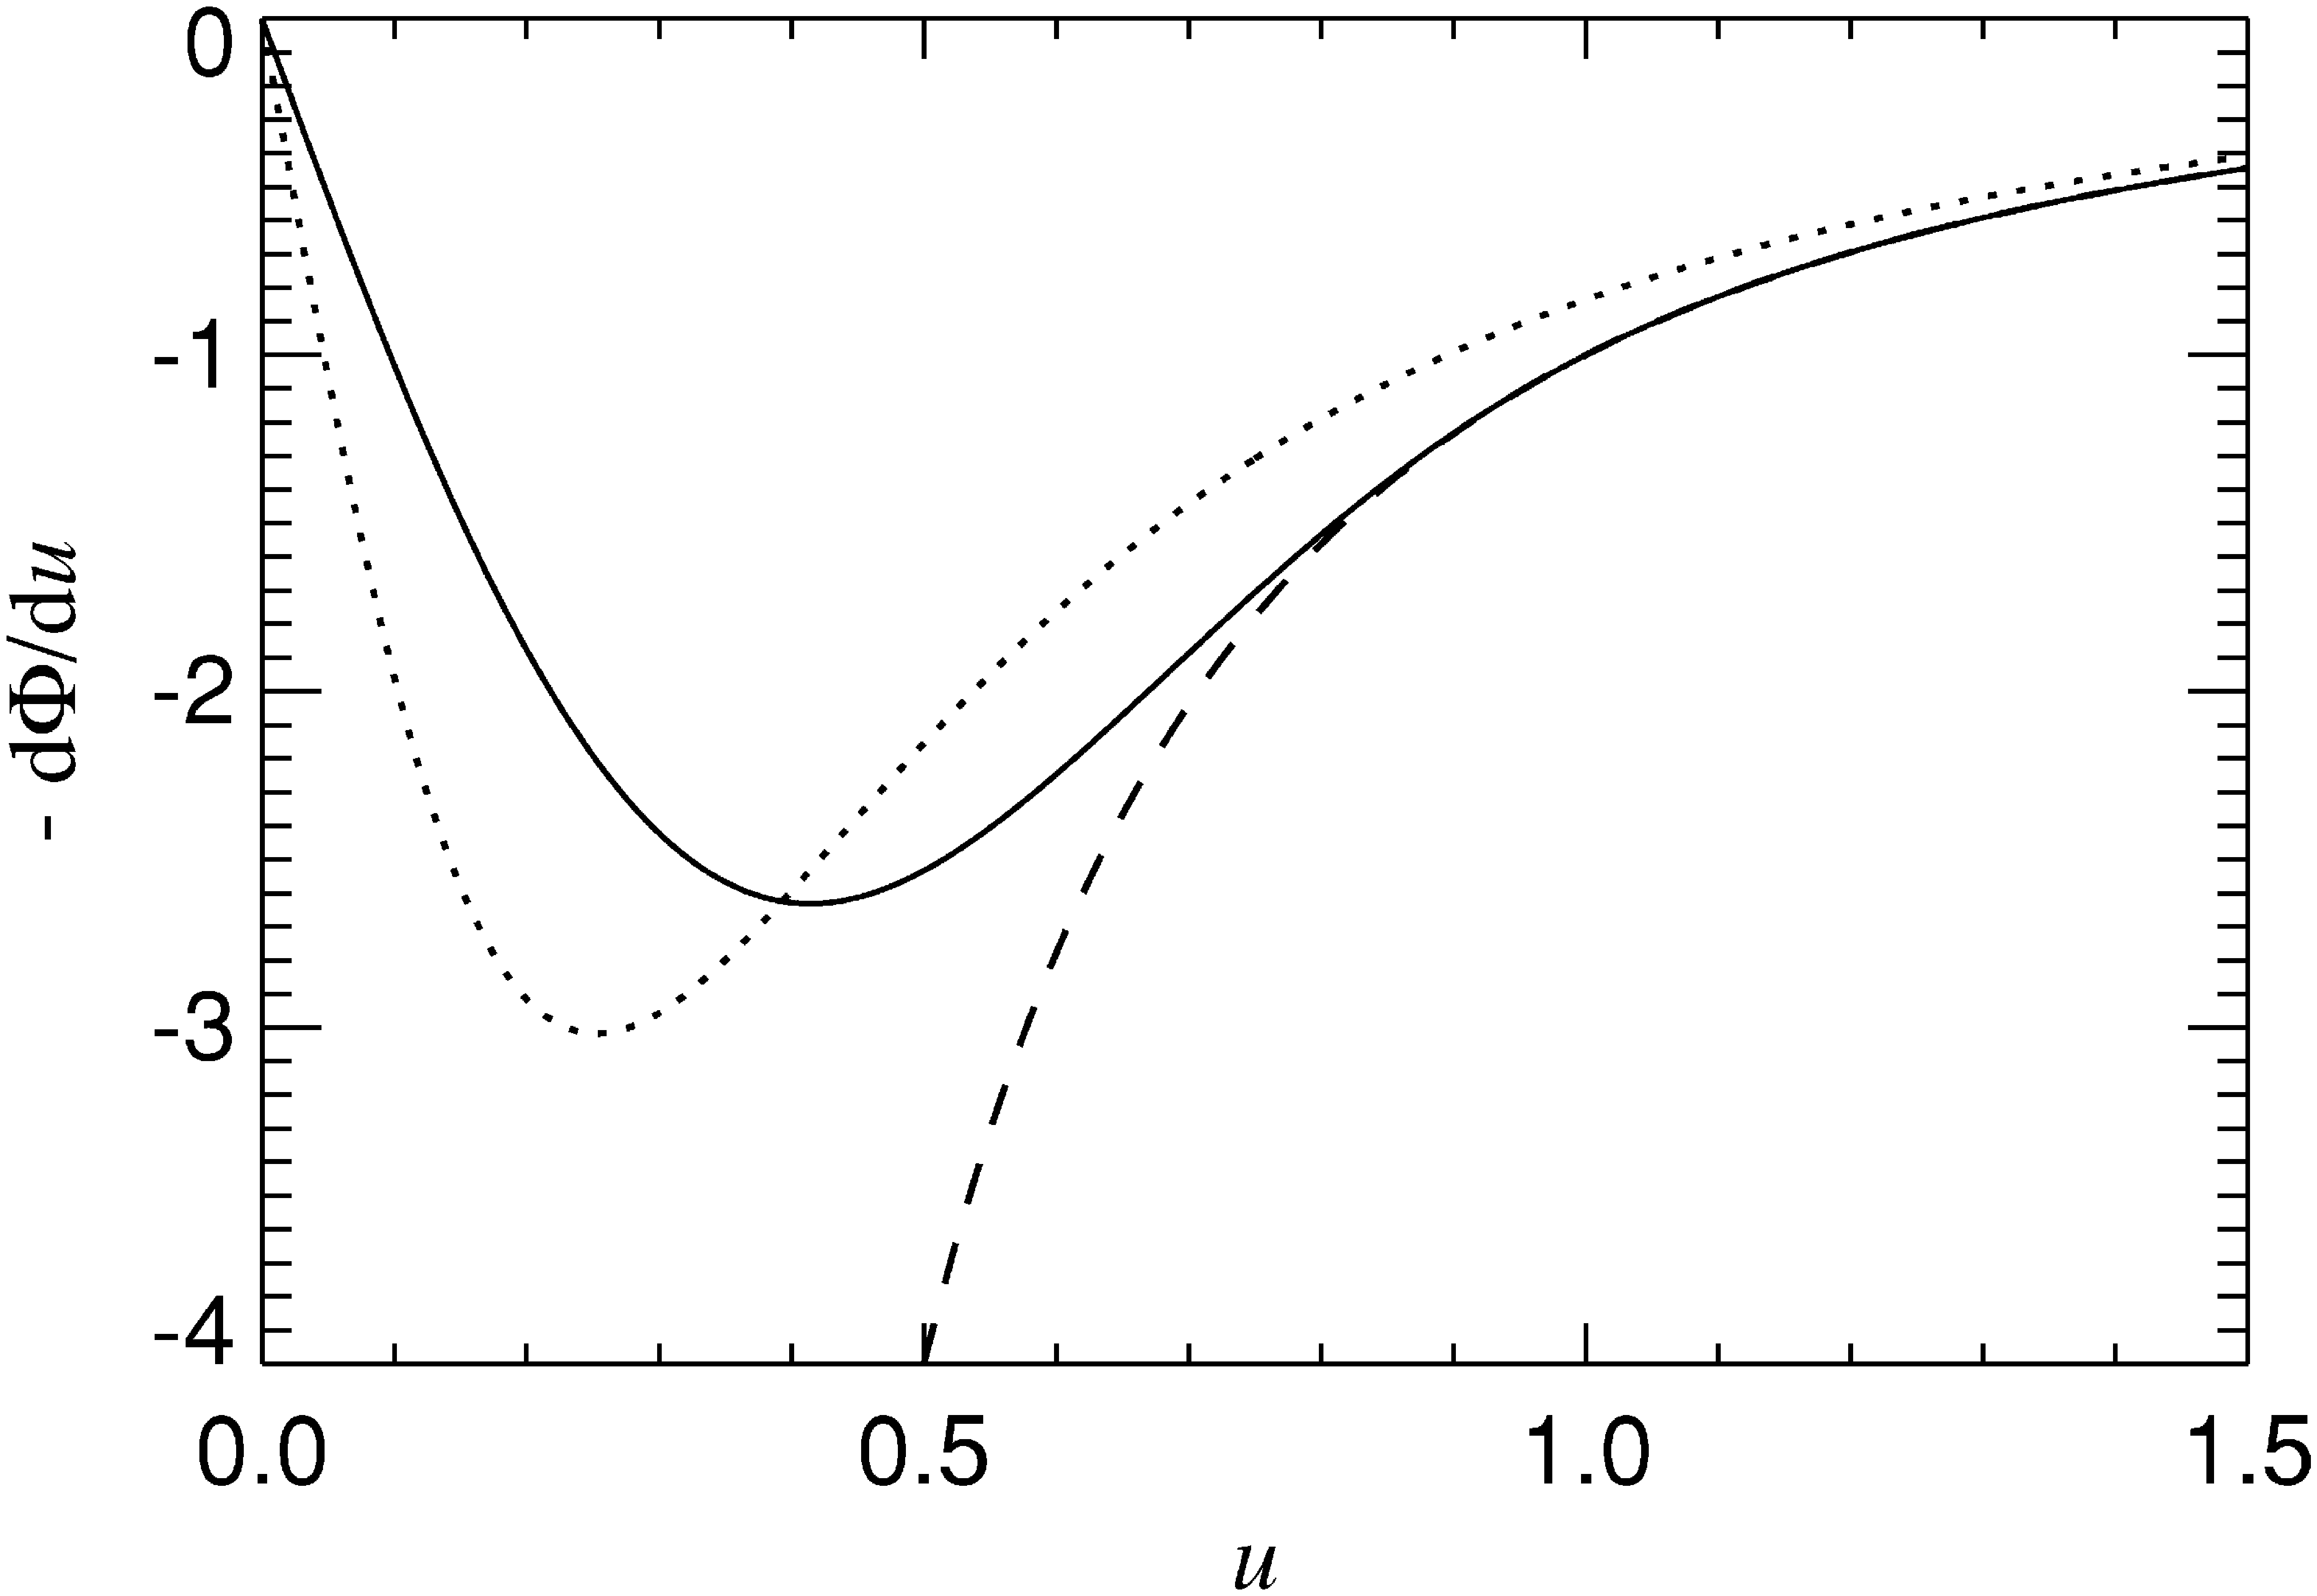
\includegraphics[width=0.45\linewidth]{gadget/softened_force.eps}
	\end{subfigure}
	\caption[Potential and force softening.]{Potential (\emph{left}) and force (\emph{right}) softening.}
	\label{fig:gadget--softening}
\end{figure}



%:::::::::::::::::::::::::::::::::::::::::::::::::::::::::::::::::::::::::::::::
\subsubsection{Metrics}
\label{subsubsec:gadget--gadget--metrics}
%:::::::::::::::::::::::::::::::::::::::::::::::::::::::::::::::::::::::::::::::


Text goes here.

\begin{figure}[t]
	\centering
	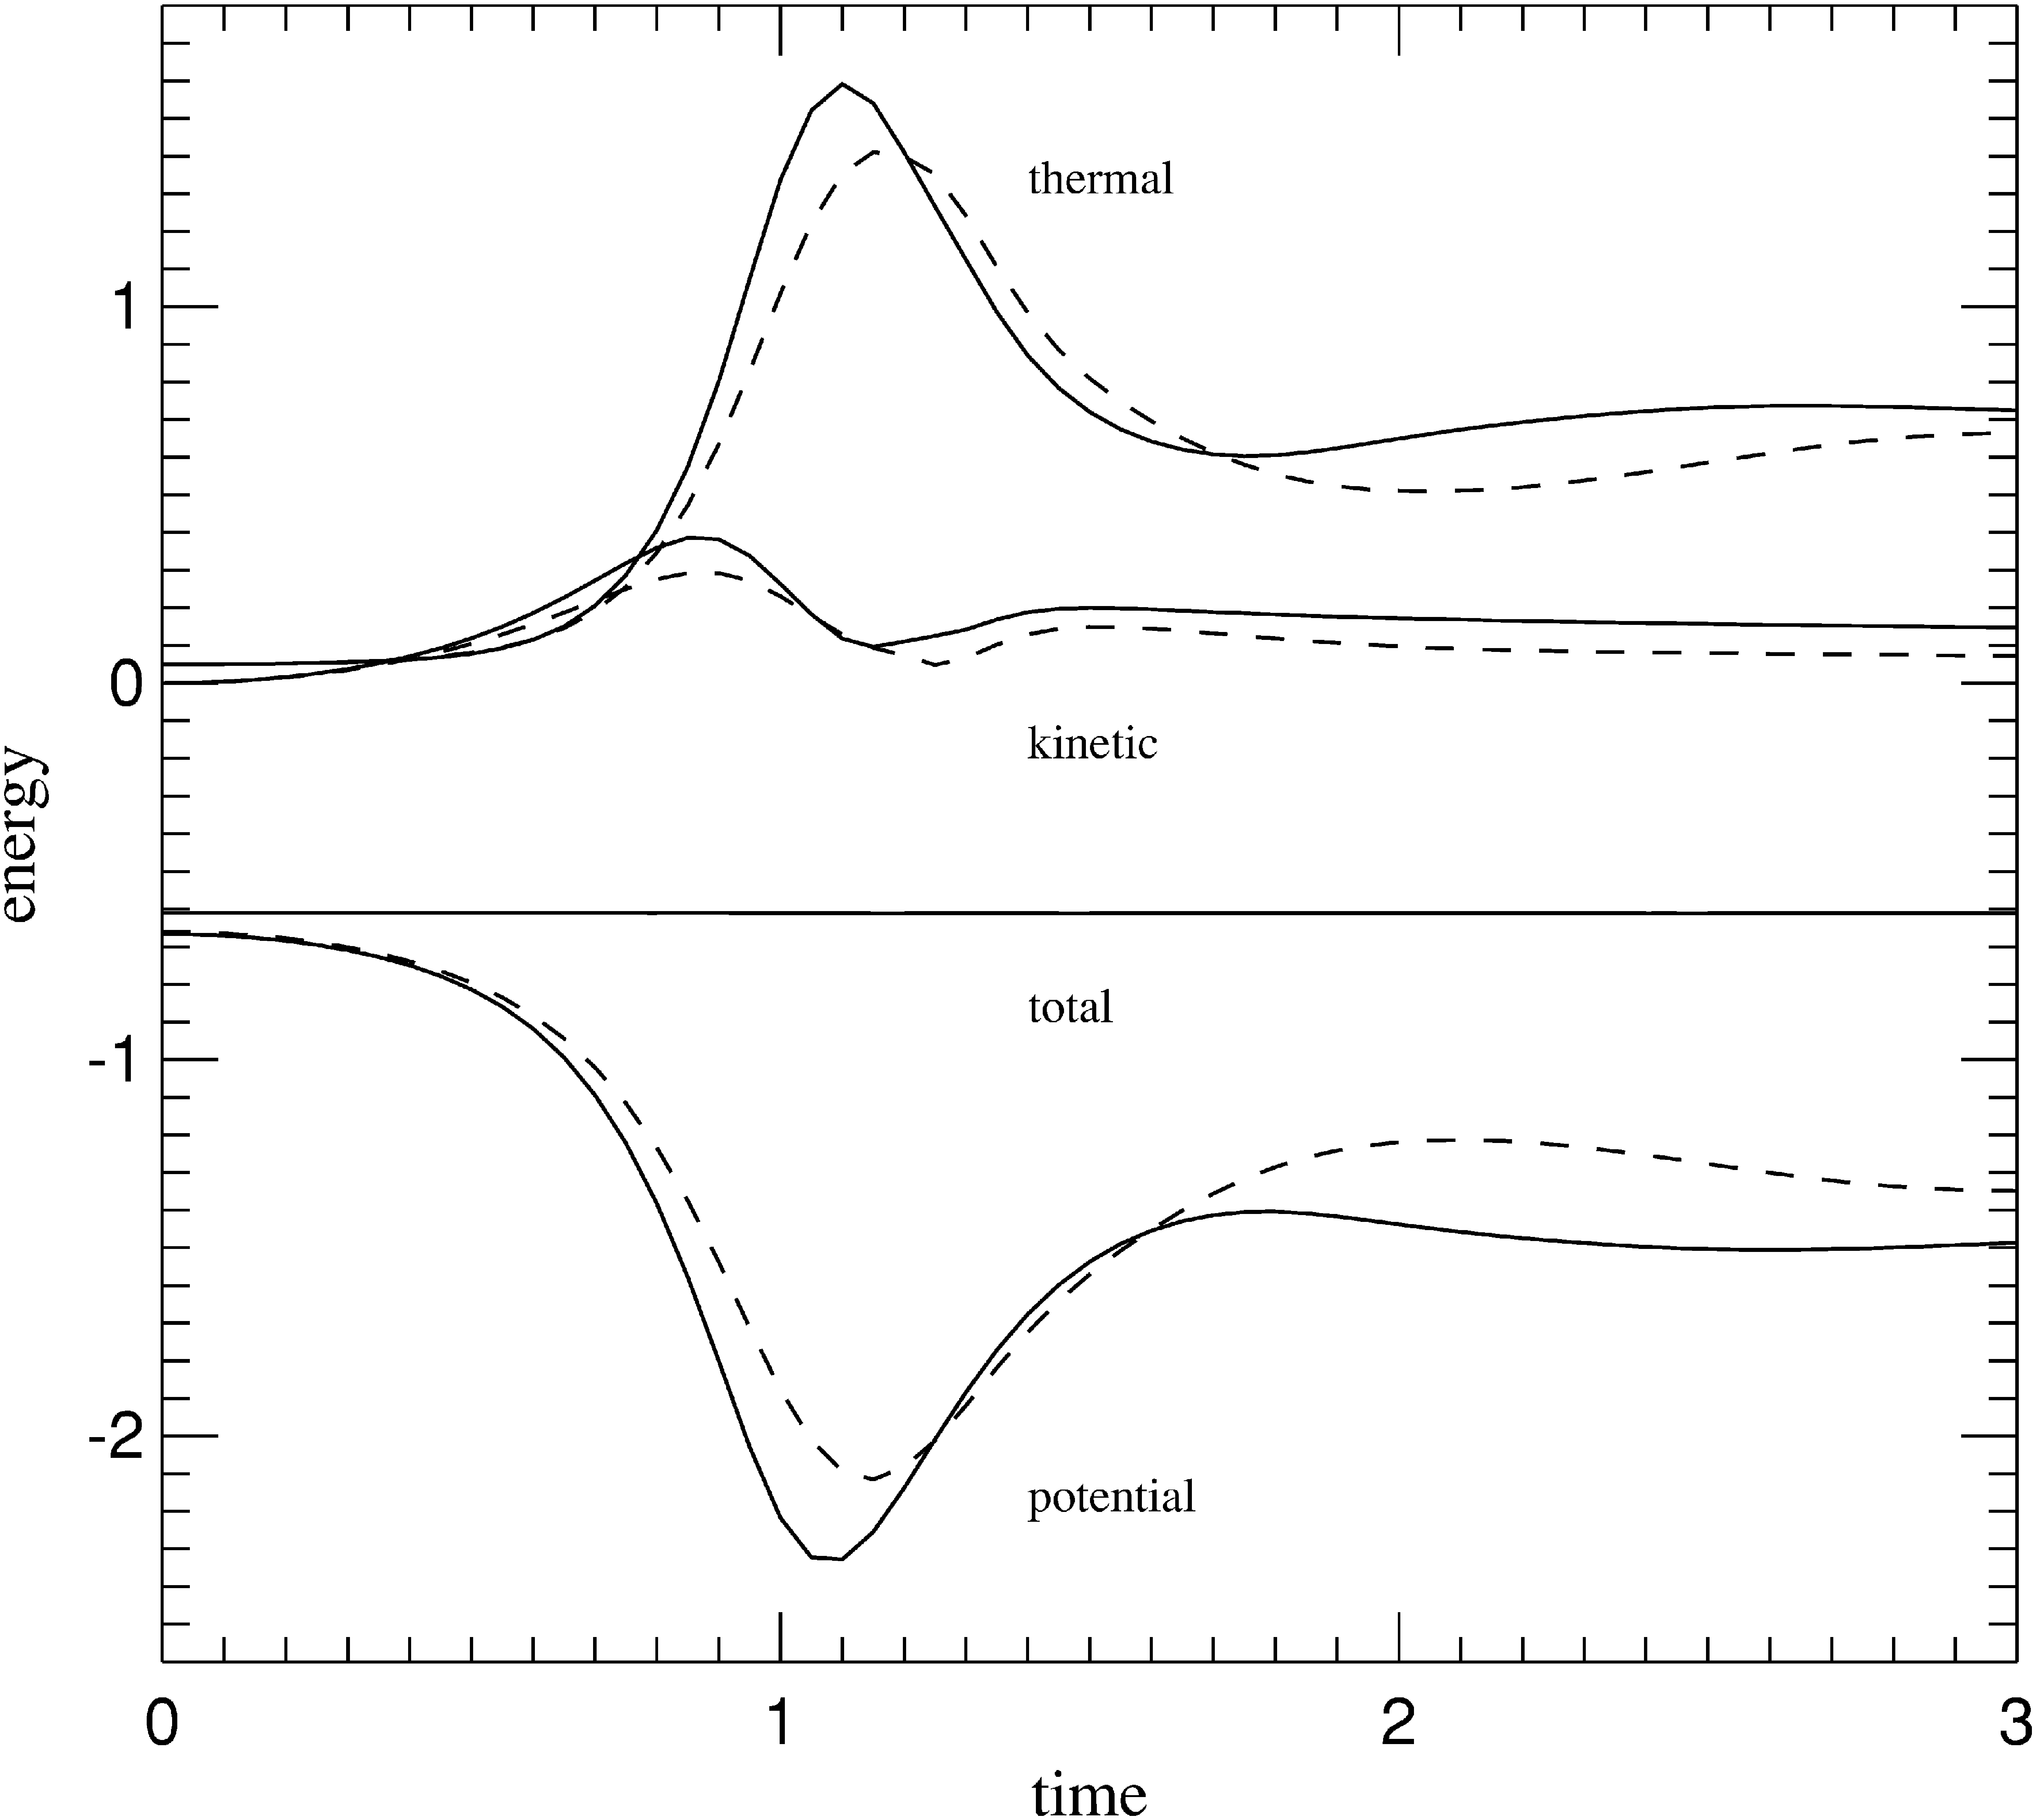
\includegraphics[width=0.75\linewidth]{gadget/energy_conservation.eps}
	\caption[Energy conservation for an initially isothermal gas sphere.]{Energy conservation for an initially isothermal gas sphere.}
	\label{fig:gadget--force_parallelism}
\end{figure}




%~~~~~~~~~~~~~~~~~~~~~~~~~~~~~~~~~~~~~~~~~~~~~~~~~~~~~~~~~~~~~~~~~~~~~~~~~~~~~~~
\subsection{Enhancements with \gadgettwo}
\label{subsec:gadget--subsection2}
%~~~~~~~~~~~~~~~~~~~~~~~~~~~~~~~~~~~~~~~~~~~~~~~~~~~~~~~~~~~~~~~~~~~~~~~~~~~~~~~


Text goes here.




%~~~~~~~~~~~~~~~~~~~~~~~~~~~~~~~~~~~~~~~~~~~~~~~~~~~~~~~~~~~~~~~~~~~~~~~~~~~~~~~
\subsection{Simulations}
\label{subsec:gadget--simulations}
%~~~~~~~~~~~~~~~~~~~~~~~~~~~~~~~~~~~~~~~~~~~~~~~~~~~~~~~~~~~~~~~~~~~~~~~~~~~~~~~


Text goes here.






%%%%%%%%%%%%%%%%%%%%%%%%%%%%%%%%%%%%%%%%%%%%%%%%%%%%%%%%%%%%%%%%%%%%%%%%%%%%%%%%
%
% Rockstar
%
%%%%%%%%%%%%%%%%%%%%%%%%%%%%%%%%%%%%%%%%%%%%%%%%%%%%%%%%%%%%%%%%%%%%%%%%%%%%%%%%

\section{Halo Finding with \rockstar}
\label{sec:rockstar}

%%%%%%%%%%%%%%%%%%%%%%%%%%%%%%%%%%%%%%%%%%%%%%%%%%%%%%%%%%%%%%%%%%%%%%%%%%%%%%%%


\rockstar\ \citep[Robust Overdensity Calculation using K-Space Topoloogically Adaptive Refinement; ][]{2013ApJ...762..109B} is a halo finder based on the hierarchical refinement of friends-of-friends (FOF) groups in six phase space dimensions and, optionally, one time dimensions.  It has been shown \citep{2011MNRAS.415.2293K} to be robust in recovering halo properties, determining substructure, and providing accurate particle member lists, even for notoriously difficult scenarios such as for low particle count halos and halos undergoing major merger events.




%~~~~~~~~~~~~~~~~~~~~~~~~~~~~~~~~~~~~~~~~~~~~~~~~~~~~~~~~~~~~~~~~~~~~~~~~~~~~~~~
\subsection{Halo Finding}
\label{subsec:rockstar--halo_finding}
%~~~~~~~~~~~~~~~~~~~~~~~~~~~~~~~~~~~~~~~~~~~~~~~~~~~~~~~~~~~~~~~~~~~~~~~~~~~~~~~


Halo finding in \rockstar\ is broken down into a number of steps, leading from the particle distribution of a simulation snapshot to the recovery of individual halo properties.  FOF overdensity groups are distributed among the analysis processors which build hierarchies of FOF subgroups in phase space, determine particle membership for halos, compute host halo/subhalo relationships, remove unbounded particles, and compute halo properties.  A summary of each of these steps is provided below.



%:::::::::::::::::::::::::::::::::::::::::::::::::::::::::::::::::::::::::::::::
\subsubsection{FOF Groups}
\label{subsubsec:rockstar--halo_finding--fof_groups}
%:::::::::::::::::::::::::::::::::::::::::::::::::::::::::::::::::::::::::::::::


The 3D friends-of-friends algorithm groups particles together if they fall within a set linking length of each other.  The linking length is often chosen as a fraction $b$ of the mean interparticle distance, with typical values ranging from $b = 0.15$ to $b = 0.2$ \citep{2011ApJS..195....4M}.  As \rockstar\ only uses FOF groups for breaking up the simulation volume to be distributed to individual processors, it is able use a modified algorithm for calculating FOF groups that is an order of magnitude faster than the typical procedure of finding all particles within the linking length for every particle.  For particles with more than 16 neighbor particles, the neighbor finding process is skipped for the neighboring particles.  Instead, particles are linked to the same group if they are within two linking lengths of the original particle.  This method runs much faster than the standard FOF algorithm, and links together at minimum the same particles.  With this approach, run time decreases instead of increases with increasing linking length.  \rockstar\ therefore uses a large linking length of $b = 0.28$.  The FOF groups are distributed among the available processors according to individual processor load.



%:::::::::::::::::::::::::::::::::::::::::::::::::::::::::::::::::::::::::::::::
\subsubsection{Phase-Space FOF Hierarchy}
\label{subsubsec:rockstar--halo_finding--phase_space}
%:::::::::::::::::::::::::::::::::::::::::::::::::::::::::::::::::::::::::::::::


Within each FOF group, FOF subgroups are found hierarchically in phase-space.  A phase-space linking length is adaptively chosen so that a constant fraction $f$ of particles are linked together with at least one other particle.  For two particles $p_{1}$ and $p_{2}$, the phase-space distance metric is defined as \citep{1998lsst.conf...43G}
\begin{equation}
	d(p_{1}, p_{2}) = \left( \frac{\left| \vec{x_{1}} - \vec{x_{2}} \right|^{2}}{\sigma_{x}^{2}} + \frac{\left| \vec{v_{1}} - \vec{v_{2}} \right|^{2}}{\sigma_{v}^{2}} \right)^{1/2},
\end{equation}
where $\sigma_{x}$ and $\sigma_{v}$ are the particle position and velocity dispersions for the FOF group.  The phase-space distance to the nearest neighbor is computed for each particle, the linking length is chosen such that $f = 0.7$, and a new FOF subgroup is determined.  This process is repeated recursively on the new FOF subgroups until a minimum threshold of 10 particles is reached at the deepest level of the hierarchy.



%:::::::::::::::::::::::::::::::::::::::::::::::::::::::::::::::::::::::::::::::
\subsubsection{Converting FOF Subgroups to Halos}
\label{subsubsec:rockstar--halo_finding--fof_to_halos}
%:::::::::::::::::::::::::::::::::::::::::::::::::::::::::::::::::::::::::::::::


Seed halos are created for each of the deepest level subgroups in the FOF hierarchy.  Particles from successively higher levels of the hierarchy are then assigned to the seed halos until all particles in the original FOF group are accounted for.  To suppress extraneous seed halo generation due to noise, seed halos are merged if their positions and velocities are within $10 \sigma$ of Poisson uncertainties of each.  Specifically, the halos are merged if
\begin{equation}
	\sqrt{(x_{1} - x_{2})^{2} \mu_{x}^{-2} + (v_{1} - v_{2})^{2} \mu_{v}^{-2}} < 10 \sqrt{2},
\end{equation}
with
\begin{equation}
	\mu_{x} = \sigma_{x} / \sqrt{n},
\end{equation}
\begin{equation}
	\mu_{v} = \sigma_{v} / \sqrt{n},
\end{equation}
where $\sigma_{x}$ and $\sigma_{v}$ are the position and velocity dispersions of the smaller seed halo, and $n$ is the number of particles of the smaller seed halo.

If a parent FOF group contains multiple seed halos, particles are assigned to the closest seed halo in phase space.  The distance between a halo $h$ and a particle $p$ is given by
\begin{equation} \label{eq:rockstar--halo_phase_space_distance}
	d(h,p) = \left( \frac{\left| \vec{x_{h}} - \vec{x_{p}} \right|^{2}}{r_{\mathrm{dyn, vir}}^{2}} + \frac{\left| \vec{v_{h}} - \vec{v_{p}} \right|^{2}}{\sigma_{v}^{2}} \right)^{1/2},
\end{equation}
\begin{equation}
	r_{\mathrm{dyn, vir}} = v_{\max} t_{\mathrm{dyn, vir}} = \frac{v_{\max}}{\sqrt{\frac{4}{3} \pi G \rho_{\mathrm{vir}}}},
\end{equation}
where the seed halo currently has velocity dispersion $\sigma_{v}$ and maximum circular velocity $v_{\max}$.  Here, ``vir'' refers to the virial overdensity as defined by \citet{1998ApJ...495...80B} for $\rho_{\mathrm{vir}}$, which is 360 times the background density at $z = 0$.  \rockstar\ does, however, allow other choices for density definitions.



%:::::::::::::::::::::::::::::::::::::::::::::::::::::::::::::::::::::::::::::::
\subsubsection{Substructure}
\label{subsubsec:rockstar--halo_finding--substructure}
%:::::::::::::::::::::::::::::::::::::::::::::::::::::::::::::::::::::::::::::::


Satellite membership is assigned based on phase-space distances before calculating halo masses.  Equation~\ref{eq:rockstar--halo_phase_space_distance} is used to find the distance to all other halos with a greater number of particles, treating each halo center as a particle.  The halo is then assigned to be a subhalo of the closest larger halo within the same FOF group, if one exists.  If data from an earlier time-step is available, then halo cores at the current time-step are linked to halos from the previous time-step based on the largest contribution to the current halo core's particle membership.

Halo masses are then determined so that particles assigned to the host are not counted in the mass of the subhalo, but particles in the subhalo are included in the mass of the host.  Subhalo membership is then recalculated such that subhalos are those that fall within $r_{\Delta}$ of more massive host halos.




%~~~~~~~~~~~~~~~~~~~~~~~~~~~~~~~~~~~~~~~~~~~~~~~~~~~~~~~~~~~~~~~~~~~~~~~~~~~~~~~
\subsection{Halo Properties}
\label{subsec:rockstar--halo_properties}
%~~~~~~~~~~~~~~~~~~~~~~~~~~~~~~~~~~~~~~~~~~~~~~~~~~~~~~~~~~~~~~~~~~~~~~~~~~~~~~~


Halo positions based on maximum density peaks are more accurate than those found by averaging all FOF halo particles \citep{2011MNRAS.415.2293K}.  As \rockstar\ has already determined the halo density distribution when calculating the FOF subgroup hierarchy, halo positions are readily calculated by taking the average position of the particles in the inner subgroup which best minimizes the Poisson error.

The velocity of the halo core can be substantial offset from that of the halo bulk \citep{2013ApJ...762..109B}.  The velocity for the halo is calculated as the average velocity of the particles within the innermost 10\% of the halo radius, as the galaxy hosted by the halo should be most associated with the halo core.

Halo masses are calculated using the spherical overdensity (SO) out to various density thresholds, including the virial threshold of \citet{1998ApJ...495...80B} and density thresholds relative to the background density and the critical density.  Mass calculations include all particles from the substructure contained in the halo, and can optionally remove unbound particles.  As subhalo particles can be isolated from those of the host halo, mass calculations for substructure can also be obtained with spherical overdensities using only the particles belonging to the subhalo.

The scale radius $R_{s}$ is determined by dividing halo particles up into up to 50 radial equal-mass bins, with a minimum of 15 particles per bin, and fitting an NFW profile to the bins to find the maximum-likelihood fit.  The Klypin scale radius \citep{2011ApJ...740..102K}, which uses $v_{\max}$ and $\Mvir$ to calculate $R_{s}$, is also determined.

A number of other parameters are calculated, including the angular momentum, halo spin parameter \citep{1969ApJ...155..393P}, Bullock spin parameter \citep{2001ApJ...555..240B}, central position offset (defined as the distance between the halo density peak and the halo center of mass), central velocity offset (defined as the difference between the halo core velocity and the bulk velocity), ratio of kinetic to potential energy, and ellipsoidal shape parameters \citep{2011ApJS..197...30Z}.






%%%%%%%%%%%%%%%%%%%%%%%%%%%%%%%%%%%%%%%%%%%%%%%%%%%%%%%%%%%%%%%%%%%%%%%%%%%%%%%%
%
% CrossMatch
%
%%%%%%%%%%%%%%%%%%%%%%%%%%%%%%%%%%%%%%%%%%%%%%%%%%%%%%%%%%%%%%%%%%%%%%%%%%%%%%%%

\section{\crossmatch}
\label{sec:crossmatch}

%%%%%%%%%%%%%%%%%%%%%%%%%%%%%%%%%%%%%%%%%%%%%%%%%%%%%%%%%%%%%%%%%%%%%%%%%%%%%%%%


Text goes here.






%%%%%%%%%%%%%%%%%%%%%%%%%%%%%%%%%%%%%%%%%%%%%%%%%%%%%%%%%%%%%%%%%%%%%%%%%%%%%%%%
%
% Analysis and Plotting
%
%%%%%%%%%%%%%%%%%%%%%%%%%%%%%%%%%%%%%%%%%%%%%%%%%%%%%%%%%%%%%%%%%%%%%%%%%%%%%%%%

\section{Analysis}
\label{sec:analysis}

%%%%%%%%%%%%%%%%%%%%%%%%%%%%%%%%%%%%%%%%%%%%%%%%%%%%%%%%%%%%%%%%%%%%%%%%%%%%%%%%


In this section, we discuss the details of the pipeline used for this work, including the analysis and plotting codes, databases, and automation scripts.  We also present an overview of the results obtained at each step.  A more in depth discussion of the observed trends and interpretations of results are presented in Sections~\ref{sec:2lpt--results} and \ref{sec:2lpt--discussion}, and the figures presented here are provided only as examples of the output of the analysis code.

As a high-level overview, we gather snapshots from previously run \lpt\ and \za\ simulations, find halos in each snapshot with \rockstar, match halos between simulations with \crossmatch, and compare the differences in various properties between corresponding \lpt\ and \za\ halos, primarily as functions of redshift and halo mass.  The specific codes developed for and used in our analysis are provided in the Appendices, and are referenced with the relevant discussions below.




%~~~~~~~~~~~~~~~~~~~~~~~~~~~~~~~~~~~~~~~~~~~~~~~~~~~~~~~~~~~~~~~~~~~~~~~~~~~~~~~
\subsection{Halo Properties with \rockstar}
\label{subsec:analysis--halo_properties}
%~~~~~~~~~~~~~~~~~~~~~~~~~~~~~~~~~~~~~~~~~~~~~~~~~~~~~~~~~~~~~~~~~~~~~~~~~~~~~~~


Halos are identified and measured with the \rockstar\ halo finder, which is discussed in detail in Section~\ref{sec:rockstar}.  Here, we discuss the setup necessary to run \rockstar, as well as its output files, post-processing steps, and particle list extraction.



%:::::::::::::::::::::::::::::::::::::::::::::::::::::::::::::::::::::::::::::::
\subsubsection{Simulation Snapshots and \rockstar\ Setup}
\label{subsubsec:analysis--halo_properties--setup}
%:::::::::::::::::::::::::::::::::::::::::::::::::::::::::::::::::::::::::::::::


We run \rockstar\ on snapshots from each of our six simulation boxes.  Each box has 62 snapshots, with $512^{3}$ dark matter particles each.  For each snapshot, a \rockstar\ run directory is set up with a number of configuration files and scripts, including the \rockstar\ configuration file (Appendix~\ref{app:onenode}), PBS submission script (Appendix~\ref{app:run_rockstar}), a script to clean files from previous runs and begin a new run (Appendix~\ref{app:begin_run}), and a script for post-processing generated output files (Appendix~\ref{app:postprocess}).  A directory for particle data contains a link to the actual simulation snapshot and a file containing a list of snapshot files, which for our setup contains only one item.  A directory is also created for output halo data files.  We discuss automation of run directory setup and simultaneous launching of multiple \rockstar\ instances in Section~\ref{sec:automation}.

The parameter file controls various configuration options including simulation type, physical units, cosmological parameters, I/O options, halo definitions, and process setup.  \rockstar\ has native support for \gadget's snapshot format and can automatically import cosmological parameters and box size.  Length and mass scales must be input to convert from simulation units.  \rockstar\ uses periodic boundary conditions based on the number of analysis processes.  Periodic boundary conditions are assumed if using a multiple of eight analysis processes and are not assumed if using one analysis process.  Halo virial radius and mass definitions may be set to either virial or a multiple of either the critical or background density.  We select halos to be defined by the virial radius and mass.  We are interested in defining halos as spherical overdensity halos rather than friends-of-friends halos, so we also choose to define halo properties based on all particles within the virial radius, whether or not they are energetically bound to the halo.

\rockstar\ is run as a server-client setup.  This is designed so that one processor acts as a director and output manager, one or more processors read in the input snapshots, and the remaining processors or compute nodes do the actual processing on different segments of the simulation box.  \rockstar\ uses sockets for communication between the server process and the worker processes if running on multiple nodes.  However, we run each instance of \rockstar\ on one node only, with ten processor cores for the necessary functions.  One processor acts as the server, one as the snapshot reader, and the remaining eight as halo finders.



%:::::::::::::::::::::::::::::::::::::::::::::::::::::::::::::::::::::::::::::::
\subsubsection{\rockstar\ Output and Post-processing}
\label{subsubsec:analysis--halo_properties--output}
%:::::::::::::::::::::::::::::::::::::::::::::::::::::::::::::::::::::::::::::::


\rockstar\ outputs halo information in ASCII plaintext, binary, and BGC2 binary formats.  As mentioned above, we run \rockstar\ with eight worker processes per snapshot.  Each worker process outputs its own set of data files, with each file covering a separate octant of the simulation box plus a small overlap region.  Halos with particles in the overlap region are saved based on the location of their centers.  In addition to the per-processor output, a composite list of halos (and only halos) from all worker processors are created.

Through its various output files, \rockstar\ provides a large number of measured halo properties, including halo ID, number of constituent particles, masses to various radii, position, velocity, angular momentum, spin, virial radius, scale radius, shape parameters, energy parameters, position and velocity offsets between the center of mass and the peak density, and parent halo ID.  Whether or not full friends-of-friends particle lists are saved is controlled via the configuration file.  In addition, spherical overdensity particle lists of particle positions, velocities, and IDs are saved only when utilizing BGC2 output.  Individual particle masses are not included as our simulations have uniform particle mass.

As previously mentioned, we want halos defined based on spherical overdensity particle lists.  These are only available from \rockstar's BGC2 binary output format, with all other available particle lists consisting of friends-of-friends particles.  The BGC2 files consist of a 1024 byte header, halo data of 72 bytes per halo, and particle data with 32 bytes per particle.  The header consists of an unsigned 8-byte integer, 16 8-byte signed integers, 19 8-byte double-precision floating point numbers, and extra padding out to 1024 bytes.  We refer the reader to the bgc2.h header file in the publicly available \rockstar\ source code for the list and explanation of the header variables.  The data for each halo consist of 2 8-byte signed integers for ID and parent ID, 2 8-byte unsigned integers for number of particles and number of particles excluding substructure, and 10 4-byte floating point numbers for radius, mass, three position components, three velocity components, maximum circular velocity, and the radius of the maximum circular velocity.  The data for each particle consist of 1 8-byte signed integer for ID and 6 4-byte floating point numbers for three position components and three velocity components.  There is a 4-byte offset before the header, and 8-byte offsets between the header and halo data and between the halo data and particle data.  Our python code for reading in BGC2 files is presented in Appendix~\ref{app:bgc2}.  C code for reading in BGC2 files is bundled with the \rockstar\ source code.

After \rockstar\ is run, some post-processing of the output is needed.  By default, \rockstar\ does not provide information on membership information for substructure.  Two scripts---one for the composite halo list and one for the BGC2 files---are provided with \rockstar\ to cycle back through the halo lists and find the "parents," or the halo in which a given subhalo is contained.  A script is also provided to convert halo information in the BGC2 files to ASCII plaintext.  Our script for running these post-processing steps is presented in Appendix~\ref{app:postprocess}.




%~~~~~~~~~~~~~~~~~~~~~~~~~~~~~~~~~~~~~~~~~~~~~~~~~~~~~~~~~~~~~~~~~~~~~~~~~~~~~~~
\subsection{Density Profile Fitting}
\label{subsec:analysis--profile_fitting}
%~~~~~~~~~~~~~~~~~~~~~~~~~~~~~~~~~~~~~~~~~~~~~~~~~~~~~~~~~~~~~~~~~~~~~~~~~~~~~~~


While \rockstar's output includes measurements for halo virial and scale radii, and thus concentration, we independently fit NFW density profiles to halos and measure concentration as a verification of \rockstar's fitting.  The full density profile python code is presented in Appendix~\ref{app:density_profile}.  This section is included for completeness only, as we find that only a small fraction of halos are well fit by our method, and we instead rely on concentration measurements directly from \rockstar\ for subsequent analysis.



%:::::::::::::::::::::::::::::::::::::::::::::::::::::::::::::::::::::::::::::::
\subsubsection{Density Profiles}
\label{subsubsec:analysis--profile_fitting--density_profiles}
%:::::::::::::::::::::::::::::::::::::::::::::::::::::::::::::::::::::::::::::::


For each halo, a list of constituent spherical overdensity particles is obtained from the post-processed BGC2 catalog from \rockstar's output.  For our purposes here, the relevant parameters are particle mass and position.  We also use the values for each halo's center position and virial radius as found by \rockstar.

Density profiles are then constructed by binning the particle positions in logarithmic radial bins from the resolution limit of the simulation to the halo virial radius and multiplying by particle mass.  Before being passed to the fitting routine, density profiles are normalized to unity for both virial radius and maximum density. 



%:::::::::::::::::::::::::::::::::::::::::::::::::::::::::::::::::::::::::::::::
\subsubsection{Fitting}
\label{subsubsec:analysis--profile_fitting--fitting}
%:::::::::::::::::::::::::::::::::::::::::::::::::::::::::::::::::::::::::::::::


Halos are fit using the CurveFit routine from the SciPy Optimize library.  It uses the Levenberg-Marquardt algorithm \citep{1963SIAM...11...431} for non-linear least squares fitting.

CurveFit is called by providing a model function, independent variable, measured dependent variable, and optionally weights for the dependent variable and initial guesses for fit coefficients.  Here, our fit function is the NFW dark matter density profile (see Equation~\ref{eq:early_universe--nfw_profile}).  The free parameters to be fit are the scale radius $R_{s}$ and the characteristic density $\rho_{0}$.

As the least squares algorithm is sensitive to local minima, care must be taken in choosing initial guesses for the fit coefficients.  Additionally, large dynamic range in the fit parameters tended to produce poor results.  We explored a number of approaches to improve solution stability, including fitting in logarithmic space and randomizing the initial guesses and picking the best solution.  We found the best results were achieved by normalizing the data to unity for both radius and density, and choosing initial guesses within an order of magnitude for a typical halo, namely, normalized $R_{s} = 0.1$ and normalized $\rho_{0} = 1.0$.

Some halos with irregular profiles presented the problem of the fitting algorithm choosing an unphysical scale radius larger than the virial radius of the halo.  In order to heavily penalize this option from being chosen by the fitting algorithm, the fit density profile returned by the model function must differ from the input measured density profile as much as possible.  However, we discovered that the transition between a real fit and a purposefully distorted fit must also be smooth, as a disjointed jump such as, say, returning a very large number for every value if $R_{s} > R_{\mathrm{vir}}$ would cause the algorithm to fail.  We achieve this smooth transition penalty by adding the term $(R_{s} - 1) e^{r}$ to the density returned by the model function if the fitting algorithm tries to guess a value of $R_{s}$ larger than $R_{\mathrm{vir}}$.  However, while this did force halos to have definable concentrations, these halos often ended up with best fit scale radii equal to or just slightly less than the virial radii.

As we fit halos over a large range in redshift, we found low particle count halos to have noisy density profiles that were inherently more difficult to properly fit.  Throughout our analysis, we use a lower bound of 100 particles to define a halo.  At high redshift, even the largest halos are just beginning to cross this threshold.  With so few particles spread across the number of bins necessary to properly define a density profile (we adaptively reduce the number of bins if there are too few particles in a bin, with a minimum of 5 bins), we are left with only a handful of particles per bin.  In Figure~\ref{fig:fitting--density_profiles}, we compare one of the largest halos at $z = 14$ with one of the largest halos at the end of the simulation at $z = 6$.

\begin{figure}[tp]
	\centering
	\begin{subfigure}{}
		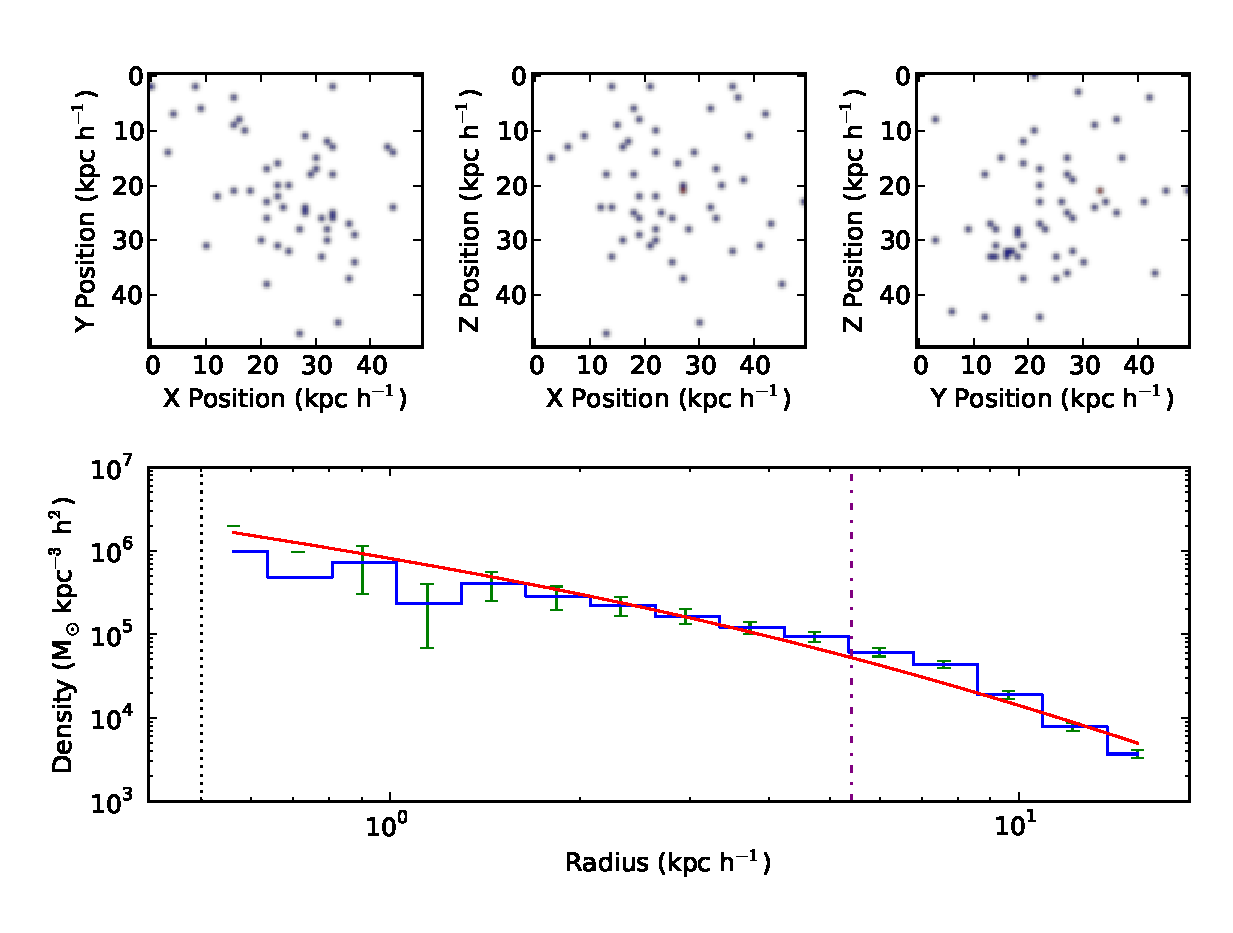
\includegraphics[width=0.75\linewidth]{analysis/2lpt_040_density_profile_0.eps}
	\end{subfigure}
	\\
	\begin{subfigure}{}
		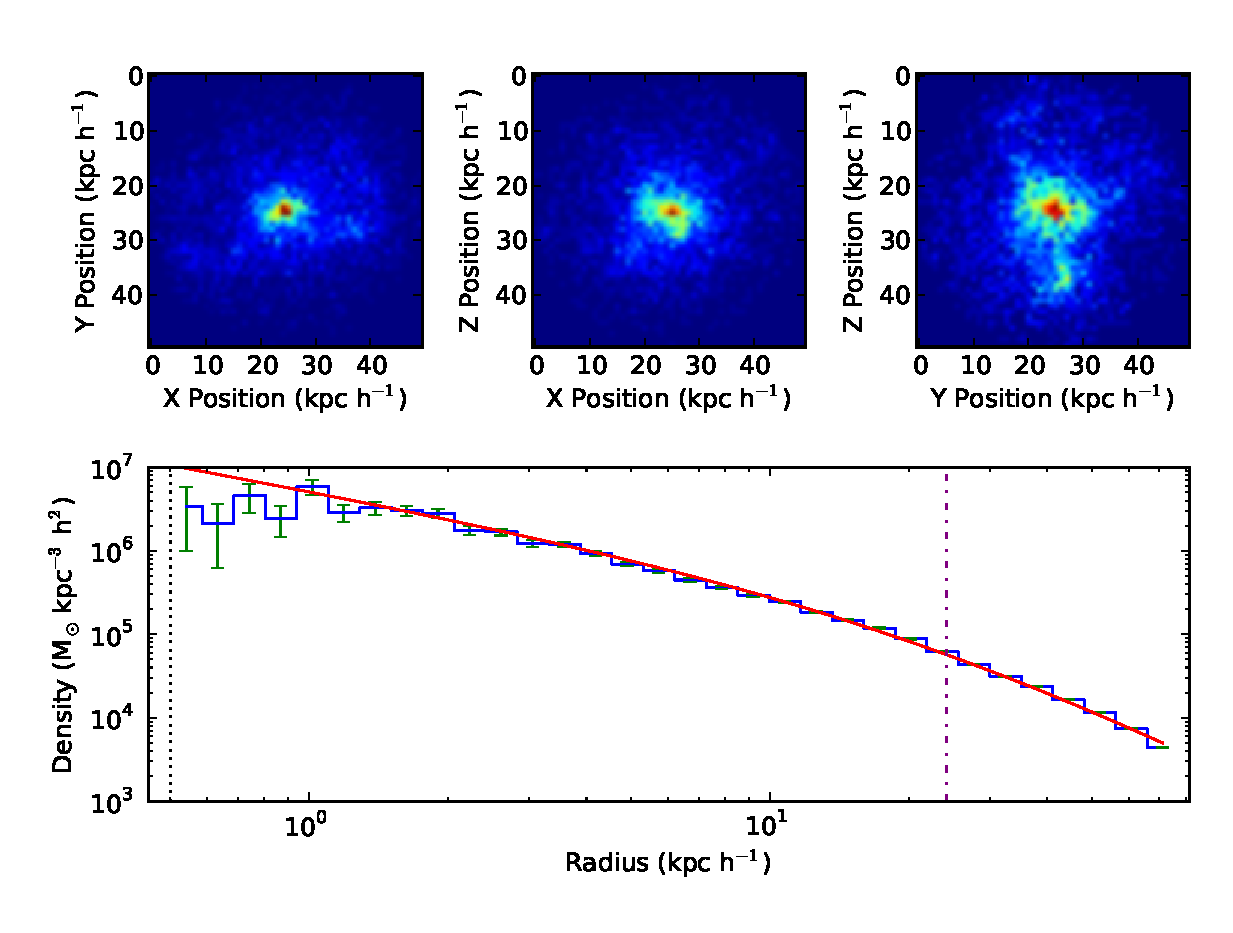
\includegraphics[width=0.75\linewidth]{analysis/2lpt_061_density_profile_0.eps}
	\end{subfigure}
	\caption[Density profiles for two large halos at $z = 14$ and $z = 6$.]{\footnotesize Spacial projections and density profiles for two large halos at $z = 14$ (\emph{top}) and $z = 6$ (\emph{bottom}).  Both halos are from the Box 1 \lpt\ simulation, and are the largest halos at their respective redshifts.  The density profiles are fit with an NFW profile, and the resulting scale radius is plotted as a vertical dot-dash purple line.}
	\label{fig:fitting--density_profiles}
\end{figure}



%:::::::::::::::::::::::::::::::::::::::::::::::::::::::::::::::::::::::::::::::
\subsubsection{Characterization of Uncertainty}
\label{subsubsec:analysis--profile_fitting--uncertainty}
%:::::::::::::::::::::::::::::::::::::::::::::::::::::::::::::::::::::::::::::::


An initial motivation for finding our own concentration parameters independent from \rockstar\ is that \rockstar\ does not provide information about the quality of its density profile fits.  We assign Poisson errors to the density in each bin such that $\sigma_{\rho} = \rho \sqrt{N} / N$, where $\rho$ is the density and $N$ is the number of particles in each bin.  These uncertainties are then provided as weights to the CurveFit routine.  Upon finding a best fit, the routine provides the fit parameters and an estimation of the uncertainty in those parameters via a covariance matrix, which we use to calculate the uncertainty in the concentration.  Additionally, we find the $\chi^{2}$ for the overall fit, which we use as an indicator of whether to accept or reject the fit for a given halo.  We accept halos with $\chi^{2} \le 10$.



%:::::::::::::::::::::::::::::::::::::::::::::::::::::::::::::::::::::::::::::::
\subsubsection{Concentration Comparison to \rockstar}
\label{subsubsec:analysis--profile_fitting--rockstar_comparison}
%:::::::::::::::::::::::::::::::::::::::::::::::::::::::::::::::::::::::::::::::


Overall, we do not find good agreement with \rockstar.  Using a script (see Appendix~\ref{app:concentration_comparison}) to compare the concentrations derived from our fits with those from \rockstar, we find that at $z = 6$ only 26\% of halos fit by our method have concentrations within 20\% of concentrations as measured by \rockstar.  We have slightly more agreement with high mass halos, with 37\% agreement if we only consider the most massive 10\% of halos.  Additionally, we do not find good fits for every halo.  If the distribution of particles would produce too few bins or the fitting routine exceeded a maximum number of iterations to find a stable solution, the halo is not fit.  We also exclude halos with fits returned with very large $\chi^{2}$ values.  Because of the discrepancies in our results and the fact that we do not find acceptable fits for every halo, we use the more complete \rockstar\ data for the final concentration measurements used in the remainder of our analysis.




%~~~~~~~~~~~~~~~~~~~~~~~~~~~~~~~~~~~~~~~~~~~~~~~~~~~~~~~~~~~~~~~~~~~~~~~~~~~~~~~
\subsection{Cross-matched Halo Catalog}
\label{subsec:analysis--catalog}
%~~~~~~~~~~~~~~~~~~~~~~~~~~~~~~~~~~~~~~~~~~~~~~~~~~~~~~~~~~~~~~~~~~~~~~~~~~~~~~~


We need to be able to directly compare corresponding halos from the two suites of simulations.  We match halos between \za\ and \lpt\ simulations based on constituent particles with the \crossmatch\ code modified to import \rockstar's BGC2 binary output files.  Properties of the matched halos are then compiled into one large database per box for further filtering and analysis.



%:::::::::::::::::::::::::::::::::::::::::::::::::::::::::::::::::::::::::::::::
\subsubsection{Cross-matching}
\label{subsubsec:analysis--catalog--crossmatching}
%:::::::::::::::::::::::::::::::::::::::::::::::::::::::::::::::::::::::::::::::


Our simulations are initialized with identical particle ID schemes, and we are thus able to uniquely identify and track matching particles between simulations and match halos based on the largest number of shared particles.  As the full implementation of the \crossmatch\ code is previously discussed in Section~\ref{sec:crossmatch}, we only briefly summarize its place in our analysis pipeline here.  The script in Appendix~\ref{app:crossmatch_setup} sets up the directory structure for the \crossmatch\ analysis and copies the \crossmatch\ parameter files (Appendices~\ref{app:crossmatch_2lpt_config} and \ref{app:crossmatch_za_config}) to the appropriate run directories.  \crossmatch\ is then run for each snapshot via the submission script in Appendix~\ref{app:run_crossmatch}, which is run for each simulation box.

Once caveat of the \crossmatch\ code is that matches are not necessarily unique.  For each halo in the first simulation, only one best match halo will be selected from the second simulation.  However, there may be other halos from the first simulation that also have the same halo from the second simulation selected as a best match.  For example, such a situation may arise in the case of offset merging epochs.  To counter this, we run \crossmatch\ in both directions---once matching \za\ halos to \lpt\ halos and once matching \lpt\ halos to \za\ halos---and choose best match halos as those that are matched in both directions.  This assures a unique one-to-one matching between \lpt\ and \za\ halos.  The code and submission script that select the best matches from the \lpt-first and \za-first cross-matched halo lists are presented in Appendix~\ref{app:crossmatch_best_match}.



%:::::::::::::::::::::::::::::::::::::::::::::::::::::::::::::::::::::::::::::::
\subsubsection{Database Aggregation and Filtering}
\label{subsubsec:analysis--catalog--aggregation}
%:::::::::::::::::::::::::::::::::::::::::::::::::::::::::::::::::::::::::::::::


We now have raw halo data we need for further study, but are also left with a large number of disparate files that contain this information.  For every snapshot, we have cross-simulation halo matching information from \crossmatch\ and the best match selection script, independent density profile and concentration measurement information from the density profile program, and original halo properties and host halo membership information from \rockstar\ spread across plaintext and BGC2 binary files for each processor on which \rockstar\ was run, all for three simulation boxes each for both \lpt\ and \za.

We combine the information from all of these file into one centralized database per snapshot with the database generation program and submission script in Appendix~\ref{app:database_generation}.  The program reads in all of the source data files, finds companion halos from the output of \crossmatch, and outputs all available data for each halo pair aggregated together.  The program is run for each of our 62 snapshots per simulation box, giving 186 total database files.

With the first version of our database generation code, total runtime became a significant factor.  The halo matching code was initially implemented in a naive double loop search through all the data files to find collect halo pair properties.  Pure python loop structures are exceedingly slow for larger data sets, and an initial estimate gave a runtime on the order of weeks or months.  This was unacceptable, as there are many snapshots, and the aggregation may need to be performed multiple times if any of the previous steps in the analysis pipeline were to be modified.  The code was therefore rewritten to take full advantage of the vectorization of the NumPy library, achieving a massive speedup to a runtime of order a few seconds.

In order to retain a centralized database of all available information for matched halos, we do not filter out halos at this step.  Subsequent analysis, however, does remove halo pairs from consideration in certain circumstances.  For early analysis involving our independent density profile fitting, we ignore halos based on evidence of a poor fit, including halos that have measured concentrations greater than 100 or less than 1, $\rho_{0}$ less than zero, or $\chi^{2}$ greater than 10.  However, as we do not use these results in our final analysis, these filters are not relevant to the collected halo catalog.  For all analysis, we remove halos with fewer than 100 particles and halos that exist as substructure in a larger host halo.




%~~~~~~~~~~~~~~~~~~~~~~~~~~~~~~~~~~~~~~~~~~~~~~~~~~~~~~~~~~~~~~~~~~~~~~~~~~~~~~~
\subsection{Halo Comparison}
\label{subsec:analysis--halo_comparison}
%~~~~~~~~~~~~~~~~~~~~~~~~~~~~~~~~~~~~~~~~~~~~~~~~~~~~~~~~~~~~~~~~~~~~~~~~~~~~~~~


With a catalog of DM halos cross-matched between \lpt\ and \za\ simulations, we are able to directly compare properties on a halo-by-halo basis.  At this stage, we are mostly concerned with a qualitative comparison between individual halos in order to judge the overall success of halo matching and the broad differences in halo evolution arising from differences in simulation initialization.



%:::::::::::::::::::::::::::::::::::::::::::::::::::::::::::::::::::::::::::::::
\subsubsection{Match Verification}
\label{subsubsec:analysis--halo_comparison--match_verification}
%:::::::::::::::::::::::::::::::::::::::::::::::::::::::::::::::::::::::::::::::


In order to compare halo evolution between \lpt\ and \za\ simulations, we first need to ensure that the halos being compared do actually represent the same halo in each simulation.  One way we do this is by visual inspection of the halos' position, virial radius, and morphology.  The \crossmatch\ code as well as its implementation in our analysis pipeline are discussed above, so here we instead focus on the plots used as a visual sanity check on the resulting matches.  The python code used to generate these plots is listed in Appendix~\ref{app:particle_comparison}.

As we wish to compare halos that may have followed different evolutionary paths in their respective \lpt\ or \za\ simulations, we are unable to do a hard cut on a single parameter such as mass, radius, position or particle distribution.  However, large variances in any of these properties can hint at a problem in the matching algorithm.  We therefore perform a quick visual check on a number of halo pairs by plotting their relative positions, radii, and constituent particle distributions in order to verify that the \crossmatch\ code performed as expected.

An example of this comparison is shown in Figure~\ref{fig:match_verification}, where we plot two large matching halos at $z = 6$.  Particles belonging to the halos are plotted as points, with \lpt\ halo particles in blue and \za\ halo particles in red.  The virial radii of the two halos are represented by the black circles.  The virial radii and particle distributions are very similar, and there is only a small offset in position.  We consider this a successful match.

\begin{figure}[t]
	\centering
	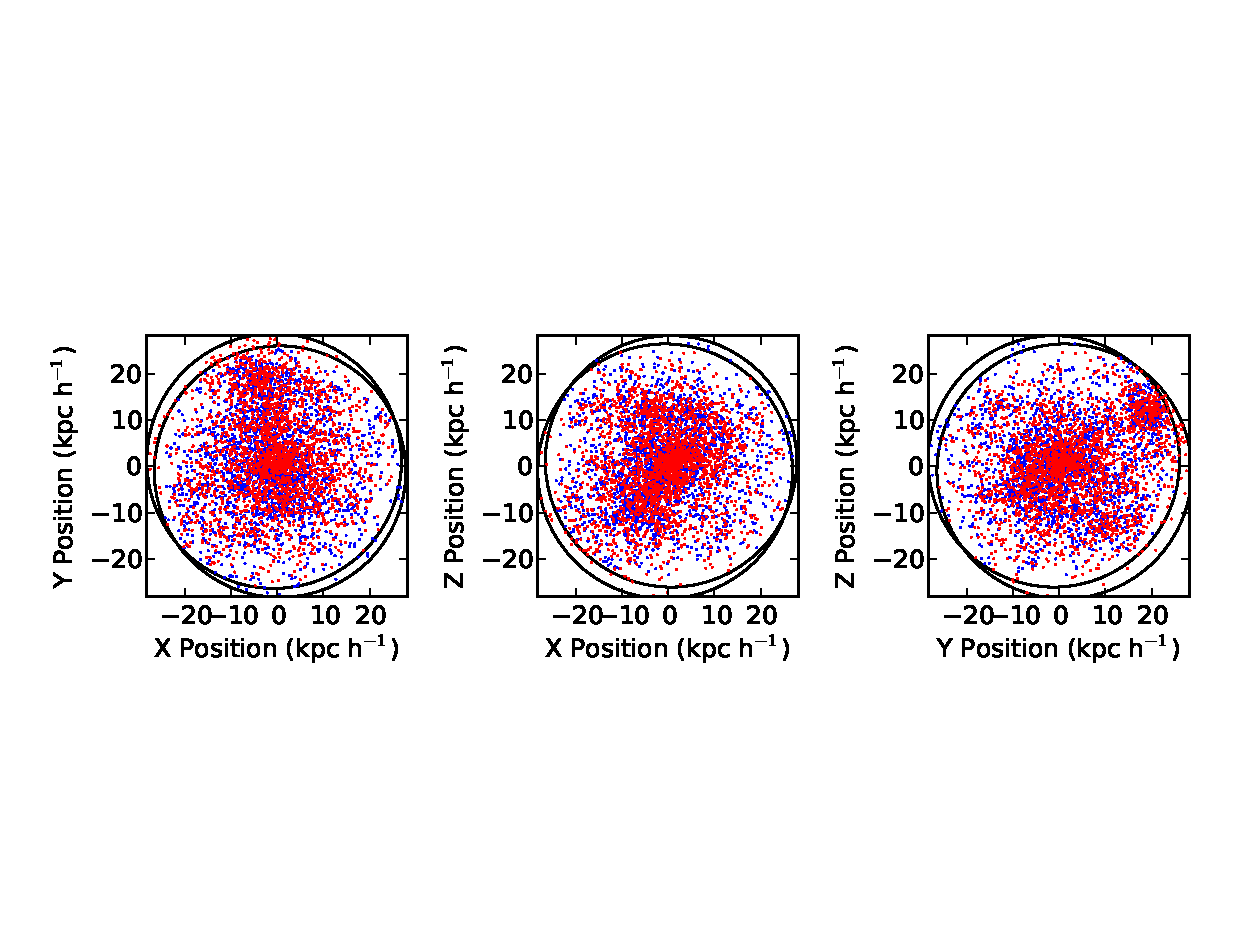
\includegraphics[width=\linewidth]{analysis/match_particles.eps}
	\caption[Example of halo particle matching at $z = 6$.]{\footnotesize Example of halo particle matching at $z = 6$.  Blue dots are \lpt\ halo particles, and red dots are \za\ halo particles.  Black circles are the virial radii of the halos.  Good matches are achieved for halos, with only slight drift between simulations.}
	\label{fig:match_verification}
\end{figure}



%:::::::::::::::::::::::::::::::::::::::::::::::::::::::::::::::::::::::::::::::
\subsubsection{Morphology}
\label{subsubsec:analysis--halo_comparison--morphology}
%:::::::::::::::::::::::::::::::::::::::::::::::::::::::::::::::::::::::::::::::


The morphology of a dark matter halo can provide insight into its structural evolution and merger history.  Features such as tidal tails, irregular shapes, and offset nuclei hint at recent merger activity, while more symmetrical distributions suggest a quieter recent history.  We compare DM particle distributions of matched halos by observing the projected density map along three axis vectors as a guide to lead the discussion of halo merger histories.  The python code for plotting these, as well as the density profiles discussed below, is listed in Appendix~\ref{app:density_comparison}.

By comparing the projected density morphologies of companion \lpt\ and \za\ halos, we get a qualitative impression of the differences in their current evolutionary state.  We found the inner nuclear region to often display the most discernible difference in structure between the two halos.  For halo pairs where this difference is most apparent, such as one halo having a single central core with the other halo having two distinct density peaks, we believe the most likely cause to be an offset in merger epochs between the two simulations.  In this case, the snapshot from one simulation would catch the merger in progress, with multiple unsettled density peaks still visible, while the other simulation snapshot would catch the halo after it has settled into a more virialized state.

As an example of this, we plot comparisons of two $z = 6$ halo pairs in Figures~\ref{fig:density_comparison_000} and~\ref{fig:density_comparison_070}.  The top two rows of panels of each show XY, XZ, and YZ projections of the dark matter density for the \lpt\ and \za\ halo on the first and second row, respectively.  The density map is shown with a logarithmic color scale, and equal density contours are marked with white curves.  Figure~\ref{fig:density_comparison_000} shows a pair of large halos that display similar central structure.  These halos are unlikely to have largely differed in their evolution shortly prior to the snapshot.  Figure~\ref{fig:density_comparison_070}, however, shows a halo pair with differing nuclear structure.  The \za\ halo displays two distinct central density peaks, while the \lpt\ halo shows only a single more relaxed core.

\begin{figure}[tp]
	\centering
	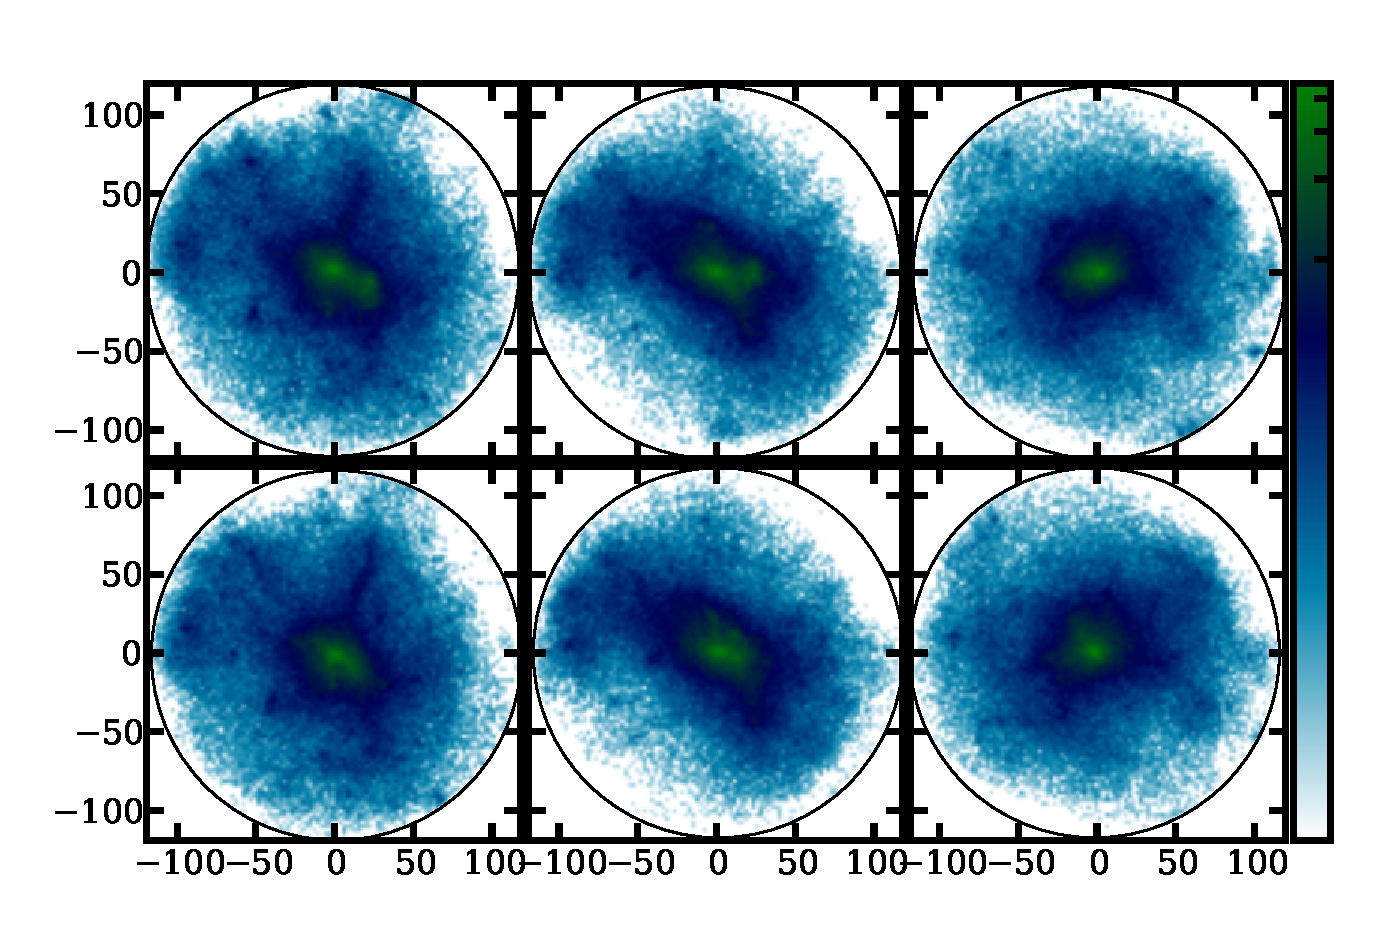
\includegraphics[width=0.75\linewidth]{analysis/halo-pair_000_snap061.eps}
	\caption[Comparison of two large well-fit companion halos $z = 6$.]{\footnotesize Two large matched halos at $z = 6$ with similar nuclear structure.  \emph{Top two rows:}  Projected density maps, with XY, XZ, and YZ views of the central nuclear region of the halos.  Density is represented by a logarithmic color scale, and equal density contours are plotted as white curves.  The first and second rows depict the \lpt\ and \za\ halo, respectively.  \emph{Bottom two rows:}  Radially-binned halo density profiles fit with the NFW density profile model.  The blue stepped profiles are the binned data, red curves are the fit NFW models, black dashed lines are the resolution limit of the simulation, and purple dot-dash lines are the measured scale radius.}
	\label{fig:density_comparison_000}
\end{figure}

\begin{figure}[tp]
	\centering
	\includegraphics[width=0.75\linewidth]{analysis/halo-pair_070_snap061.eps}
	\caption[Comparison of two large companion halos $z = 6$ with differing nuclear structure.]{\footnotesize Like Figure~\ref{fig:density_comparison_000}, but for two large matched halos at $z = 6$ with differing nuclear structure.}
	\label{fig:density_comparison_070}
\end{figure}



%:::::::::::::::::::::::::::::::::::::::::::::::::::::::::::::::::::::::::::::::
\subsubsection{Density Profiles}
\label{subsubsec:analysis--halo_comparison--density_profiles}
%:::::::::::::::::::::::::::::::::::::::::::::::::::::::::::::::::::::::::::::::


The code listed in Appendix~\ref{app:density_comparison}, which produces the density projections discussed above, also plots comparisons of the halos' density profiles.  We have addressed the creation of density profiles in Section~\ref{subsec:analysis--profile_fitting}, and here the same method is used for each profile.  In this case, we with to directly compare the profiles of the companion \lpt\ and \za\ halos, so they are plotted together, alongside the 2-D density projections discussed in the previous section.

We again consider the halo pairs compared in Figures~\ref{fig:density_comparison_000} and~\ref{fig:density_comparison_070}, where the bottom two panels of each display the density profiles of the \lpt\ and \za\ halos, respectively.  Halo particles are binned in logarithmically-spaced radial bins from the virial radius inward to the simulation resolution limit.  The profiles are fit with the NFW profile model with free parameters for scale radius and characteristic density.  The resulting fit is overplotted as red curves, and the scale radius is marked with the vertical purple dot-dash lines.

The halos in Figure~\ref{fig:density_comparison_000} display very similar central morphology and are both well-fit by the NFW profile.  The more relaxed and spherically symmetrical halos such as these tend to be easier to fit well than more irregular halos.  The measured scale radii for these halos are also very similar, and combined with the similar virial radii, produce similar concentration values.  The halos in Figure~\ref{fig:density_comparison_070} display a more differing structure.  While the \lpt\ halo is relatively symmetrical, the \za\ halo has two distinct central density peaks.  Here, there is a marked difference in the resulting scale radii, with the \lpt\ halo displaying a larger concentration than its \za\ companion.




%~~~~~~~~~~~~~~~~~~~~~~~~~~~~~~~~~~~~~~~~~~~~~~~~~~~~~~~~~~~~~~~~~~~~~~~~~~~~~~~
\subsection{Difference Distributions}
\label{subsec:analysis--difference_histograms}
%~~~~~~~~~~~~~~~~~~~~~~~~~~~~~~~~~~~~~~~~~~~~~~~~~~~~~~~~~~~~~~~~~~~~~~~~~~~~~~~


We now turn our focus to the ensemble halo population as a whole.  Comparing individual companion halos can realistically only give a qualitative picture of differences arising between \lpt\ and \za\ simulations, as the large number of halos necessitates consideration of only a small percentage of the sample.  We therefore need a consistent way of measuring the behavior of the entire population.  In this section, we discuss how we measure these differences in halo populations using the codes listed in Appendix~\ref{app:diff_hist}.  In particular, the analysis code itself is listed in Appendix~\ref{app:hist}, the script to run the analysis on the combined halo population from all three simulation boxes is listed in Appendix~\ref{app:run_diff_hist}, the script to run the analysis on the simulation boxes independently is listed in Appendix~\ref{app:run_diff_hist_individual_boxes}, and the script to collect the resulting statistics from all the individual snapshots into one database is listed in Appendix~\ref{app:collect_stats}.



%:::::::::::::::::::::::::::::::::::::::::::::::::::::::::::::::::::::::::::::::
\subsubsection{Histograms}
\label{subsubsec:analysis--difference_histograms--binning}
%:::::::::::::::::::::::::::::::::::::::::::::::::::::::::::::::::::::::::::::::


We wish to explore differences in a number of halo properties, so we construct a generic distribution so that any measured halo quantity $q$ can be considered.  The distribution should  highlight the differences between \lpt\ and \za\ halo populations while remaining unbiased to the choice of simulation initialization.  This leaves us with a distribution of the differences between \lpt\ and \za\ quantities, normalized by the average of the two:
\begin{equation} \label{eq:analysis--delta_q}
	\Delta q = \frac{q_{\lpt} - q_{\za}}{q_{\mathrm{avg}}},
\end{equation}
where $q_{\mathrm{avg}} = \frac{1}{2} (q_{\lpt} + q_{\za})$.  Defined in this way, difference distributions of, e.g.,  virial mass $\Delta \Mvir$, concentration $\Delta c$, or the offset distance between the central density peak and the center of mass $\Delta \Xoff$ can all be considered on equal footing.  We create distribution histograms of $\Delta q$ for various halo quantities both for the combined halo catalog from the stacked simulation boxes and for the individual simulation boxes separately.


%:::::::::::::::::::::::::::::::::::::::::::::::::::::::::::::::::::::::::::::::
\subsubsection{Fitting}
\label{subsubsec:analysis--difference_histograms--fitting}
%:::::::::::::::::::::::::::::::::::::::::::::::::::::::::::::::::::::::::::::::


In order to extract a number of statistical quantities and to get a better high-level feel for the leading behavior of the distributions, we wish to fit a statistical model to the data histograms.  While the data would seem to be distributed according to a Gaussian distribution at first glance, we found the deviations from Gaussianity to be more significant than could be ignored.  After significant trial and error, we found the $\Delta q$ distributions to be best described by a generalized normal distribution \citep{doi:10.1080/02664760500079464} with the probability density function
\begin{equation} \label{eq:analysis--generalized_normal}
	f(x) = \frac{ \beta }{2 \alpha \Gamma(1 / \beta)} e^{\left( \left| x - \mu \right| / \alpha \right)^{\beta}},
\end{equation}
where $\mu$ is the mean, $\alpha$ is the scale parameter, $\beta$ is the shape parameter, and $\Gamma$ is the gamma function
\begin{equation} \label{eq:analysis--gamma_function}
	\Gamma(t) = \int_{0}^{\infty} x^{t-1} e^{-x} \dd x.
\end{equation}
The shape parameter $\beta$ is restricted to $\beta \geq 1$.  This allows the distribution to potentially vary from a Laplace distribution ($\beta = 1$) to a uniform distribution ($\beta = \infty$) and includes the normal distribution ($\beta = 2$).  The distribution has variance
\begin{equation} \label{eq:analysis--variance}
	\sigma^{2} = \frac{ \alpha^{2} \Gamma(3/\beta) }{ \Gamma(1/\beta) }
\end{equation}
and excess kurtosis
\begin{equation} \label{eq:analysis--kurtosis}
	\gamma_{2} = \frac{ \Gamma(5/\beta) \Gamma(1/\beta) }{ \Gamma(3/\beta)^{2} } - 3.
\end{equation}
The distribution is symmetric, and thus has no skewness by definition.  As such, the values obtained for the skew of the distribution are measured directly from the data.

We use the CurveFit module from the SciPy library for all of our functional fitting.  CurveFit is a non-linear least squares fitting routine that can fit an arbitrary input function to data with optional uncertainties.  It can return estimates of the free parameters of the model, as well as a covariance matrix used to determine the uncertainties in the fit coefficients.

We found our fitting routine to be fairly sensitive to differences in initial guess of fit coefficients.  CurveFit is not guaranteed to find global minima, and can become stuck in local extrema.  This ends up being most probable when trying to find multiple fit coefficients with large dynamic range.  We found the best way to address this was to scale the data to unity in each dimension whenever possible.  In the case of our difference histograms, the standard deviations of the distributions are typically around order unity, so it was only necessary to normalized the counts.  We also found that we achieved better results when fitting in logarithmic space.

We explored a number of halo parameters, but found the most interesting distributions to be those for virial mass and concentration.  In Figure~\ref{fig:methods--analysis--diff-hist}, we plot histograms of $\Delta \Mvir$ and $\Delta c$ in the left and right columns, respectively, for three representative simulation snapshots at $z = 14.7$, $z = 10.3$, and $z = 6.0$.  Data from the entire sample are plotted as blue histograms, data for the top 25\% of halo pairs, sorted by \lpt\ halo mass, are plotted as grey-filled green histograms, and the generalized normal distribution fits are overplotted as red dashed curves.

\begin{figure*}[tp]
	\centering
	\begin{subfigure}{}
		\includegraphics[width=0.48\linewidth]{analysis/diff-hist_Mvir_snap040_(0.0-1.0).eps}
	\end{subfigure}
	\begin{subfigure}{}
		\includegraphics[width=0.48\linewidth]{analysis/diff-hist_c_snap040_(0.0-1.0).eps}
	\end{subfigure}
	\\
	\begin{subfigure}{}
		\includegraphics[width=0.48\linewidth]{analysis/diff-hist_Mvir_snap050_(0.0-1.0).eps}
	\end{subfigure}
	\begin{subfigure}{}
		\includegraphics[width=0.48\linewidth]{analysis/diff-hist_c_snap050_(0.0-1.0).eps}
	\end{subfigure}
	\\
	\begin{subfigure}{}
		\includegraphics[width=0.48\linewidth]{analysis/diff-hist_Mvir_snap061_(0.0-1.0).eps}
	\end{subfigure}
	\begin{subfigure}{}
		\includegraphics[width=0.48\linewidth]{analysis/diff-hist_c_snap061_(0.0-1.0).eps}
	\end{subfigure}
	\caption[Histograms of $\Delta M_{\mathrm{vir}}$ and $\Delta c$]{\footnotesize Histograms of $\Delta M_{\mathrm{vir}}$ (\textit{left column}) and $\Delta c$ (\textit{right column}) for snapshots at $z = 14.7$, $z = 10.3$, and $z = 6.0$ (\textit{top, middle, and bottom panels, respectively}).  The small gray-filled histograms count only the top 25\% most massive halos.  The main histograms are fit with a generalized normal distribution with parameters for mean, scale, and shape, overplotted as the red dashed line (see Equation~\ref{eq:analysis--generalized_normal}).}
	\label{fig:methods--analysis--diff-hist}
\end{figure*}




%~~~~~~~~~~~~~~~~~~~~~~~~~~~~~~~~~~~~~~~~~~~~~~~~~~~~~~~~~~~~~~~~~~~~~~~~~~~~~~~
\subsection{Redshift Trends}
\label{subsec:analysis--redshift_trends}
%~~~~~~~~~~~~~~~~~~~~~~~~~~~~~~~~~~~~~~~~~~~~~~~~~~~~~~~~~~~~~~~~~~~~~~~~~~~~~~~


Up to this point, we have only considered one snapshot at a time.  While we have observed variations with redshift, this has not been explicitly quantified.  In this section, we consider the statistical quantities derived from the generalized normal distribution fits from the previous section as functions of redshift.  The code used for this analysis is listed in Appendix~\ref{app:redshift_trends}.



%:::::::::::::::::::::::::::::::::::::::::::::::::::::::::::::::::::::::::::::::
\subsubsection{Mean and Standard Deviation}
\label{subsubsec:analysis--redshift_trends--mean_stdev}
%:::::::::::::::::::::::::::::::::::::::::::::::::::::::::::::::::::::::::::::::


Representing the mean and standard deviation of the distributions is relatively straightforward.  For the fit generalized normal distributions, we record values for the mean, uncertainty in the mean, standard deviation, and uncertainty in the standard deviation.  We also record the mean and standard deviation of the underlying distribution as directly measured from the data.

In Figure~\ref{fig:methods--analysis--fit_trends_mean_stdev}, we plot the mean and standard deviation of the distributions for mass and concentration, as well as the rms value derived from the data, all as functions of redshift.  The mean is plotted as blue points with error bars, the standard deviation is plotted as two black dashed lines that represent $\mu \pm \sigma$, and the rms is plotted as a dotted green line.

\begin{figure*}[tp]
	\centering
	\begin{subfigure}{}
		\includegraphics[width=0.75\linewidth]{analysis/mean_stdev_Mvir.eps}
	\end{subfigure}
	\\
	\begin{subfigure}{}
		\includegraphics[width=0.75\linewidth]{analysis/mean_stdev_c_rockstar.eps}
	\end{subfigure}
	\caption[Mean, standard deviation, and rms as functions of redshift for generalized normal fits]{\footnotesize Mean, standard deviation, and rms as functions of redshift for $\Delta M_{\mathrm{vir}}$ (\textit{top}) and $\Delta c$ (\textit{bottom}).  The mean is plotted as blue points, $\mu \pm \sigma$ is plotted as the black dashed curves, and rms values are plotted as a green dotted curve.  The red dashed line is a linear fit to the mean.}
	\label{fig:methods--analysis--fit_trends_mean_stdev}
\end{figure*}

In this case, we wish to be conservative with the error bars on the mean.  Since we have a measurement for the mean both from the fitting distribution and the underlying data, we can incorporate both of these into our result.  The points plotted in Figure~\ref{fig:methods--analysis--fit_trends_mean_stdev} are the mean measured from the fit distribution, and the error bars are the uncertainty in the mean estimated from the least squares routine.  However, if the mean measured directly from the data falls outside the error bars, the error bars are expanded to encompass that measurement.  This is most often not a concern, as the means for most snapshots are very close together.  However, when there is a slight discrepancy between the fit and data values, the error bars will reflect this.



%:::::::::::::::::::::::::::::::::::::::::::::::::::::::::::::::::::::::::::::::
\subsubsection{Skew}
\label{subsubsec:analysis--redshift_trends--skew}
%:::::::::::::::::::::::::::::::::::::::::::::::::::::::::::::::::::::::::::::::


The generalized normal distributions we use to fit our $\Delta q$ histograms are symmetrical by definition and therefore have no inherent skew.  This was a simplifying assumption necessary to use a well-defined distribution as well as reduce the number of free parameters during fitting.  We do note, however, that the skew of our underlying data is often large enough to not be ignored.

Therefore, we need an alternate way to measure skew and its uncertainty.  We use the skew routine from the SciPy statistics library, which defines skew as
\begin{equation} \label{eq:analysis--skew_def}
	\gamma_{1} = \frac{ \mu_{3} }{ \mu_{2}^{3/2} },
\end{equation}
where $\mu_{m}$ are central moments given by
\begin{align} \label{eq:analysis--central_moments}
	\mu_{m} = E[(X - \mu)^{m}] &= \sum_{k} (x_{k} - \mu)^{m} p(x_{k}) \\
	                           &= \sum_{k=0}^{m} (-1)^{m - k} \binom{m}{k} \mu^{m - k} \mu_{k}',
\end{align}
with non-central moments $\mu_{m}'$ given by
\begin{equation} \label{eq:analysis--non-central_moments}
	\mu_{m}' = E[X^{m}] = \sum_{k} x_{k}^{m} p(x_{k}),
\end{equation}
where $p(x_{k})$ is the probability density function.  The skew is then measured from the entire halo sample for the three combined simulation boxes.  Uncertainty in skew is evaluated by taking the skew of the three boxes as independent measurements.  The results for skew as a function of redshift are plotted as blue curves for the $\Delta \Mvir$ and $\Delta c$ distributions in Figure~\ref{fig:methods--analysis--fit_trends_skew_kurtosis}.

\begin{figure*}[tp]
	\centering
	\begin{subfigure}{}
		\includegraphics[width=0.75\linewidth]{analysis/skew_kurtosis_Mvir.eps}
	\end{subfigure}
	\\
	\begin{subfigure}{}
		\includegraphics[width=0.75\linewidth]{analysis/skew_kurtosis_c_rockstar.eps}
	\end{subfigure}
	\caption[Skew and kurtosis as functions of redshift for generalized normal fits]{\footnotesize Skew (blue curve) and excess kurtosis (red curve) from generalized normal distribution fits as functions of redshift for $\Delta M_{\mathrm{vir}}$ (\textit{top}) and $\Delta c$ (\textit{bottom}).  For both plots, the left axis is the scale for kurtosis and the right axis is the scale for skew.}
	\label{fig:methods--analysis--fit_trends_skew_kurtosis}
\end{figure*}



%:::::::::::::::::::::::::::::::::::::::::::::::::::::::::::::::::::::::::::::::
\subsubsection{Kurtosis}
\label{subsubsec:analysis--redshift_trends--kurtosis}
%:::::::::::::::::::::::::::::::::::::::::::::::::::::::::::::::::::::::::::::::


Variable kurtosis is a fundamental part of the generalized normal distribution, so we may therefore derive the kurtosis directly from the fit distribution parameters.  The generalized normal distribution is defined in terms of a shape parameter $\beta$, which does introduce some complexity in the conversion to kurtosis.  The shape parameter is converted to excess kurtosis by way of Equation~\ref{eq:analysis--kurtosis}.  As this definition includes the Gamma function, a number of steps are required to convert the uncertainty in shape parameter to the uncertainty in kurtosis, which we outline below.

The standard deviation of a function $f(x_{1},x_{2},\dots,x_{n})$ is, in general, given by
\begin{equation} \label{eq:analysis--general_stdev}
	s_{f} = \sqrt{\sum_{x} \left( \frac{\partial f}{\partial x} \right)^{2} s_{x}^{2}},
\end{equation}
with summation over all independent variables $x$.  The generalized normal distribution
\begin{equation} \label{eq:analysis--generalized_normal_reprint}
	f(x) = \frac{\beta}{2 \alpha \Gamma(1/\beta)} e^{-(|x - \mu| / \alpha)^{\beta}},
\end{equation}
with mean $\mu$, scale parameter $\alpha$, and shape parameter $\beta$, has excess kurtosis
\begin{equation} \label{eq:analysis--kurtosis_reprint}
	\gamma_{2} = \frac{\Gamma(5/\beta) \Gamma(1/\beta)}{\Gamma(3/\beta)^{2}} - 3.
\end{equation}
The gamma function
\begin{equation} \label{eq:analysis--gamma_function_reprint}
	\Gamma(x) = \int_{0}^{\infty} t^{x-1} e^{-t} \dd t
\end{equation}
has the first derivative
\begin{equation} \label{eq:analysis--gamma_prime}
	\Gamma'(x) = \Gamma(x) \psi_{0}(x),
\end{equation}
where the digamma function $\digamma$ is the derivative of the logarithm of the gamma function and is given by
\begin{equation} \label{eq:analysis--digamma}
	\digamma(x) = \int_{0}^{\infty} \left( \frac{e^{-t}}{t} - \frac{e^{-xt}}{1 - e^{-t}} \right) \dd t
\end{equation}
if the real part of $x$ is positive.

We now apply \eqref{eq:analysis--general_stdev} to \eqref{eq:analysis--kurtosis_reprint} to find the standard deviation of the excess kurtosis:
\begin{align} \label{eq:analysis--kurt_err_partial1}
	s_{\gamma_{2}} &= \sqrt{ \left( \frac{\diff \gamma_{2}}{\diff \beta} \right)^{2} s_{\beta}^{2} } \\
		&= s_{\beta} \frac{\diff \gamma_{2}}{\diff \beta} \\
		&= s_{\beta} \frac{\diff}{\diff \beta} \left[ \frac{\Gamma(5/\beta) \Gamma(1/\beta)}{\Gamma(3/\beta)^{2}} - 3 \right].
\end{align}
Making the substitution $x = 1 / \beta$ and $\diff x = - 1 / \beta^{2} \dd \beta$, taking the derivative, and doing a bit of algebra, we have:
\begin{align} \label{eq:analysis--kurt_err_partial2}
	s_{\gamma_{2}} &= s_{\beta} \frac{\diff \gamma_{2}}{\diff x} \frac{\diff x}{\diff \beta} \\
		&= s_{\beta} \left( -\frac{1}{\beta^{2}} \right) \frac{\diff}{\diff x} \left[ \frac{\Gamma(5x) \Gamma(x)}{\Gamma(3x)} - 3 \right] \\
		&= -s_{\beta} x^{2} \left\{ \frac{\Gamma(3x)^{2} \frac{\diff}{\diff x} [\Gamma(5x) \Gamma(x)] - \Gamma(5x) \Gamma(x) \frac{\diff}{\diff x} [\Gamma(3x)^{2}]}{\Gamma(3x)^{4}} \right\} \\
		&= -s_{\beta} \frac{x^{2}}{\Gamma(3x)^{4}} \left\{ \Gamma(3x)^{2} [5\Gamma(5x) \digamma(5x) \Gamma(x) + \Gamma(5x) \Gamma(x) \digamma(x)] - \Gamma(5x) \Gamma(x) [6\Gamma(3x)^{2} \digamma(3x)] \right\} \\
		&= s_{\beta} \frac{x^{2}}{\Gamma(3x)^{4}} \left\{ 6\Gamma(5x) \Gamma(3x)^{2} \Gamma(x) \digamma(3x) - \Gamma(5x) \Gamma(3x)^{2} \Gamma(x) [5\digamma(5x) + \digamma(x)] \right\} \\
		&= s_{\beta} \frac{x^{2}}{\Gamma(3x)^{4}} \left\{ \Gamma(5x) \Gamma(3x)^{2} \Gamma(x) [6\digamma(3x) - 5\digamma(5x) - \digamma(x)] \right\} \\
		&= s_{\beta} x^{2} \frac{\Gamma(5x) \Gamma(x)}{\Gamma(3x)^{2}} [6\digamma(3x) - 5\digamma(5x) - \digamma(x)].
\end{align}
Substituting back in for $x$ and recognizing an occurrence of $\gamma_{2}$, we have the result
\begin{equation} \label{eq:analysis--kurt_err}
	s_{\gamma_{2}} = s_{\beta} \frac{1}{\beta^{2}} \left( \gamma_{2} + 3 \right) \left[ 6 \digamma(3/\beta) - 5 \digamma(5/\beta) - \digamma(1/\beta) \right],
\end{equation}
with which we can find the uncertainty in the kurtosis given the value and uncertainty of the shape parameter $\beta$.

With a method of determining the uncertainty in kurtosis established, we may now provide an example of the results (which, again, will be discussed in Chapter~\ref{chap:2lpt}).  In Figure~\ref{fig:methods--analysis--fit_trends_skew_kurtosis}, we plot the kurtosis and associated uncertainties as a function of redshift as red curves for distributions of $\Delta \Mvir$ and $\Delta c$.




%~~~~~~~~~~~~~~~~~~~~~~~~~~~~~~~~~~~~~~~~~~~~~~~~~~~~~~~~~~~~~~~~~~~~~~~~~~~~~~~
\subsection{Mass Trends}
\label{subsec:analysis--mass_trends}
%~~~~~~~~~~~~~~~~~~~~~~~~~~~~~~~~~~~~~~~~~~~~~~~~~~~~~~~~~~~~~~~~~~~~~~~~~~~~~~~


So far, our analysis has mostly focused on the behavior of the entire halo sample as a single unit.  However, there is also a wealth of information available when the statistics for our sample are viewed as functions of halo mass.  In this section, we explore our halo ensemble more deeply by dividing into bins of mass and viewing the behavior of the resulting subsamples.  In this way, we are able to explore differences in low- and high-mass halos, as well as quantify the explicit mass dependencies.  The codes used for this analysis are listed in Appendix~\ref{app:mass_trends}.



%:::::::::::::::::::::::::::::::::::::::::::::::::::::::::::::::::::::::::::::::
\subsubsection{Binning and Fitting}
\label{subsubsec:analysis--mass_trends--binning_plotting}
%:::::::::::::::::::::::::::::::::::::::::::::::::::::::::::::::::::::::::::::::


When representing the mass dependence of our various halo properties, we wished to do so in a way that was both straightforward to quantify and visually descriptive of the overall distribution of the data.  We found the best way to accomplish this was to provide a dual representation, with the data both binned in mass for least-squares fitting and binned two dimensionally in mass and $\Delta q$, with a color scale representing bin density, for a human reader to more easily see the relative population of the parameter space.

First, the data is binned on a 2-D grid.  We found this to be the most natural way to visually represent the distribution of the data, as some features like population sparseness at high redshift, asymmetry, and large differences in number between low- and high-mass halos would be more difficult to convey with only average mass bin means and standard deviations.  The binned data are plotted with a logarithmic color scale and smoothed with a Gaussian kernel.

As a technical aside, we note that plotting bins with zero members with a logarithmic color scale naturally leads to poor results.  We counter this by artificially counting one half halo for bins that are otherwise empty, and rescale the color representation to make anything less than one unit per bin display the minimum color value.

As an alternate representation, and mainly for the benefit of a more quantitative analysis, we bin the data along the average halo mass axis.  For each bin, we measure the mean and standard deviation of the data.  The uncertainty in the mean is then calculated as the standard deviation divided by the square root of the number of particles in the bin.  We find a linear fit to the bin means using our standard least-squares approach, weighted by the mean uncertainties.

Example plots are provided in Figures~\ref{fig:methods--analysis--dM-v-Mavg} and~\ref{fig:methods--analysis--dc-v-Mavg} to demonstrate this approach.  The 2-D binned data is plotted using a logarithmic color scale to represent the number density of halos in a given cell.  The bin means and associated uncertainties are plotted as the black points with error bars.  The standard deviation to either side of the mean is plotted as black dotted lines.  The least-squares fit to the bin means is plotted as a solid magenta line.

\begin{figure*}[tp]
	\centering
	\begin{subfigure}{}
		\includegraphics[width=0.75\linewidth]{analysis/dM-v-Mavg_snap050.eps}
	\end{subfigure}
	\\
	\begin{subfigure}{}
		\includegraphics[width=0.75\linewidth]{analysis/dM-v-Mavg_snap061.eps}
	\end{subfigure}
	\caption[$\Delta M_{\mathrm{vir}}$ as a function of $M_{\mathrm{vir,avg}}$]{\footnotesize $\Delta M_{\mathrm{vir}}$ as a function of $M_{\mathrm{vir,avg}}$.  For the 2-D color histogram, halos are counted in rectangular bins and smoothed with a Gaussian kernel with a logarithmic color scale.  The halos are also divided into logarithmically-spaced bins in average virial mass, and the mean for each bin is plotted as a black point.  The black dotted curves are the standard deviation around the mean.  The magenta line is the linear least-squares best fit to the bin means.  The light grey dashed line at $\Delta q = 0$ is provided to guide the eye.  The two panels correspond to snapshots at $z = 10.3$ and $z = 6.0$.  These plots are provided as examples of the output at this stage of the analysis and are further discussed in Chapter~\ref{chap:2lpt}.}
	\label{fig:methods--analysis--dM-v-Mavg}
\end{figure*}

\begin{figure*}[tp]
	\centering
	\begin{subfigure}{}
		\includegraphics[width=0.75\linewidth]{analysis/dc-v-Mavg_snap050.eps}
	\end{subfigure}
	\\
	\begin{subfigure}{}
		\includegraphics[width=0.75\linewidth]{analysis/dc-v-Mavg_snap061.eps}
	\end{subfigure}
	\caption[$\Delta c$ as a function of $M_{\mathrm{vir,avg}}$]{\footnotesize Like Figure~\ref{fig:methods--analysis--dM-v-Mavg}, but for $\Delta c$ instead of $\Delta \Mvir$ as a function of average halo mass.}
	\label{fig:methods--analysis--dc-v-Mavg}
\end{figure*}



%:::::::::::::::::::::::::::::::::::::::::::::::::::::::::::::::::::::::::::::::
\subsubsection{Trends with Redshift}
\label{subsubsec:analysis--mass_trends--redshift_trends}
%:::::::::::::::::::::::::::::::::::::::::::::::::::::::::::::::::::::::::::::::


To better analyze the time evolution of the mass dependence, we need a more compact representation than simply looking at successive individual redshift snapshots.  The most informative individual parameter from these plots is the slope of the linear fit line for $\Delta q$ as a function of average halo mass.  We therefore plot the slopes and associated uncertainties for each snapshot as a function of redshift, with examples for $\Delta \Mvir$ and $\Delta c$ displayed in Figure~\ref{fig:methods--analysis--slopes_delta-v-Mavg}.  The data are then fit with our linear least-squares routine, and the fit is overplotted as a red dashed line.

\begin{figure*}[tp]
	\centering
	\begin{subfigure}{}
		\includegraphics[width=0.75\linewidth]{analysis/slopes_dM-v-Mavg.eps}
	\end{subfigure}
	\\
	\begin{subfigure}{}
		\includegraphics[width=0.75\linewidth]{analysis/slopes_dc-v-Mavg.eps}
	\end{subfigure}
	\caption[Slopes of the $\Delta q$ vs.\ $M_{\mathrm{vir,avg}}$ fit functions.]{\footnotesize Slopes of the $\Delta q$ vs.\ $M_{\mathrm{vir,avg}}$ fit functions.  The top and bottom panels correspond to the $\Delta M_{\mathrm{vir}}$ and $\Delta c$ plots of Figures~\ref{fig:methods--analysis--dM-v-Mavg} and~\ref{fig:methods--analysis--dc-v-Mavg}.  Linear least-squares fits to the data are overplotted as red dashed lines.  These plots are provided as examples of the output at this stage of the analysis and are further discussed in Chapter~\ref{chap:2lpt}.}
	\label{fig:methods--analysis--slopes_delta-v-Mavg}
\end{figure*}




%~~~~~~~~~~~~~~~~~~~~~~~~~~~~~~~~~~~~~~~~~~~~~~~~~~~~~~~~~~~~~~~~~~~~~~~~~~~~~~~
\subsection{Alternate Difference Distributions}
\label{subsec:analysis--alt_diff_dist}
%~~~~~~~~~~~~~~~~~~~~~~~~~~~~~~~~~~~~~~~~~~~~~~~~~~~~~~~~~~~~~~~~~~~~~~~~~~~~~~~


The distributions of $\Delta q$ that have been discussed up to this point are an excellent measure of the overall behavior of the halo population differences between \lpt\ and \za\ simulations.  However, as these distributions rely on the average quantity $q_{\mathrm{avg}} = (q_{\lpt} + q_{\za}) / 2$ for normalization, quantities like the fraction of halo pairs differing by a given amount between simulations are more difficult to extract.  We therefore redefine our distribution quantity to instead use a normalization factor of $q_{\za}$:
\begin{equation} \label{eq:analysis--delta_prime_q}
	\delta q = \frac{q_{\lpt} - q_{\za}}{q_{\za}},
\end{equation}
which allows for a more direct comparison between halo pairs.  Statistics for these distributions are saved alongside the output for $\Delta q$ distributions with the codes in Appendix~\ref{app:diff_hist}.



%:::::::::::::::::::::::::::::::::::::::::::::::::::::::::::::::::::::::::::::::
\subsubsection{Equivalent Displacement}
\label{subsubsec:analysis--alt_diff_dist--equiv_displacment}
%:::::::::::::::::::::::::::::::::::::::::::::::::::::::::::::::::::::::::::::::


The question may be asked why these distributions have not been used all along, as they more readily offer more quantitative values for our halo populations.  Our previous distributions of $\Delta q$ are symmetrical between \lpt\ and \za\ quantities, which allows us to be completely unbiased as to which simulation initialization is correct.  The distributions of $\delta q$ lose this symmetry, and are only defined for $\delta q \geq -1$ for positive quantities like mass and concentration.

For this analysis, we therefore need a way to consider halo pairs that differ by a certain amount in either direction (e.g. pairs that differ in quantity $q$ by 10\%, whether $q$ is larger in \lpt\ or \za).  Rearranging Equation~\ref{eq:analysis--delta_prime_q} yields
\begin{equation}
	q_{\lpt} = (\delta q + 1) q_{\za},
\end{equation}
and making the substitution $x = \delta q + 1$ gives us
\begin{equation}
	q_{\lpt} = x q_{\za}.
\end{equation}
For a given $x$, we want to find $x_{\mathrm{eq}}$ such that $x_{\mathrm{eq}} = 1 / x$.  Substituting now for $x$ and $x_{\mathrm{eq}}$ and rearranging gives us
\begin{equation} \label{eq:analysis--equivalent_q_prime}
	\delta q_{\mathrm{eq}} = \frac{1}{\delta q + 1} - 1,
\end{equation}
the value for which a halo pair with a larger $q$ in \za\ would differ by the same factor as a halo pair with a larger $q$ in \lpt.



%:::::::::::::::::::::::::::::::::::::::::::::::::::::::::::::::::::::::::::::::
\subsubsection{Redshift Trends}
\label{subsubsec:analysis--alt_diff_dist--trends}
%:::::::::::::::::::::::::::::::::::::::::::::::::::::::::::::::::::::::::::::::


In Figures~\ref{fig:methods--analysis--frac_err_trends_dq} and~\ref{fig:methods--analysis--frac_err_trends_f}, as an example of the output at this step, we plot statistics for our $\delta q$ distributions as functions of redshift.  In Figure~\ref{fig:methods--analysis--frac_err_trends_dq}, we plot the $\delta q$ of the peak of the distribution, as well as the $\delta q$ values where 50\%, 10\%, and 1\% of halo pairs fall at or above $\delta q$.  In Figure~\ref{fig:methods--analysis--frac_err_trends_f}, we plot the fraction of halo pairs $f_{h}$ that fall outside various $\delta q$ values.  The solid curves represent the fraction of halo pairs that have a \lpt\ mass or concentration at least 1.1, 1.5, 2.0, or 5.0 times that of the corresponding \za\ halo.  Dashed curves represent the same values, regardless of whether the \lpt\ or \za\ mass or concentration is higher.  This is the same as counting halos that fall above a given $\delta q$ as well as below the corresponding $\delta q_{\mathrm{eq}}$.  The code for creating these plots is listed in Appendix~\ref{app:alt_redshift_trends}.

\begin{figure*}[tp]
	\centering
	\begin{subfigure}{}
		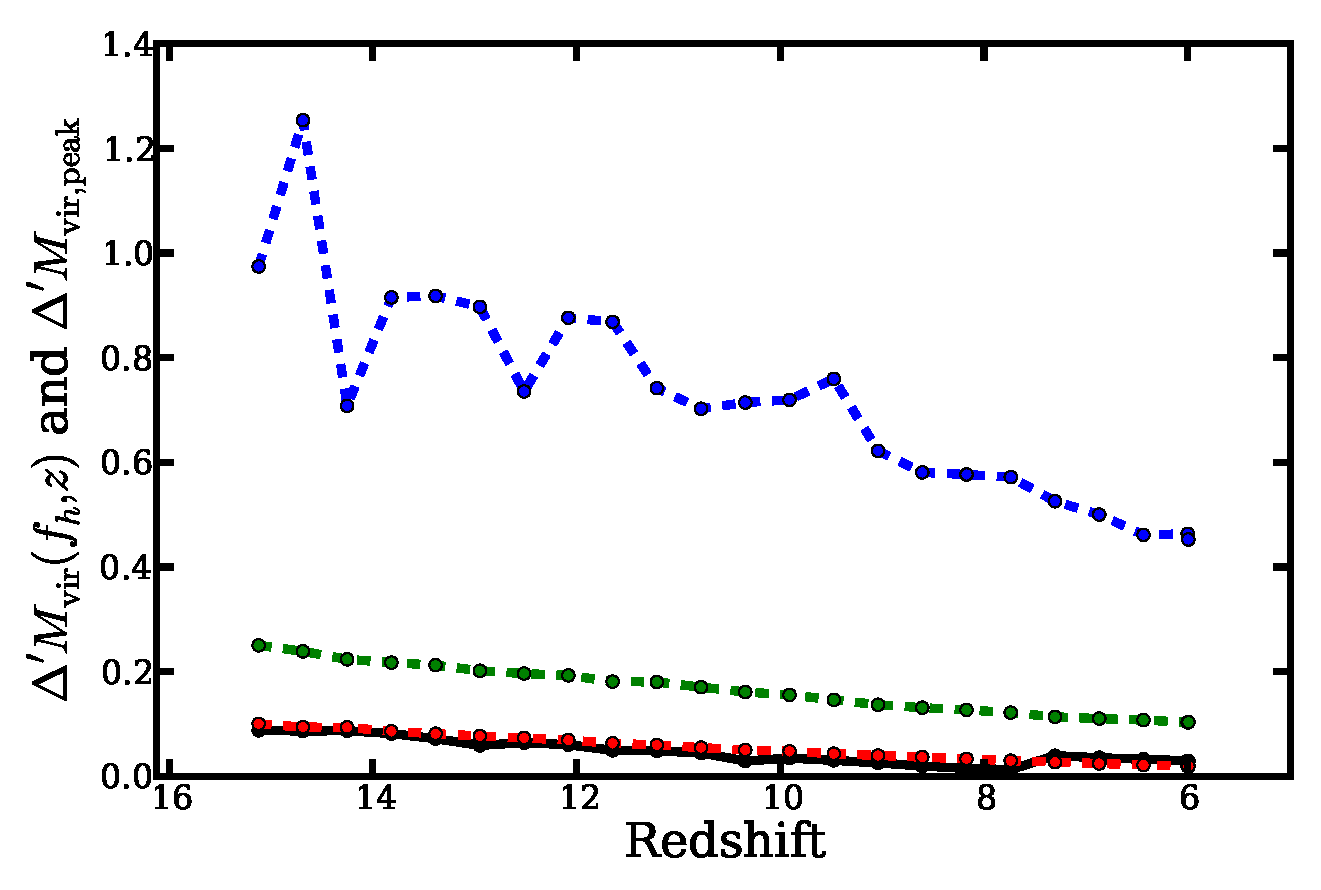
\includegraphics[width=0.75\linewidth]{analysis/percdiff_Mvir_xvals.eps}
	\end{subfigure}
	\\
	\begin{subfigure}{}
		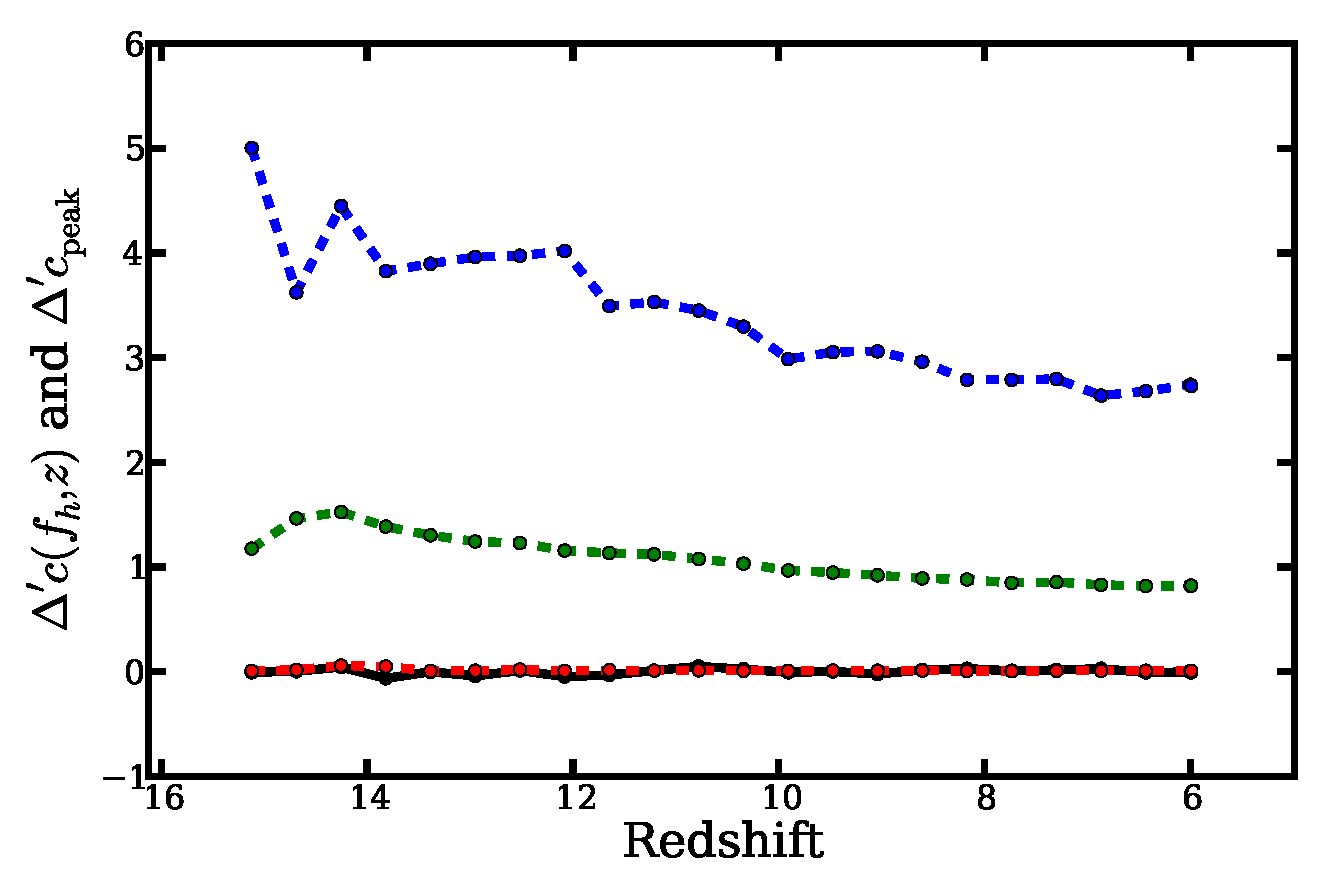
\includegraphics[width=0.75\linewidth]{analysis/percdiff_c_rockstar_xvals.eps}
	\end{subfigure}
	\caption[Statistics for distributions of $\delta q$ as functions of redshift]{\footnotesize Statistics for distributions of $\delta M_{\mathrm{vir}}$ (\textit{top}) and $\delta c$ (\textit{bottom}) as functions of redshift.  The $\delta q$ of the peak of the distribution (black curve), and the $\delta q$ where 50\% (red dashed curve), 10\% (green dashed curve), and 1\% (blue dashed curve) of the halos fall at or above $\delta q$.  These plots are provided as examples of the output at this stage of the analysis and are further discussed in Chapter~\ref{chap:2lpt}.}
	\label{fig:methods--analysis--frac_err_trends_dq}
\end{figure*}

\begin{figure*}[tp]
	\centering
	\begin{subfigure}{}
		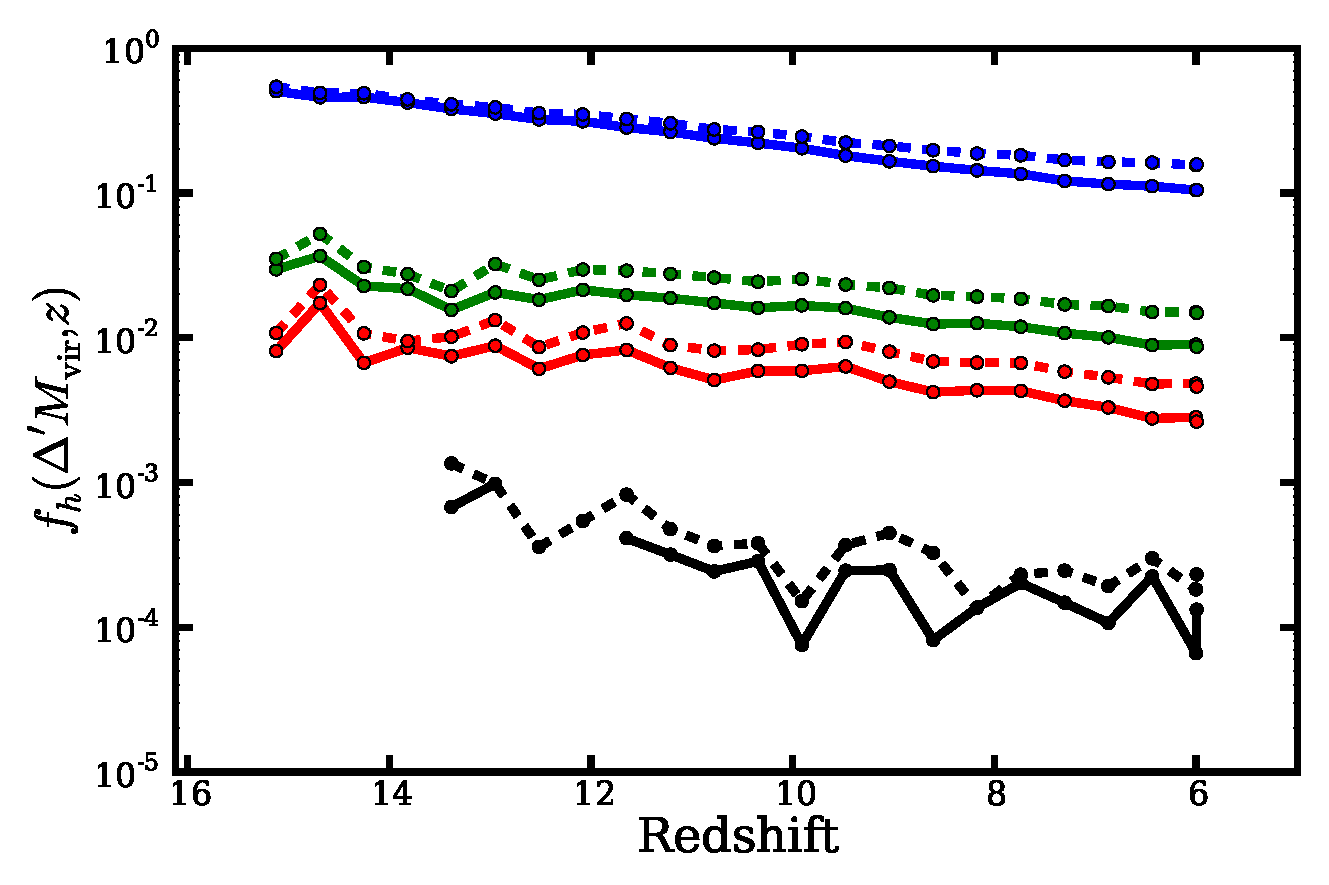
\includegraphics[width=0.75\linewidth]{analysis/percdiff_Mvir_sumfrac.eps}
	\end{subfigure}
	\\
	\begin{subfigure}{}
		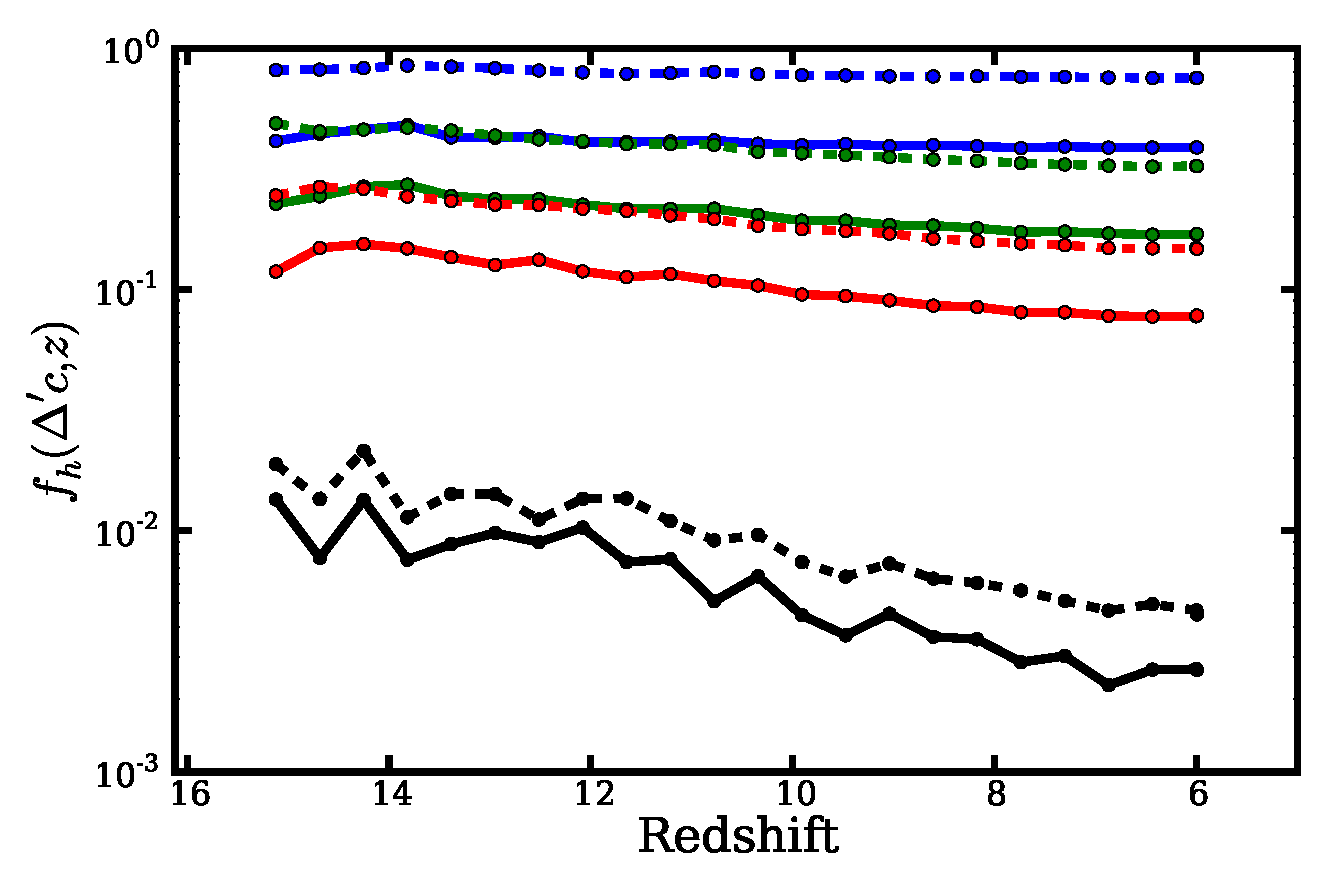
\includegraphics[width=0.75\linewidth]{analysis/percdiff_c_rockstar_sumfrac.eps}
	\end{subfigure}
	\caption[Statistics for distributions of $\delta q$ as functions of redshift]{\footnotesize Statistics for distributions of $\delta M_{\mathrm{vir}}$ (\textit{top}) and $\delta c$ (\textit{bottom}) as functions of redshift.  The fraction of halos with $\delta q$ greater than 0.10 (solid blue curve), 0.50 (solid green curve), 1.00 (solid red curve), and 4.00 (solid black curve).  The dashed curves additionally count halo pairs with $\delta q$ lower than the corresponding equivalent displacements of -0.09, -0.33, -0.50, and -0.80, respectively (see Equation~\ref{eq:analysis--equivalent_q_prime}).  These plots are provided as examples of the output at this stage of the analysis and are further discussed in Chapter~\ref{chap:2lpt}.}
	\label{fig:methods--analysis--frac_err_trends_f}
\end{figure*}






%%%%%%%%%%%%%%%%%%%%%%%%%%%%%%%%%%%%%%%%%%%%%%%%%%%%%%%%%%%%%%%%%%%%%%%%%%%%%%%%
%
% Automation
%
%%%%%%%%%%%%%%%%%%%%%%%%%%%%%%%%%%%%%%%%%%%%%%%%%%%%%%%%%%%%%%%%%%%%%%%%%%%%%%%%

\section{Automation}
\label{sec:automation}

%%%%%%%%%%%%%%%%%%%%%%%%%%%%%%%%%%%%%%%%%%%%%%%%%%%%%%%%%%%%%%%%%%%%%%%%%%%%%%%%


Text goes here.







\chapter{Exploring Dark Matter Halo Populations in \lpt\ and \za\ Simulations}
\label{chap:2lpt}


%%%%%%%%%%%%%%%%%%%%%%%%%%%%%%%%%%%%%%%%%%%%%%%%%%%%%%%%%%%%%%%%%%%%%%%%%%%%%%%%
%
% Exploring Dark Matter Halo Populations in 2LPT and ZA Simulations
%
%%%%%%%%%%%%%%%%%%%%%%%%%%%%%%%%%%%%%%%%%%%%%%%%%%%%%%%%%%%%%%%%%%%%%%%%%%%%%%%%
%
% Chapter Introduction
%
%%%%%%%%%%%%%%%%%%%%%%%%%%%%%%%%%%%%%%%%%%%%%%%%%%%%%%%%%%%%%%%%%%%%%%%%%%%%%%%%


We study the structure and evolution of dark matter halos from $z = 300$ to $z = 6$ for two cosmological N-body simulation initialization techniques.  While the second order Lagrangian perturbation theory (\lpt) and the Zel'dovich approximation (\za) both produce accurate present day halo mass functions, earlier collapse of dense regions in \lpt\ can result in larger mass halos at high redshift.  We explore the differences in dark matter halo mass and concentration due to initialization method through three \lpt\ and three \za\ initialized cosmological simulations.  We find that \lpt\ induces more rapid halo growth, resulting in more massive halos compared to \za.  This effect is most pronounced for high mass halos and at high redshift, with a fit to the mean normalized difference between \lpt\ and \za\ halos as a function of redshift of $\mu_{\Delta M_{\mathrm{vir}}} = (7.88 \pm 0.17) \times 10^{3} z - (3.07 \pm 0.14) \times 10^{-2}$.  Halo concentration is, on average, largely similar between \lpt\ and \za, but retains differences when viewed as a function of halo mass.  For both mass and concentration, the difference between typical individual halos can be very large, even for symmetrically distributed quantities, highlighting the shortcomings of \za-initialized simulations for high-$z$ halo population studies.






%%%%%%%%%%%%%%%%%%%%%%%%%%%%%%%%%%%%%%%%%%%%%%%%%%%%%%%%%%%%%%%%%%%%%%%%%%%%%%%%
%
% Introduction
%
%%%%%%%%%%%%%%%%%%%%%%%%%%%%%%%%%%%%%%%%%%%%%%%%%%%%%%%%%%%%%%%%%%%%%%%%%%%%%%%%

\section{Introduction}
\label{sec:introduction}

%%%%%%%%%%%%%%%%%%%%%%%%%%%%%%%%%%%%%%%%%%%%%%%%%%%%%%%%%%%%%%%%%%%%%%%%%%%%%%%%




%~~~~~~~~~~~~~~~~~~~~~~~~~~~~~~~~~~~~~~~~~~~~~~~~~~~~~~~~~~~~~~~~~~~~~~~~~~~~~~~
% Structure formation in the pre-reionization epoch
%~~~~~~~~~~~~~~~~~~~~~~~~~~~~~~~~~~~~~~~~~~~~~~~~~~~~~~~~~~~~~~~~~~~~~~~~~~~~~~~


The pre-reionization epoch is a time of significant evolution of early structure in the universe.  Rare density peaks in the otherwise smooth dark matter (DM) sea lead to the collapse and formation of the first dark matter halos.  For example, at $z = 20$, $10^{7}~\mathrm{M}_{\odot}$ halos are $\sim 4\sigma$ peaks, and $10^{8}~\mathrm{M}_{\odot}$ halos, candidates for hosting the first supermassive black hole seeds, are $\sim 5\sigma$ peaks.

These early-forming dark matter halos provide an incubator for the baryonic processes that transform the surrounding space and allow galaxies to form.  Initial gas accretion can lead to the formation of the first Pop-III stars \citep{1986MNRAS.221...53C, 1997ApJ...474....1T, 2000ApJ...540...39A, 2002Sci...295...93A}, which, upon their death, can collapse into the seeds for supermassive black holes (SMBHs) \citep{2001ApJ...551L..27M, 2003MNRAS.340..647I, 2009ApJ...701L.133A, 2012ApJ...754...34J} or enrich the surrounding medium with metals through supernovae \citep{2002ApJ...567..532H, 2003ApJ...591..288H}.  The radiation from these early quasars \citep{1987ApJ...321L.107S, 1999ApJ...514..648M, 2001AJ....122.2833F}, Pop-III stars \citep{1997ApJ...486..581G, 2003ApJ...584..621V, 2006ApJ...639..621A}, and proto-galaxy stellar populations \citep{2012ApJ...752L...5B, 2012MNRAS.423..862K} all play a key role in contributing to the re-ionizing of the universe by around $z = 6$ \citep{2001PhR...349..125B}.  Additionally, halo mergers can drastically increase the temperature of halo gas through shock heating, increasing X-ray luminosity \citep{2009MNRAS.397..190S}, and contribute to the unbinding of gas to form the warm-hot intergalactic medium \citep{2008SSRv..134..141B, 2010MNRAS.405L..31S, 2012MNRAS.425.2974T}.




%~~~~~~~~~~~~~~~~~~~~~~~~~~~~~~~~~~~~~~~~~~~~~~~~~~~~~~~~~~~~~~~~~~~~~~~~~~~~~~~
% Current knowledge of high z mass, concentration, and density
%~~~~~~~~~~~~~~~~~~~~~~~~~~~~~~~~~~~~~~~~~~~~~~~~~~~~~~~~~~~~~~~~~~~~~~~~~~~~~~~


While a number of parameters are required to fully characterize a DM halo, a first-order description can be obtained from its mass and density profile.  There are a number of ways to define a halo's mass, the subtleties of which becomes significant for mass-sensitive studies, such as the halo mass function \citep{1974ApJ...187..425P, 2007MNRAS.374....2R, 2006ApJ...642L..85H, 2007ApJ...671.1160L}.  For a review, see, e.g., \citet{2001A&A...367...27W} and references therein.  Additionally, see \citet{2005RvMP...77..207V} and references therein for a more observation-focused discussion.

From a simulation standpoint, the two most common ways to obtain halo mass are to define either spherical overdensity halos or friends-of-friends (FOF) halos.  The spherical overdensity method identifies regions above a certain density threshold, either with respect to the critical density $\rho_{c} = 3 H^{2} / 8 \pi G$ or the background density $\rho_{b} = \Omega_{m} \rho_{c}$, where $\Omega_{m}$ is the matter density of the universe.  The mass is then the mass enclosed in a sphere of some radius with mean density $\Delta \rho_{c}$, where $\Delta$ commonly ranges from $\sim 100$ to $\sim 500$.  Alternatively, the FOF method finds particle neighbors and neighbors of neighbors defined to be within some separation distance \citep{1984MNRAS.206..529E, 1985ApJ...292..371D}.  Halo mass, then, is simply the sum of the masses of the constituent particles.

The density profile of a DM halo is determined by radially binning the constituent particles into spherical shells, and determining the average density per shell, giving a characteristic $\rho(r)$.  The most widely used model for the DM halo density profile is the NFW \citep{1996ApJ...462..563N} profile
\begin{equation} \label{eq:nfw_profile}
	\rho(r) = \frac{ \rho_{0} }{ \frac{ r }{ R_{s}} \left( 1 + \frac{r}{R_{s}} \right)^{2} },
\end{equation}
where $\rho_{0}$ is the characteristic density, and the scale radius $R_{s}$ is the break radius between the inner $\sim r^{-1}$ and outer $\sim r^{-3}$ density profiles.

The halo density profile is quantified by the halo concentration $c \equiv R_{\mathrm{vir}} / R_{s}$.  $R_{\mathrm{vir}}$ is the halo virial radius, which is often defined as the radius at which the average interior density is some factor $\Delta_{c}$ times the critical density of the universe $\rho_{c}$, where $\Delta_{c}$ is typically $\sim 200$.  Generally, at low redshift, low mass halos are more dense than high mass halos \citep{1997ApJ...490..493N}, and concentration decreases with redshift and increases in dense environments \citep{2001MNRAS.321..559B}.  \citet{2007MNRAS.381.1450N} additionally find that concentration decreases with halo mass.  Various additional studies have explored concentration's dependence on characteristics of the power spectrum \citep{2001ApJ...554..114E}, cosmological model \citep{2008MNRAS.391.1940M}, redshift \citep{2008MNRAS.387..536G, 2011MNRAS.411..584M}, and halo merger and mass accretion histories \citep{2002ApJ...568...52W, 2003MNRAS.339...12Z, 2009ApJ...707..354Z}.  For halos at high redshift, \citet{2011ApJ...740..102K} find that concentration reverses and increases with mass for high mass halos, while \citet{2012MNRAS.423.3018P} find that concentration's dependence on mass and redshift is more complicated and is better described through $\sigma(M,z)$, the RMS fluctuation amplitude of the linear density field.




%~~~~~~~~~~~~~~~~~~~~~~~~~~~~~~~~~~~~~~~~~~~~~~~~~~~~~~~~~~~~~~~~~~~~~~~~~~~~~~~
% Simulation initialization
%~~~~~~~~~~~~~~~~~~~~~~~~~~~~~~~~~~~~~~~~~~~~~~~~~~~~~~~~~~~~~~~~~~~~~~~~~~~~~~~


The subtle $\mathcal{O}(10^{-5})$ density perturbations in place at the CMB epoch are vulnerable to numerical noise and intractable to simulate directly.  Instead, a displacement field is applied to the particles to evolve them semi-analytically, nudging them from their initial positions to an approximation of where they should be at a more reasonable starting redshift for the numerical simulation.  Starting at a later redshift saves computation time as well as avoiding interpolation systematics and round-off errors \citep{2007ApJ...671.1160L}.




%~~~~~~~~~~~~~~~~~~~~~~~~~~~~~~~~~~~~~~~~~~~~~~~~~~~~~~~~~~~~~~~~~~~~~~~~~~~~~~~
% 2LPT and ZA
%~~~~~~~~~~~~~~~~~~~~~~~~~~~~~~~~~~~~~~~~~~~~~~~~~~~~~~~~~~~~~~~~~~~~~~~~~~~~~~~


The Zel'dovich approximation \citep{1970A&A.....5...84Z} and 2nd-order Lagrangian Perturbation Theory \citep{1994MNRAS.267..811B, 1994A&A...288..349B, 1995A&A...296..575B, 1998MNRAS.299.1097S} are the two canonical frameworks for the initial particle displacement involved in generating simulation initial conditions.  Zel'dovich approximation (\za, hereafter) initial conditions \citep{1983MNRAS.204..891K, 1985ApJS...57..241E} displace initial particle positions and velocities via a linear field, while 2nd-order Lagrangian Perturbation Theory (\lpt, hereafter) initial conditions \citep{1998MNRAS.299.1097S, 2005ApJ...634..728S, 2010MNRAS.403.1859J} add a second-order correction term to the expansion of the displacement field.

Following \citet{2010MNRAS.403.1859J}, we briefly outline the second-order Lagrangian perturbation theory and compare it to the Zel'dovich approximation.  In \lpt, a displacement field $\boldsymbol{\Psi}(\boldsymbol{q})$ is applied to the initial positions $\boldsymbol{q}$ to yield the Eulerian final comoving positions
\begin{equation} \label{eq:displacement}
	\boldsymbol{x} = \boldsymbol{q} + \boldsymbol{\Psi}.
\end{equation}
The displacement field is given in terms of two potentials $\phi^{(1)}$ and $\phi^{(2)}$ by
\begin{equation} \label{eq:potentials}
	\boldsymbol{x} = \boldsymbol{q} - D_{1} \boldsymbol{\nabla}_{q} \phi^{(1)} + D_{2} \boldsymbol{\nabla}_{q} \phi^{(2)},
\end{equation}
with linear growth factor $D_{1}$ and second-order growth factor $D_{2} \approx -3 D_{1}^{2} / 7$.  The subscripts $\boldsymbol{q}$ refer to partial derivatives with respect to the Lagrangian coordinates $\boldsymbol{q}$.  Likewise, the comoving velocities are given, to second order, by
\begin{equation} \label{eq:velocity}
	\boldsymbol{v} =  - D_{1} f_{1} H \boldsymbol{\nabla}_{q} \phi^{(1)} + D_{2} f_{2} H \boldsymbol{\nabla}_{q} \phi^{(2)},
\end{equation}
with Hubble constant $H$ and $f_{i} = \diff\, \mathrm{ln}\, D_{i} / \diff\, \mathrm{ln}\, a$, with expansion factor $a$.  The relations $f_{1} \approx \Omega^{5/9}$ and $f_{2} \approx 2 \Omega^{6/11}$, with matter density $\Omega$, apply for flat models with a non-zero cosmological constant \citep{1995A&A...296..575B}.  The $f_{1}$, $f_{2}$, and $D_{2}$ approximations here are very accurate for most actual $\Lambda$CDM initial conditions, as $\Omega$ is close to unity at high starting redshift \citep{2010MNRAS.403.1859J}.  We may derive $\phi^{(1)}$ and $\phi^{(2)}$ by solving a pair of Poisson equations
\begin{equation} \label{eq:poisson1}
	\nabla_{q}^{(1)}(\boldsymbol{q}) = \delta^{(1)}(\boldsymbol{q}),
\end{equation}
with linear overdensity $\delta^{(1)}(\boldsymbol{q})$, and
\begin{equation} \label{eq:poisson2}
	\nabla_{q}^{(2)}(\boldsymbol{q}) = \delta^{(2)}(\boldsymbol{q}).
\end{equation}
The second order overdensity $\delta^{(2)}(\boldsymbol{q}$) is related to the linear overdensity field by
\begin{equation} \label{eq:second-order_overdensity}
	\delta^{(2)}(\boldsymbol{q}) = \sum_{i > j} \left\{ \phi_{,ii}^{(1)}(\boldsymbol{q}) \phi_{,jj}^{(1)}(\boldsymbol{q}) - \left[ \phi_{,ij}^{(1)}(\boldsymbol{q}) \right]^{2} \right\},
\end{equation}
where $\phi_{,ij} \equiv \partial^{2} \phi / \partial q_{i} \partial q_{j}$.  For initial conditions from the Zel'dovich approximation, or first-order Lagrangian initial conditions, the $\phi^{(2)}$ terms of Equations~\ref{eq:potentials} and \ref{eq:velocity} are ignored.




%~~~~~~~~~~~~~~~~~~~~~~~~~~~~~~~~~~~~~~~~~~~~~~~~~~~~~~~~~~~~~~~~~~~~~~~~~~~~~~~
% Transients
%~~~~~~~~~~~~~~~~~~~~~~~~~~~~~~~~~~~~~~~~~~~~~~~~~~~~~~~~~~~~~~~~~~~~~~~~~~~~~~~


Cosmological simulations that follow the initial collapse of dark matter density peaks into virialized halos often neglect to consider the nuances of initialization method.  Non-linear decaying modes, or transients, will be damped as $1 / a$ in \za.  In \lpt, however, transients are damped more quickly as $1 / a^{2}$.  It should be expected, then, that structure in \lpt\ will be accurate after fewer $e$-folding times than in \za\ \citep{1998MNRAS.299.1097S, 2006MNRAS.373..369C, 2010MNRAS.403.1859J}.  The practical result is that high-$\sigma$ DM density peaks at high redshift are suppressed in \za\ compared with \lpt\ for a given starting redshift \citep{2006MNRAS.373..369C}.




%~~~~~~~~~~~~~~~~~~~~~~~~~~~~~~~~~~~~~~~~~~~~~~~~~~~~~~~~~~~~~~~~~~~~~~~~~~~~~~~
% In this paper...
%~~~~~~~~~~~~~~~~~~~~~~~~~~~~~~~~~~~~~~~~~~~~~~~~~~~~~~~~~~~~~~~~~~~~~~~~~~~~~~~


While differences in ensemble halo properties, such as the halo mass function, between simulation initialization methods are mostly washed away by $z=0$ \citep{1998MNRAS.299.1097S}, trends at earlier redshifts are less studied \citep{2007ApJ...671.1160L}.  In this paper, we explore the effects of \za\ and \lpt\ on the evolution of halo populations at high redshift.  It is thought that \lpt\ allows initial DM overdensities to get a ``head start'' compared with \za, allowing earlier structure formation, more rapid evolution, and larger possible high-mass halos for a given redshift.  We explore this possibility by evolving a suite of simulations from $z = 300$ to $z = 6$ and comparing the resulting differences in halo properties arising from initialization with \za\ and \lpt\ in these these otherwise identical simulations.

We discuss the simulations, halo finding, and analysis methods in Section~\ref{sec:methods}, results in Section~\ref{sec:results}, implications, caveats, and future work in Section~\ref{sec:discussion}, and a summary of our results and conclusions in Section~\ref{sec:conclusion}.






%%%%%%%%%%%%%%%%%%%%%%%%%%%%%%%%%%%%%%%%%%%%%%%%%%%%%%%%%%%%%%%%%%%%%%%%%%%%%%%%
%
% Numerical Methods
%
%%%%%%%%%%%%%%%%%%%%%%%%%%%%%%%%%%%%%%%%%%%%%%%%%%%%%%%%%%%%%%%%%%%%%%%%%%%%%%%%

\section{Numercial Methods}
\label{sec:2lpt--methods}

%%%%%%%%%%%%%%%%%%%%%%%%%%%%%%%%%%%%%%%%%%%%%%%%%%%%%%%%%%%%%%%%%%%%%%%%%%%%%%%%



%~~~~~~~~~~~~~~~~~~~~~~~~~~~~~~~~~~~~~~~~~~~~~~~~~~~~~~~~~~~~~~~~~~~~~~~~~~~~~~~
% Simulations
%~~~~~~~~~~~~~~~~~~~~~~~~~~~~~~~~~~~~~~~~~~~~~~~~~~~~~~~~~~~~~~~~~~~~~~~~~~~~~~~


We use the Nbody tree/SPH code \gadgettwo\ \citep{2001NewA....6...79S, 2005MNRAS.364.1105S} to evolve six dark matter--only cosmological volumes from $z_{start} = 300$ to $z = 6$ in a $\rm \Lambda CDM$ universe.  Each simulation is initialized using WMAP-5 \citep{2009ApJS..180..330K} parameters.  For each of the three simulation pairs, we directly compare \lpt\ and \za\ by identically sampling the CMB transfer function and displacing the initial particle positions to the same starting redshift using \lpt\ and \za.  The three sets of simulations differ only by the initial phase sampling random seed.  Each volume contains $512^{3}$ particles in a 10 $h^{-1}$ Mpc box.  Full simulation details are discussed in \citet{2012ApJ...761L...8H}.

One facet often overlooked when setting up an \nbody\ simulation is an appropriate starting redshift, determined by box size and resolution \citep{2007ApJ...671.1160L}.  Initialization with \lpt\ allows for a later starting redshift compared with an equivalent \za-initialized simulation.  However, many \za\ simulations do not take this into account, starting from too late of an initial redshift \citep{2006MNRAS.373..369C, 2010MNRAS.403.1859J}.  In order to characterize an appropriate starting redshift, the relation between the initial rms particle displacement and mean particle separation must be considered.  The initial rms displacement $\Delta_{\mathrm{rms}}$ is given by
\begin{equation}
	\Delta_{\mathrm{rms}}^{2} = \frac{4 \pi}{3} \int_{k_{f}}^{k_{\mathrm{Ny}}} P(k, z_{\mathrm{start}}) \dd k,
\end{equation}
where $k_{f} = 2 \pi / L_{\mathrm{box}}$ is the fundamental mode, $L_{\mathrm{box}}$ is the simulation box size, $k_{\mathrm{Ny}} = \frac{1}{2} N k_{f}$ is the Nyquist frequency of an $N^{3}$ simulation, and $P(k, z_{\mathrm{start}})$ is the power spectrum at starting redshift $z_{\mathrm{start}}$.  In order to avoid the ``orbit crossings'' that reduce the accuracy of the initial conditions, $\Delta_{\mathrm{rms}}$ must be some factor smaller than the mean particle separation $\Delta_{p} = L_{\mathrm{box}} / N$ \citep{2012ApJ...761L...8H}.  For example, making orbit crossing a $\sim 10 \sigma$ event imposes $\Delta_{\mathrm{rms}} / \Delta_{p} = 0.1$.  However, for small-volume, high-resolution simulations, this quickly leads to impractical starting redshifts.  Continuing our example, satisfying $\Delta_{\mathrm{rms}} / \Delta_{p} \sim 0.1$ for a $10 h^{-1}$ Mpc, $512^{3}$ simulation suggests $z_{\mathrm{start}} \approx 799$.  Starting at such a high redshift places such a simulation well into the regime of introducing errors from numerical noise caused by roundoff errors dominating the smooth potential.  A more relaxed requirement of $\Delta_{\mathrm{rms}} / \Delta_{p} = 0.25$ yields $z_{\mathrm{start}} = 300$, which we adopt for this work.




%~~~~~~~~~~~~~~~~~~~~~~~~~~~~~~~~~~~~~~~~~~~~~~~~~~~~~~~~~~~~~~~~~~~~~~~~~~~~~~~
% Rockstar
%~~~~~~~~~~~~~~~~~~~~~~~~~~~~~~~~~~~~~~~~~~~~~~~~~~~~~~~~~~~~~~~~~~~~~~~~~~~~~~~


For each of our six simulations, we use the 6-D phase space halo finder code \rockstar\ \citep{2013ApJ...762..109B} to identify spherical overdensity halos at each timestep.  \rockstar\ follows an adaptive hierarchical refinement of friends-of-friends halos in 6-D phase space, allowing determination of halo properties such as halo mass, position, virial radius, internal energy, and number of subhalos.  \rockstar\ tracks halos down to a threshold of around 20 particles, but we use a more conservative 100 particle threshold for our analysis.  We use all particles found within the virial radius to define our halos and their properties.




%~~~~~~~~~~~~~~~~~~~~~~~~~~~~~~~~~~~~~~~~~~~~~~~~~~~~~~~~~~~~~~~~~~~~~~~~~~~~~~~
% CrossMatch
%~~~~~~~~~~~~~~~~~~~~~~~~~~~~~~~~~~~~~~~~~~~~~~~~~~~~~~~~~~~~~~~~~~~~~~~~~~~~~~~


We identify matching halos based on the highest fraction of matching particles contained in each at any given timestep.  We remove subhalo matches (i.e. a halo must not be contained within another halo) and halo pairs with fewer than 100 particles in either \lpt\ or \za.  We are left with approximately 60,000 total halo pairs for our three boxes at $z = 6$.  With halo catalogues matched between simulations, we can compare properties of individual corresponding halos.  To mitigate the effects of cosmic variance on our small volumes, we ``stack'' the three simulation boxes for each initialization method, and combine the halos from each into one larger sample in our analysis.




%~~~~~~~~~~~~~~~~~~~~~~~~~~~~~~~~~~~~~~~~~~~~~~~~~~~~~~~~~~~~~~~~~~~~~~~~~~~~~~~
% Density Profiles
%~~~~~~~~~~~~~~~~~~~~~~~~~~~~~~~~~~~~~~~~~~~~~~~~~~~~~~~~~~~~~~~~~~~~~~~~~~~~~~~


\begin{figure}[t]
    \centering
    \includegraphics[width=\linewidth]{halo-pair_070_snap061.eps}
	\caption[Comparison of matched \lpt\ and \za\ halos]{\footnotesize \textit{Top two rows:}  Density projections for two matching halos at $z = 6$.  The first and second row are \lpt\ and \za, respectively.  The halos appear to be either undergoing or have recently undergone a major merger.  The \lpt\ halo appears to be more relaxed and further along in the merger process, while the \za\ halo lags behind, still displaying two distinct cores.  The halos have masses of $5.95 \times 10^{9} \textrm{M}_{\odot}$ for \lpt\ and $5.85 \times 10^{9} \textrm{M}_{\odot}$ for \za.  \textit{Bottom two rows:}  Density profiles for the same two halos as above.  NFW profiles are fit to logarithmic radial bins of particle position and are overplotted as red curves.  The purple dot--dash lines mark the scale radii.  The black dotted lines mark the resolution limit of the simulations.}
    \label{fig:halo-pair}
\end{figure}

Halo concentration is derived from \rockstar's output for $R_{s}$ and $R_{\mathrm{vir}}$.  Here, $R_{\mathrm{vir}}$ is the virial radius as defined by \citet{1998ApJ...495...80B}.  Figure~\ref{fig:halo-pair} makes evident the difficulty in fitting density profiles and obtaining concentration measurements for typical realistic halos.  Large substructure, as displayed by the \za\ halo, can disrupt the radial symmetry of the halo and cause significant deviations in the density profile.  Centering can also be an issue in these cases.  Due to these complications, there are a number of approaches for finding halo concentrations \citep{2012MNRAS.423.3018P}, but for consistency, we use the values derived from \rockstar's fitting for our concentration measurements.




%~~~~~~~~~~~~~~~~~~~~~~~~~~~~~~~~~~~~~~~~~~~~~~~~~~~~~~~~~~~~~~~~~~~~~~~~~~~~~~~
% Histograms and Curve Fitting
%~~~~~~~~~~~~~~~~~~~~~~~~~~~~~~~~~~~~~~~~~~~~~~~~~~~~~~~~~~~~~~~~~~~~~~~~~~~~~~~


At each simulation snapshot, we measure and compare a number of parameters for halos in both \lpt\ and \za\ simulations.  For each quantity $q$, we create histograms of $\Delta q$, the normalized difference in $q$ between halos in the \lpt\ and \za\ simulations, defined as
\begin{equation} \label{eq:delta_q}
	\Delta q = \frac{q_{\lpt} - q_{\za}}{q_{\mathrm{avg}}},
\end{equation}
where $q_{\mathrm{avg}} = \frac{1}{2} (q_{\lpt} + q_{\za})$.  For each of these, we fit the $\Delta q$ histograms with a generalized normal distribution \citep{doi:10.1080/02664760500079464} with the probability density function
\begin{equation} \label{eq:generalized_normal}
	f(x) = \frac{ \beta }{2 \alpha \Gamma(1 / \beta)} e^{\left( \left| x - \mu \right| / \alpha \right)^{\beta}},
\end{equation}
where $\mu$ is the mean, $\alpha$ is the scale parameter, $\beta$ is the shape parameter, and $\Gamma$ is the gamma function
\begin{equation} \label{eq:gamma_function}
	\Gamma(t) = \int_{0}^{\infty} x^{t-1} e^{-x} \dd x.
\end{equation}
The shape parameter $\beta$ is restricted to $\beta \geq 1$.  This allows the distribution to potentially vary from a Laplace distribution ($\beta = 1$) to a uniform distribution ($\beta = \infty$) and includes the normal distribution ($\beta = 2$).  The distribution has variance
\begin{equation} \label{eq:variance}
	\sigma^{2} = \frac{ \alpha^{2} \Gamma(3/\beta) }{ \Gamma(1/\beta) }
\end{equation}
and excess kurtosis
\begin{equation} \label{eq:kurtosis}
	\gamma_{2} = \frac{ \Gamma(5/\beta) \Gamma(1/\beta) }{ \Gamma(3/\beta)^{2} } - 3.
\end{equation}
The distribution is symmetric, and thus has no skewness by definition.  As such, the values for skew presented below are measured directly from the data.

As our fitting distributions are symmetrical and skew must therefore be measured directly from the data, in order to derive uncertainties for skew, we measure the skew of the distributions for each of our three simulation boxes individually as well as for the single stacked data set.  Uncertainty in skew is then simply the standard deviation of the mean of the skew of the three individual boxes.

Determining the uncertainty in the kurtosis is slightly more involved, as kurtosis is determined by a transformation of the generalized normal distribution's shape parameter $\beta$ according to Equation~\ref{eq:kurtosis}.  Following the standard procedure for propagation of uncertainty, we calculate the standard deviation of the kurtosis as
\begin{align} \label{eq:kurt_err_partial}
    s_{\gamma_{2}} &= \sqrt{ \left( \frac{\diff \gamma_{2}}{\diff \beta} \right)^{2} s_{\beta}^{2} } \\
        &= s_{\beta} \frac{\diff}{\diff \beta} \left[ \frac{\Gamma(5/\beta) \Gamma(1/\beta)}{\Gamma(3/\beta)^{2}} - 3 \right].
\end{align}
The derivative of the gamma function is
\begin{equation} \label{eq:gamma_prime}
    \Gamma'(x) = \Gamma(x) \psi_{0}(x),
\end{equation}
where the digamma function $\digamma$ is the derivative of the logarithm of the gamma function and is given by
\begin{equation} \label{eq:digamma}
    \digamma(x) = \int_{0}^{\infty} \left( \frac{e^{-t}}{t} - \frac{e^{-xt}}{1 - e^{-t}} \right) \dd t
\end{equation}
if the real part of $x$ is positive.  Now, taking the derivative of $\gamma_{2}$ and doing a bit of algebra gives us
\begin{equation} \label{eq:kurt_err}
    s_{\gamma_{2}} = s_{\beta} \frac{1}{\beta^{2}} \left( \gamma_{2} + 3 \right) \left[ 6 \digamma(3/\beta) - 5 \digamma(5/\beta) - \digamma(1/\beta) \right],
\end{equation}
with which we can find the uncertainty in the kurtosis given the value and uncertainty of the shape parameter $\beta$ estimated from the least squares fit routine.

In addition to distributions of $\Delta q$, we also consider distributions of
\begin{equation} \label{eq:delta_prime_q}
	\Delta' q = \frac{q_{\lpt} - q_{\za}}{q_{\za}}
\end{equation}
in order to better quantify the fraction of halos differing by a given amount between \lpt\ and \za\ simulations.  This distribution is inherently non-symmetrical, and is only defined for $\Delta' q \geq -1$ for positive quantities like mass and concentration.  In order to consider halo pairs that differ by a certain amount in either direction (e.g. pairs that differ by 10\%, whether larger in \lpt\ or \za), a relation for equivalent displacement is required.  Rearranging Equation~\ref{eq:delta_prime_q} yields
\begin{equation} \label{eq:delta_prime_q_rearranged}
	q_{\lpt} = (\Delta' q + 1) q_{\za},
\end{equation}
and making the substitution $x = \Delta' q + 1$ gives us
\begin{equation} \label{eq:delta_prime_q_x_factor}
	q_{\lpt} = x q_{\za}.
\end{equation}
For a given $x_{1}$, we want an $x_{2}$ such that $x_{2} = 1 / x_{1}$.  Substituting now for $x_{1}$ and $x_{2}$ and rearranging gives us
\begin{equation} \label{eq:equivalent_q_prime}
	\Delta' q_{2} = \frac{1}{\Delta' q_{1} + 1} - 1,
\end{equation}
the value for which a halo pair with a larger $q$ in \za\ would differ by the same factor as a halo pair with a larger $q$ in \lpt\ where $\Delta' q = \Delta' q_{1}$.





%%%%%%%%%%%%%%%%%%%%%%%%%%%%%%%%%%%%%%%%%%%%%%%%%%%%%%%%%%%%%%%%%%%%%%%%%%%%%%%%
%
% Results
%
%%%%%%%%%%%%%%%%%%%%%%%%%%%%%%%%%%%%%%%%%%%%%%%%%%%%%%%%%%%%%%%%%%%%%%%%%%%%%%%%

\section{Results}
\label{sec:2lpt--results}

%%%%%%%%%%%%%%%%%%%%%%%%%%%%%%%%%%%%%%%%%%%%%%%%%%%%%%%%%%%%%%%%%%%%%%%%%%%%%%%%


With our catalog of matched dark matter halos, we directly compare differences in halo properties arising from initialization with \lpt\ vs \za.  We consider halos on a pair--by--pair basis as well as the entire sample as a whole.  Overall, we find \lpt\ halos have undergone more growth by a given redshift than their \za\ counterparts.




%~~~~~~~~~~~~~~~~~~~~~~~~~~~~~~~~~~~~~~~~~~~~~~~~~~~~~~~~~~~~~~~~~~~~~~~~~~~~~~~
\subsection{Individual halo pairs}
%~~~~~~~~~~~~~~~~~~~~~~~~~~~~~~~~~~~~~~~~~~~~~~~~~~~~~~~~~~~~~~~~~~~~~~~~~~~~~~~


We compare large scale morphologies, density profiles, and various other halo properties for halo pairs on an individual halo--by--halo basis for several of the most massive halos.  Morphologies appear similar for most halos, indicating good halo matches between simulations.  However, many pairs display differences in central morphology, such as the number and separation of central density peaks.  We interpret these cases to be examples of differences in merger epochs, in which case one halo may still be undergoing a major merger, while its companion is in a more relaxed post-merger state.  We give an example of one such pair at $z = 6$ in Figure~\ref{fig:halo-pair}.  The top two rows show density projections of the nuclear regions for a large \lpt\ and matching \za\ halo (first and second rows, respectively).  We find  the \za\ halo to contain two distinct density peaks with a separation of $\sim 10$ kpc, while the \lpt\ halo displays only a single core.  On the third and fourth rows, we plot the density profiles of the same two halos (\lpt\ and \za, respectively).  Here, with nearly identical virial radii, we can readily see that the \lpt\ halo is more concentrated than its \za\ counterpart.




%~~~~~~~~~~~~~~~~~~~~~~~~~~~~~~~~~~~~~~~~~~~~~~~~~~~~~~~~~~~~~~~~~~~~~~~~~~~~~~~
\subsection{Differences in ensemble halo properties}
%~~~~~~~~~~~~~~~~~~~~~~~~~~~~~~~~~~~~~~~~~~~~~~~~~~~~~~~~~~~~~~~~~~~~~~~~~~~~~~~


\begin{figure*}[tp]
	\centering
	\begin{subfigure}{}
		\includegraphics[width=0.48\linewidth]{diff-hist_Mvir_snap040_(0.0-1.0).eps}
	\end{subfigure}
	\begin{subfigure}{}
		\includegraphics[width=0.48\linewidth]{diff-hist_c_snap040_(0.0-1.0).eps}
	\end{subfigure}
	\\
	\begin{subfigure}{}
		\includegraphics[width=0.48\linewidth]{diff-hist_Mvir_snap050_(0.0-1.0).eps}
	\end{subfigure}
	\begin{subfigure}{}
		\includegraphics[width=0.48\linewidth]{diff-hist_c_snap050_(0.0-1.0).eps}
	\end{subfigure}
	\\
	\begin{subfigure}{}
		\includegraphics[width=0.48\linewidth]{diff-hist_Mvir_snap061_(0.0-1.0).eps}
	\end{subfigure}
	\begin{subfigure}{}
		\includegraphics[width=0.48\linewidth]{diff-hist_c_snap061_(0.0-1.0).eps}
	\end{subfigure}
	\caption[Histograms of $\Delta M_{\mathrm{vir}}$ and $\Delta c$]{\footnotesize Histograms of $\Delta M_{\mathrm{vir}}$ (\textit{left column}) and $\Delta c$ (\textit{right column}) for snapshots at $z = 14.7$, $z = 10.3$, and $z = 6.0$ (\textit{top, middle, and bottom panels, respectively}).  The small gray-filled histograms count only the top 25\% most massive halos.  The main histograms are fit with a generalized normal distribution, overplotted as red dashed curves, with parameters for mean, scale, and shape (see Equation~\ref{eq:generalized_normal}).  The distributions for $\Delta M_{\mathrm{vir}}$ have positive means and heavier \lpt\ halos, with the most pronounced difference at high redshift.  The distributions shown here have means of $(8.4 \pm 1.8) \times 10^{-2}$, $(4.87 \pm 0.87) \times 10^{-2}$, and $(1.79 \pm 0.31) \times 10^{-2}$, respectively.  The skew of the distribution is also the most positive at high redshift, and shifts toward symmetry by $z = 6$.  The $\Delta c$ distributions remain symmetric about zero and have negligible skew.  The means are consistent with zero, at $(2.6 \pm 2.7) \times 10^{-2}$, $(0.2 \pm 2.6) \times 10^{-2}$, and $(0.3 \pm 1.1) \times 10^{-2}$, respectively.  Both distributions have excess kurtosis consistently larger than that of a standard Gaussian distribution, with a sharp peak and heavy tails.}
	\label{fig:diff-hist}
\end{figure*}

For the halo population as a whole, we examine distributions of virial mass $M_{\mathrm{vir}}$ and concentration $c$.  We plot histograms of $\Delta M_{\mathrm{vir}}$ and $\Delta c$ in the left and right columns, respectively, of Figure~\ref{fig:diff-hist} for redshifts 14.7, 10.3, and 6.0.  For each panel, the blue histogram features the entire halo sample, and the smaller gray-filled green histogram displays only the top 25\% most massive halos, ordered by \lpt\ mass.  Fits to the primary histograms are overplotted as red dashed curves.

Throughout the simulation, we find a tendency for \lpt\ halos to be more massive.  At $z = 15$, the mean of the $\Delta M_{\mathrm{vir}}$ distribution is $(9.3 \pm 1.2) \times 10^{-2}$.  The mean is consistently positive (heavier \lpt\ halos) and is most displaced from zero at high redshift.  The peak of the distribution gradually moves closer to zero as we progress in redshift.  We find the least difference between paired halos for the final snapshot at $z = 6$, with $\mu_{\Delta M_{\mathrm{vir}}} = (1.79 \pm 0.31) \times 10^{-2}$.

The higher-order moments of the $\Delta M_{\mathrm{vir}}$ distribution are of interest as well, as we find significant deviation from a Gaussian distribution.  One may expect this from the non-linear nature of gravitational collapse; the most massive outliers collapse earlier in \lpt, and this head start compounds subsequent evolution.  As we use a symmetrical generalized normal distribution to fit the data, the skew cannot be recovered from the fit itself; we therefore measure deviation from symmetry directly from the data.  By $z = 6$, we observe a rather symmetrical distribution, with both sides of the histogram equally well described by our fit.  However, at higher redshift, we note a marked increase in skewness and deviation from this symmetry.  As redshift increases, we observe an increasing difference between the fit curve and the bins to the left of the histogram peak.

We find the distributions to be much closer to a Laplace distribution than a Gaussian, with shape parameter consistently sitting at or very close to $\beta = 1$.  Compared to a Gaussian distribution, the larger excess kurtosis implies a narrower central peak and heavier outlying tails.  Our fit is constrained such that $\beta \geq 1$, so the kurtosis of the data itself could potentially be higher than the fit implies.

We find no overall preference for more concentrated \lpt\ or \za\ halos.  In contrast to the $\Delta M_{\mathrm{vir}}$ histograms, $\Delta c$ shows very little deviation from symmetry about zero.  Throughout the simulation, we find the distributions to have a mean close to zero and negligible skew.  The widths of the distributions are much larger than those for $\Delta M_{\mathrm{vir}}$, with the standard deviation of the $\Delta c$ distributions consistently about an order of magnitude higher than for $\Delta M_{\mathrm{vir}}$.  As with mass, concentration histograms are sharply peaked with heavy tails, implying a tendency for halo pairs to move towards the extremes of either very similar or very discrepant concentrations.




%:::::::::::::::::::::::::::::::::::::::::::::::::::::::::::::::::::::::::::::::
\subsubsection{Time evolution of mass and concentration differences}
%:::::::::::::::::::::::::::::::::::::::::::::::::::::::::::::::::::::::::::::::


\begin{figure*}[tp]
	\centering
	\begin{subfigure}{}
		\includegraphics[width=0.48\linewidth]{mean_stdev_Mvir.eps}
	\end{subfigure}
	\begin{subfigure}{}
		\includegraphics[width=0.48\linewidth]{skew_kurtosis_Mvir.eps}
	\end{subfigure}
	\\
	\begin{subfigure}{}
		\includegraphics[width=0.48\linewidth]{mean_stdev_c_rockstar.eps}
	\end{subfigure}
	\begin{subfigure}{}
		\includegraphics[width=0.48\linewidth]{skew_kurtosis_c_rockstar.eps}
	\end{subfigure}
	\caption[Statistics as functions of redshift for generalized normal fits]{\footnotesize Mean, standard deviation, and rms (\textit{left column}) and skew and excess kurtosis (\textit{right column}) as functions of redshift for $\Delta M_{\mathrm{vir}}$ (\textit{top row}) and $\Delta c$ (\textit{bottom row}).  In the left column, $\mu$ is plotted as blue points, $\mu \pm \sigma$ is plotted as the black dashed curves, and rms values are plotted as a green dotted curve.  The red dashed line is a linear fit to the mean.  We find a significant trend for $\mu$ for $\Delta M_{\mathrm{vir}}$ to be more positive at higher redshift and gradually shift toward zero as the simulation progresses, with a fit function of $\mu_{\Delta M_{\mathrm{vir}}} = (7.88 \pm 0.17) \times 10^{-3} z - (3.07 \pm 0.14) \times 10^{-2}$.  The mean for $\Delta c$, however, remains at or very near zero for most of the simulation and is fit by $\mu_{\Delta c} = (3.62 \pm 0.95) \times 10^{-3} z - (2.34 \pm 0.84) \times 10^{-2}$.  The $\Delta M_{\mathrm{vir}}$ and $\Delta c$ distributions narrow over time, with a slight decrease in $\sigma$.  In the right column, we plot skew (blue curve) and excess kurtosis (red curve).  Skew is positive for much of the simulation for $\Delta M_{\mathrm{vir}}$, but is much smaller for $\Delta c$.  Kurtosis is large (much more peaked than Gaussian) for both $\Delta M_{\mathrm{vir}}$ and $\Delta c$ throughout much of the simulation, and especially at later redshift.}
	\label{fig:fit_trends}
\end{figure*}

In Figure~\ref{fig:fit_trends}, we more quantitatively assess the evolution of our various trends hinted at in Figure~\ref{fig:diff-hist}.  Here, we plot the mean, root mean square (rms), standard deviation, skew, and kurtosis for $\Delta M_{\mathrm{vir}}$ and $\Delta c$ as functions of redshift.  Uncertainty in the mean is estimated directly from least squares theory.

The mean for $\Delta M_{\mathrm{vir}}$ is positive and highest at high redshift, trending toward zero by the end of the simulation.  Distributions for $\Delta c$ retain means close to and consistent with zero.  Standard deviation decreases slightly for both $\Delta M_{\mathrm{vir}}$ and $\Delta c$.  From $z = 15$ to $z = 6$, standard deviation falls from $(9.0 \pm 1.5) \times 10^{-2}$ to $(6.08 \pm 0.31) \times 10^{-2}$ for $\Delta M_{\mathrm{vir}}$ and from $0.73 \pm 0.11$ to $0.551 \pm 0.026$ for $\Delta c$.

\begin{table}[t]
	\centering
	\caption{Coefficients for linear least squares fits from Figure~\ref{fig:fit_trends}.}
	\begin{tabular}{ c  r  r }
		\toprule
		                           &  \multicolumn{1}{c}{$A$}             &  \multicolumn{1}{c}{$B$} \\
		\cmidrule(l){2-3}
		$\Delta M_{\mathrm{vir}}$  &  $(7.88 \pm 0.17) \times 10^{-3}$  &  $(-3.07 \pm 0.14) \times 10^{-2}$ \\
		$\Delta c$                 &  $(3.62 \pm 0.95) \times 10^{-3}$  &  $(-2.34 \pm 0.84) \times 10^{-2}$ \\
		\bottomrule
	\end{tabular}
	\label{tab:coeffs}
\end{table}

We find least square linear fits for both mean $\Delta M_{\mathrm{vir}}$ vs $z$ and mean $\Delta c$ vs $z$.  Coefficients for slope $A$ and y-intercept $B$ for the fit equation $\mu = A z + B$ are given in Table~\ref{tab:coeffs} for both cases.  We find a significant trend for $\Delta M_{\mathrm{vir}}$, with a slope $\sim 46 \sigma$ from zero.  Conversely, the slope for $\Delta c$ is much smaller and, considering the larger spread of the underlying distributions, can be considered negligible.  For $\Delta M_{\mathrm{vir}}$, the y-intercept coefficient $B$ likely has little meaning in terms of the actual behavior at $z = 0$, as we expect the trend to level out at later redshift.

We do note, however, that the mean can be deceiving as an indicator of total difference between halo populations, especially when it is close to zero as with concentration.  It should be noted that while the mean can indicate a lack of average difference between the whole sample of \lpt\ and \za\ halos, there can still be very large discrepancies between many individually paired halos.  We visualize this by plotting the rms of $\Delta M_{\mathrm{vir}}$ and $\Delta c$, which is plotted as a green dotted curve.  Unlike the mean, standard deviation, and kurtosis, which are measured from fits to the histograms, rms is measured directly from the data and is not dependent on fitting.  The large rms values are indicative of how much overall difference can arise between \lpt\ and \za\ halos, even though the differences may average to zero when considering the entire population.  The rms for both $\Delta M_{\mathrm{vir}}$ and $\Delta c$ starts highest at high redshift---$0.19$ for $\Delta M_{\mathrm{vir}}$ and $0.57$ for $\Delta c$ at $z = 15$---and steadily decreases throughout the simulation, reaching minimums of $0.11$ for $\Delta M_{\mathrm{vir}}$ and $0.45$ for $\Delta c$ by $z = 6$.

Additionally, it is of interest to consider the percentage of halo pairs that are ``wrong'' at some given time, regardless of whether the quantity is higher in \lpt\ or \za.  For example, if we count halos outside a slit of $\epsilon = 10\%$ around $\Delta q = 0$, we find that by $z = 6$, 14.6\% of halo pairs still have substantially mismatched masses, and 74.3\% have mismatched concentrations.  It is evident that a substantial percentage of halo pairs can have markedly different growth histories, even when there is little or no offset in the ensemble halo population average.

Kurtosis is consistently large for both mass and concentration, with a slight increasing trend throughout the simulation for concentration.  It reaches maximum values of $17.5 \pm 2.4$ at redshift 10 for $\Delta M_{\mathrm{vir}}$ and $15.4 \pm 1.0$ at the end of the simulation at redshift 6 for $\Delta c$.  Skew is positive for much of the simulation for mass, but is much smaller for concentration.  We find average skews of $0.39 \pm 0.29$ for $\Delta M_{\mathrm{vir}}$ and $0.045 \pm 0.028$ for $\Delta c$.  These higher moment deviations from Gaussianity again hint at the non-linear dynamics at play in halo formation.

The narrow peak and heavy tails of the distribution may indicate a fair amount of sensitivity to initial differences in halo properties, in that halo pairs that start out within a certain range of the mean are more likely to move closer to the mean, while pairs that are initially discrepant will diverge even further in their characteristics.  This is indicative of the non-linear gravitational influence present during halo evolution, and is further supported by a kurtosis that increases with time.

The skew at high redshift for $\Delta M_{\mathrm{vir}}$ may give another hint at the non-linear halo formation process.  Runaway halo growth causes more massive halos to favor even faster mass accretion and growth.  The positively skewed distributions show a picture of \lpt\ halo growth in which initial differences in mass are amplified most readily in the earliest forming and most massive halos, again indicating the extra kick-start to halo growth provided by \lpt\ initialization.  While the slight decrease in skew with redshift may be counter-intuitive to this notion, it is likely that the large number of newly formed halos begin to mask the signal from the smaller number of large halos displaying this effect.




%:::::::::::::::::::::::::::::::::::::::::::::::::::::::::::::::::::::::::::::::
\subsubsection{Global halo population differences as a function of  halo mass}
%:::::::::::::::::::::::::::::::::::::::::::::::::::::::::::::::::::::::::::::::


\begin{figure*}[tp]
	\centering
	\begin{subfigure}{}
		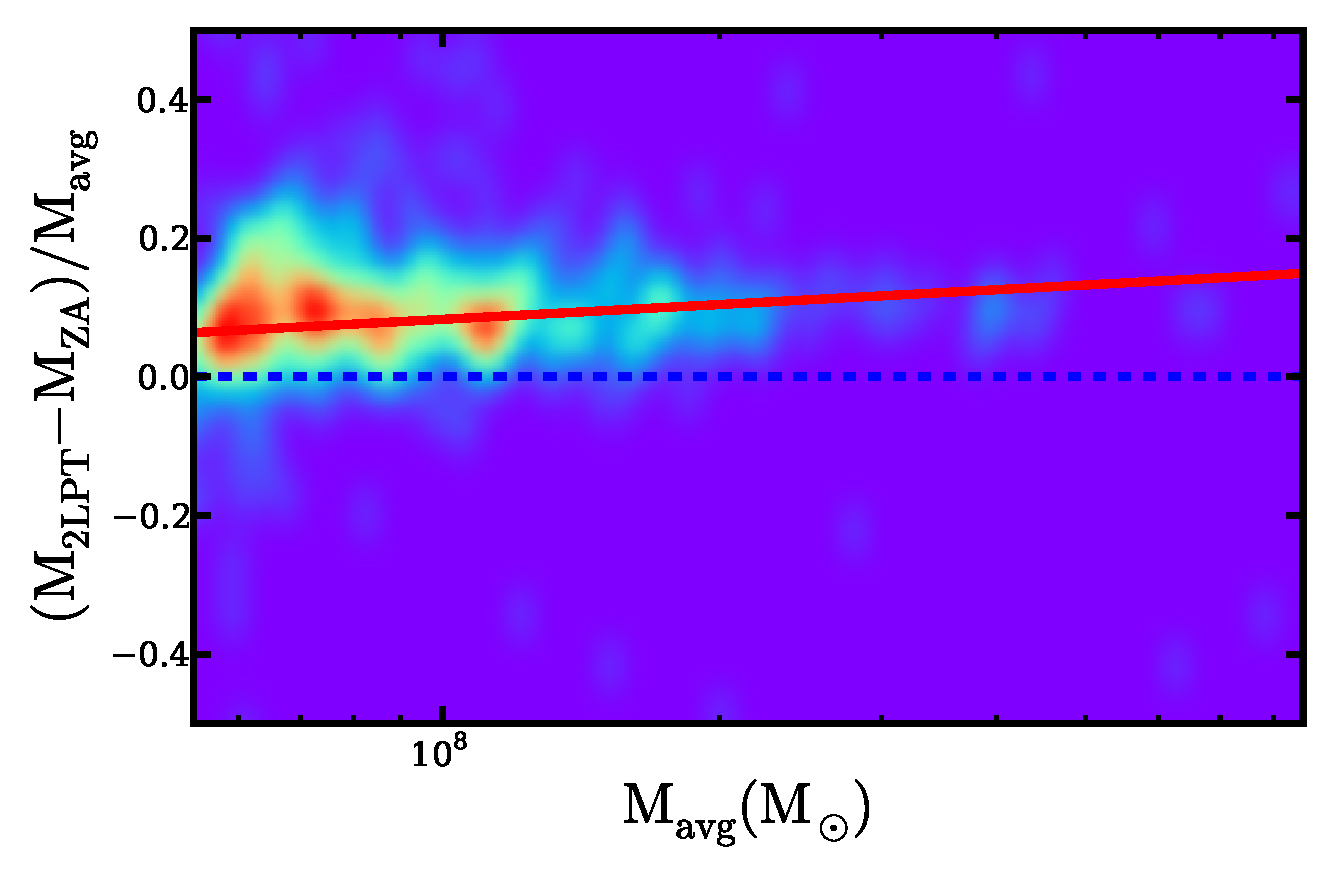
\includegraphics[width=0.48\linewidth]{dM-v-Mavg_snap040.eps}
	\end{subfigure}
	\begin{subfigure}{}
		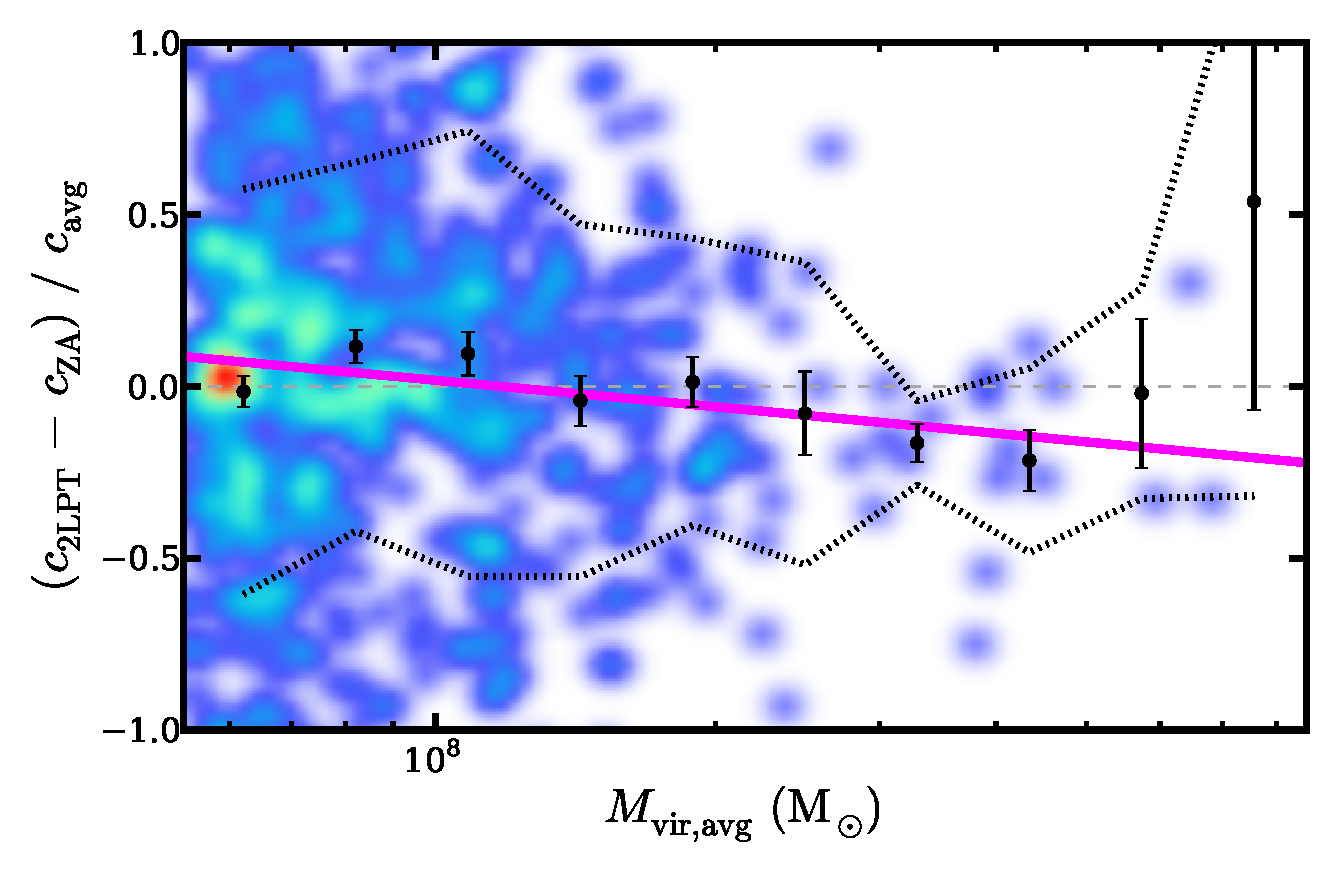
\includegraphics[width=0.48\linewidth]{dc-v-Mavg_snap040.eps}
	\end{subfigure}
	\\
	\begin{subfigure}{}
		\includegraphics[width=0.48\linewidth]{dM-v-Mavg_snap050.eps}
	\end{subfigure}
	\begin{subfigure}{}
		\includegraphics[width=0.48\linewidth]{dc-v-Mavg_snap050.eps}
	\end{subfigure}
	\\
	\begin{subfigure}{}
		\includegraphics[width=0.48\linewidth]{dM-v-Mavg_snap061.eps}
	\end{subfigure}
	\begin{subfigure}{}
		\includegraphics[width=0.48\linewidth]{dc-v-Mavg_snap061.eps}
	\end{subfigure}
	\caption[$\Delta M_{\mathrm{vir}}$ and $\Delta c$ as a function of $M_{\mathrm{vir,avg}}$]{\footnotesize $\Delta M_{\mathrm{vir}}$ (left column) and $\Delta c$ (right column) as functions of $M_{\mathrm{vir,avg}}$.  For the 2-D color histogram, halos are counted in rectangular bins and smoothed with a Gaussian kernel with a logarithmic color scale.  The halos are also divided into logarithmically-spaced bins in average virial mass, and the mean for each bin is plotted as a black point.  The black dotted curves are the standard deviation around the mean.  The magenta line is the linear least-squares best fit to the bin means.  The light grey dashed line at $\Delta q = 0$ is provided to guide the eye.  The three rows again correspond to snapshots at $z = 14.7$, $z = 10.3$, and $z = 6.0$.  We again see the overall offset for positive $\Delta M_{\mathrm{vir}}$ as before, and additionally find a small tendency for more massive halo pairs to be more likely to have even larger $\Delta M_{\mathrm{vir}}$.  Fit equations for the left column panels are $\Delta M_{\mathrm{vir}} = -(0.5 \pm 1.5) \times 10^{-2} \log(M_{\mathrm{vir,avg}}) + (0.15 \pm 0.12)$, $\Delta M_{\mathrm{vir}} = (1.03 \pm 0.46) \times 10^{-2} \log(M_{\mathrm{vir,avg}}) - (2.6 \pm 3.8) \times 10^{-2}$, and $\Delta M_{\mathrm{vir}} = (3.49 \pm 0.99) \times 10^{-3} \log(M_{\mathrm{vir,avg}}) - (6.8 \pm 8.3) \times 10^{-3}$, respectively.  Concentration shows an opposite trend where more massive halos are less concentrated in \lpt\ than in \za.  The right column panels have fit equations $\Delta c = -(0.256 \pm 0.093) \log(M_{\mathrm{vir,avg}}) + (2.07 \pm 0.76)$, $\Delta c = -(7.0 \pm 1.2) \times 10^{-2} \log(M_{\mathrm{vir,avg}}) + (0.595 \pm 0.099)$, and $\Delta c = -(1.10 \pm 0.31) \times 10^{-2} \log(M_{\mathrm{vir,avg}}) + (0.103 \pm 0.026)$, respectively.}
	\label{fig:delta-v-Mavg}
\end{figure*}

\begin{figure*}[tp]
	\centering
	\begin{subfigure}{}
		\includegraphics[width=0.48\linewidth]{slopes_dM-v-Mavg.eps}
	\end{subfigure}
	\begin{subfigure}{}
		\includegraphics[width=0.48\linewidth]{slopes_dc-v-Mavg.eps}
	\end{subfigure}
	\caption[Slopes of the $\Delta q$ vs.\ $M_{\mathrm{vir,avg}}$ fit functions.]{\footnotesize Slopes of the $\Delta q$ vs.\ $M_{\mathrm{vir,avg}}$ fit functions.  The left and right panels correspond to the $\Delta M_{\mathrm{vir}}$ and $\Delta c$ plots in the left and right columns, respectively, of Figure~\ref{fig:delta-v-Mavg}.  Linear least-squares fits to the data are overplotted as red dashed lines.  Overall, we find a trend of positive and increasing slope with redshift for $\Delta M_{\mathrm{vir}}$ and negative and decreasing slope with redshift for $\Delta c$.  We find fit equations of $\mathrm{Slope} = (9.4 \pm 2.4) \times 10^{-4} z - (1.8 \pm 1.8) \times 10^{-3}$ for $\Delta M_{\mathrm{vir}}$ and $\mathrm{Slope} = -(7.3 \pm 1.9) \times 10^{-3} z + (3.7 \pm 1.4) \times 10^{-2}$ for $\Delta c$.  Snapshots at very high redshift, $z \gtrsim 14$ for $\Delta M_{\mathrm{vir}}$ and $z \gtrsim 13$ for $\Delta c$, begin to deviate from these trends.  However, it is uncertain if this deviation is significant due to the low number statistics of our sample at such high $z$.}
	\label{fig:slopes_delta-v-Mavg}
\end{figure*}

We consider $\Delta M_{\mathrm{vir}}$ and $\Delta c$ as a function of average halo mass $M_{\mathrm{vir,avg}} = (M_{\mathrm{vir},\lpt} + M_{\mathrm{vir},\za}) / 2$ for three representative timesteps in Figure~\ref{fig:delta-v-Mavg}.  The data are binned in average virial mass, for which means and standard deviations are provided as the black points and black dotted curves, respectively.  The error bars on the black points represent the uncertainty in the mean and are the standard deviation divided by the number of halos in that bin.  We additionally bin the data in rectangular bins on a 2-D grid with a logarithmic color map to feature the entire distribution of the data.  Linear fits to the bin means are overplotted in magenta.

We find that $\Delta M_{\mathrm{vir}}$ tends to increase with increasing $M_{\mathrm{vir,avg}}$ for most snapshots.  \lpt\ halos are consistently more massive than their \za\ counterparts, and, aside from the highest redshift snapshots, this difference increases with average halo mass.  While less massive halo pairs have a larger spread in the difference in \lpt\ and \za\ mass, more massive halo pairs are consistently heavier in \lpt\ than in \za.  At redshift 14.7, we find a transition between negative and positive slopes, and here the fit is $\Delta M_{\mathrm{vir}} = -(0.5 \pm 1.5) \times 10^{-2} \log(M_{\mathrm{vir,avg}}) + (0.15 \pm 0.12)$.   The slope of the fit lines then become positive and trends back towards zero as we progress in redshift, with a fit of $\Delta M_{\mathrm{vir}} = (3.49 \pm 0.99) \times 10^{-3} \log(M_{\mathrm{vir,avg}}) - (6.8 \pm 8.3) \times 10^{-3}$ by $z = 6$.

We additionally find a trend for more massive halo pairs to be more concentrated in \za.  This trend is somewhat stronger than for $\Delta M_{\mathrm{vir}}$, but again, high $z$ snapshots differ from the trend.  The fit equations for $z = 15$ and $z = 6$ are $\Delta c = -(0.256 \pm 0.093) \log(M_{\mathrm{vir,avg}}) + (2.07 \pm 0.76)$ and $\Delta c = -(1.10 \pm 0.31) \times 10^{-2} \log(M_{\mathrm{vir,avg}}) + (0.103 \pm 0.026)$, respectively.  The negative slope for most of the redshift range might be expected, as halo concentration is expected to decrease with increasing mass for all but the largest halos, where the concentration begins to increase with increasing mass \citep{2011ApJ...740..102K, 2012MNRAS.423.3018P}, and we find that $\Delta M_{\mathrm{vir}}$ increases with average mass for all but the highest redshift snapshots.  The turnover in halo concentrations displayed in \citet{2011ApJ...740..102K} and \citet{2012MNRAS.423.3018P} should be relatively inconsequential for our simulations, as we have a significantly smaller box size, and thus a smaller maximum halo mass.  Additionally, our most massive halos account for a very small percentage of the total halo population, causing the larger number of small halos to be more significant in the resulting fits.  The data have a larger variance than $\Delta M_{\mathrm{vir}}$ by a factor of $\sim 2$.  Again, mass dependence is smallest by $z = 6$.  To reconcile these trends with the symmetrical concentration distributions of Figure~\ref{fig:diff-hist}, we note that the trends in mass may be obscured by integration across the entire mass range and still result in overall $\Delta c$ distributions symmetric about zero.  Additionally, the histograms of Figure~\ref{fig:diff-hist} may be swamped by the large number of low mass halos, which masks the large difference in concentration seen here.

\begin{table}[t]
	\centering
	\caption{Coefficients for linear least squares fits from Figure~\ref{fig:slopes_delta-v-Mavg}.}
	\begin{tabular}{ c  r  r }
		\toprule
		                           &  \multicolumn{1}{c}{$A$}            &  \multicolumn{1}{c}{$B$} \\
		\cmidrule(l){2-3}
		$\Delta M_{\mathrm{vir}}$  &   $(9.4 \pm 2.4) \times 10^{-4}$  &  $(-1.8 \pm 1.8) \times 10^{-3}$ \\
		$\Delta c$                 &  $(-7.3 \pm 1.9) \times 10^{-3}$  &   $(3.7 \pm 1.4) \times 10^{-2}$ \\
		\bottomrule
	\end{tabular}
	\label{tab:coeffs_slopes}
\end{table}

The slopes of the fits to the $\Delta q$ vs.$M_{\mathrm{vir,avg}}$ data are plotted in Figure~\ref{fig:slopes_delta-v-Mavg}.  Linear least-squares fits are overplotted as red dashed lines.  We find a trend for there to be more $\Delta q$ dependence on $M_{\mathrm{vir,avg}}$ with increasing redshift, except for the highest $z$ snapshots, where the trends seem to reverse.  Coefficients $A$ and $B$ for the fit equation $\mathrm{Slope} = A z + B$ are listed in Table~\ref{tab:coeffs_slopes}.  The data are well-fit by the best fit line for most of the redshift range, except for $z \gtrsim 14$ for $\Delta M_{\mathrm{vir}}$ and $z \gtrsim 13$ for $\Delta c$, which begin to deviate from the trend.  While this may simply be due to the fluctuations inherent when dealing with the low number of matched halos available in our sample at these very high redshifts, a shift to positive slope for concentration may be expected.  At these redshifts, only the most massive halos halos fall above our particle threshold, whereas at later redshift, the large number of small halos can overwhelm the statistics.  These massive halos are most affected by high redshift differences due to initialization and may retain larger \lpt\ concentrations due to earlier formation.




%~~~~~~~~~~~~~~~~~~~~~~~~~~~~~~~~~~~~~~~~~~~~~~~~~~~~~~~~~~~~~~~~~~~~~~~~~~~~~~~
\subsection{A census of halo population differences}
%~~~~~~~~~~~~~~~~~~~~~~~~~~~~~~~~~~~~~~~~~~~~~~~~~~~~~~~~~~~~~~~~~~~~~~~~~~~~~~~


\begin{figure*}[tp]
	\centering
	\begin{subfigure}{}
		\includegraphics[width=0.48\linewidth]{percdiff_Mvir_xvals.eps}
	\end{subfigure}
	\begin{subfigure}{}
		\includegraphics[width=0.48\linewidth]{percdiff_Mvir_sumfrac.eps}
	\end{subfigure}
	\\
	\begin{subfigure}{}
		\includegraphics[width=0.48\linewidth]{percdiff_c_rockstar_xvals.eps}
	\end{subfigure}
	\begin{subfigure}{}
		\includegraphics[width=0.48\linewidth]{percdiff_c_rockstar_sumfrac.eps}
	\end{subfigure}
	\caption[Statistics for distributions of $\delta q$ as functions of redshift]{\footnotesize Statistics for distributions of $\delta M_{\mathrm{vir}}$ (\textit{top row}) and $\delta c$ (\textit{bottom row}) as functions of redshift.  \textit{Left column}:  The $\delta q$ of the peak of the distribution (black curve), and the $\delta q$ where 50\% (red dashed curve), 10\% (green dashed curve), and 1\% (blue dashed curve) of the halos fall at or above $\delta q$.  As with distributions of $\Delta M_{\mathrm{vir}}$, $\delta M_{\mathrm{vir}}$ has the largest positive displacement at high redshift and steadily decreases throughout the simulation.  Additionally, $\delta c$ maintains a peak near zero and has a spread much larger than that of $\delta M_{\mathrm{vir}}$.  \textit{Right column}:  The fraction of halos with $\delta q$ greater than 0.10 (solid blue curve), 0.50 (solid green curve), 1.00 (solid red curve), and 4.00 (solid black curve).  The dashed curves additionally count halo pairs with $\delta q$ lower than the corresponding equivalent displacements of -0.09, -0.33, -0.50, and -0.80, respectively (see Equation~\ref{eq:equivalent_q_prime}).  We find that 50\% of \lpt\ halos are at least 10\% more massive than their \za\ companions at $z = 15$, reducing to 10\% by $z = 6$.  Halos in \lpt\ are at least twice as concentrated for 12\% of halos at $z = 15$ and 7.8\% of halos at $z = 6$.}
	\label{fig:frac_err_trends}
\end{figure*}

As our distributions of $\Delta q$ rely on the average quantity $q_{\mathrm{avg}} = (q_{\lpt} + q_{\za}) / 2$ for normalization, it can be difficult to extract certain statistics, such as the fraction of halo pairs differing by a certain amount between \lpt\ and \za\ simulations.  To address this, for this section, we redefine our difference distributions to instead use $q_{\za}$ as the normalization factor (see Equation~\ref{eq:delta_prime_q}).  In Figure~\ref{fig:frac_err_trends}, we plot, as functions of redshift, statistics derived from these alternate fractional difference distributions $\delta M_{\mathrm{vir}}$ and $\delta c$.  In the left column, we plot the $\delta q$ of the peak of the distribution along with the $\delta q$ where various percentages of the halo pairs fall at or above $\delta q$.

As the $\delta q$ value of the peak of the distribution is the location of the mode, it represents the most typical halo pair.  While concentration differences remain close to zero throughout the simulation, the mass difference peak moves from a $\delta M_{\mathrm{vir}}$ of $9 \times 10^{-2}$ at $z = 15$ to $3 \times 10^{-2}$ at $z = 6$.  The 1\% of halo pairs with the largest excess \lpt\ mass have \lpt\ mass at least twice \za\ mass at $z = 15$ and 1.5 times \za\ mass at $z = 6$.  For concentration, the 1\% most \lpt\ concentrated halo pairs differ by at least a factor of 6 at $z = 15$ and 4 at $z = 6$.

In the right column of Figure~\ref{fig:frac_err_trends}, we plot the fraction of halos $f_{h}$ that fall outside various $\delta q$ values.  The solid curves represent halo pairs that have $\delta q$ greater than or equal to the listed values, i.e., the fraction of halo pairs where the \lpt\ halo has a virial mass or concentration that is at least 1.1, 1.5, 2.0, or 5.0 times that of its corresponding \za\ halo.  The dashed curves represent the fraction of halo pairs where one halo has a virial mass or concentration at least 1.1, 1.5, 2.0, or 5.0 times that of its companion, regardless of whether the \lpt\ or \za\ value is higher.

We find that half of halo pairs are at least 10\% more massive in \lpt\ at $z = 15$.  By $z = 6$, this has fallen to 10\%.  Furthermore, 1\% are at least twice as massive in \lpt\ at $z = 15$, and by $z = 6$, this has only reduced to 0.3\%.  Halos in \lpt\ are at least twice as concentrated as their \za\ counterparts for at least 12\% of the halo population at $z = 15$ and at least 8\% by $z = 6$.  Halo pairs that are at least 5 times as concentrated in \lpt\ make up 1.3\% of the sample at $z = 15$ and 0.3\% at $z = 6$.

If we consider only the difference in properties between paired halos, regardless of whether the \lpt\ or \za\ halo has the higher mass or concentration, we include an even larger percentage of the population.   We find 54\% of the halo pairs differ in mass by at least 10\% at $z = 15$, with 16\% differing by $z = 6$.  Halos that are at least twice as massive in either \lpt\ or \za\ account for 1.1\% at $z = 15$ and 0.5\% at $z = 6$.  Halos that are at least twice as concentrated in either \lpt\ or \za\ account for 25\% at $z = 15$ and 15\% at $z = 6$.





\section{Discussion}
\label{sec:discussion}


%\begin{enumerate}
%	\item Implications
%		\begin{enumerate}
%			\item Importance of using \lpt
%			\item Earlier mergers
%			\item More massive halos
%			\item Reionization/PopIII stars
%			\item SMBH formation head start
%			\item Epoch of peak star formation (shifted earlier?)
%			\item Extrapolation (by eye) of slope plot to later $z$
%			\item Abundance matching
%		\end{enumerate}
%	\item Limitations and caveats
%		\begin{enumerate}
%			\item Box size only 10 Mpc - not big enough for large outlier density peaks
%			\item Rockstar nondeterminism
%			\item Substructure
%			\item Halo matching not perfect - mergers at different times \textcolor{red}{Should probably also talk about this in analysis section.}
%			\item Statistics/goodness of fit on concentrations from rockstar
%			\item Fewer halos fit with python density profile code
%			\item Does concentration make sense at high $z$ (not virialized yet)?
%		\end{enumerate}
%	\item Future work
%		\begin{enumerate}
%			\item Bigger box
%			\item More particles
%			\item Start at earlier $z$?
%			\item Run to $z = 0$?
%			\item Other cosmologies?
%			\item Baryons?
%		\end{enumerate}
%\end{enumerate}

As we evolve our DM halo population from our initial redshift to $z = 6$, we find that simulation initialization with \lpt\ can have a significant effect on halo population compared to initialization with \za.  The second order displacement boost of \lpt\ provides a head start on the initial collapse and formation of DM halos.  This head start manifests itself further along in a halo's evolution as more rapid growth and potentially earlier mergers.  \lpt\ halos are, on average, more massive than their \za\ counterparts.  The larger mass for \lpt\ halos is more pronounced for higher mass pairs, while \lpt\ halo concentration is larger on the small mass end.  Both mass and concentration differences trend towards symmetry about zero as halos evolve in time, with the smallest difference observed at the end of the simulations at $z = 6$.  Casual extrapolation of our observed trends with redshift to today would indicate that \lpt\ and \za\ would produce very similar halo populations by $z = 0$.  However, the larger differences at high redshift should not be ignored.

The earlier formation times and larger masses of halos seen in \lpt-initialized simulations could have significant implications with respect to early halo life during the Dark Ages.  Earlier forming, larger halos affect the formation of Pop-III stars, and cause SMBHs to grow more rapidly during their infancy \citep{2012ApJ...761L...8H}.  The epoch of peak star formation may also be shifted earlier.  This could additionally affect the contribution of SMBHs and early star populations to re-ionization.  Larger halos may also influence studies of the high-$z$ halo mass function, abundance matching, gas dynamics, AGN, clustering, and large scale structure formation.

In these discussions, it is important to note that it is wrong to assume that the \za\ halo properties are the ``correct'' halo properties, even in a statistical sense.  While halo mass suggests the most obvious shortcoming of \za\ simulations, even properties such as concentration that show little difference on average between \lpt\ and \za\ can have large discrepancies on an individual halo basis.  Failure to consider uncertainties in halo properties for high $z$ halos in \za\ simulations can lead to catastrophic errors.

We note a few caveats with our simulations and analysis.  We did not exclude substructure when determining the properties of a halo, so care must be taken when comparing to works which remove subhalo particles in determining halo mass and concentration.  Halo matching is not perfect, as it is based on one snapshot at a time, and may miss count halos due to merger activity and differences in merger epochs.  However, we believe this effect to be minor.  While we compared \rockstar's output with our own fitting routines and found them to be in good agreement, \rockstar\ does not provide goodness of fit parameters for its NFW profile fitting and $R_{\mathrm{s}}$ measurements.  It also may be debated whether it makes sense to even consider concentration of halos at high redshift which are not necessarily fully virialized.

We use a simulation box size of only 10 Mpc.  This is too small to effectively capture very large outlier density peaks.  We would, however, expect these large uncaptured peaks to most affected by \lpt\ initialization, so the effects presented here may even be dramatically underestimated.  Additionally, a larger particle number would allow us to consider smaller mass halos than we were able to here, and to better resolve all existing structure.  A higher starting redshift could probe the regime where \lpt\ initialization contributes the most.  It would also be of interest to evolve our halo population all the way to $z = 0$.  The addition of baryons in a fully hydrodynamical simulation could also affect halo properties.  These points may be address in future studies.


%%%%%%%%%%%%%%%%%%%%%%%%%%%%%%%%%%%%%%%%%%%%%%%%%%%%%%%%%%%%%%%%%%%%%%%%%%%%%%%%
%
% Conclusion
%
%%%%%%%%%%%%%%%%%%%%%%%%%%%%%%%%%%%%%%%%%%%%%%%%%%%%%%%%%%%%%%%%%%%%%%%%%%%%%%%%

\section{Conclusion}
\label{sec:2lpt--conclusion}

%%%%%%%%%%%%%%%%%%%%%%%%%%%%%%%%%%%%%%%%%%%%%%%%%%%%%%%%%%%%%%%%%%%%%%%%%%%%%%%%


We analyzed three \lpt\ and \za\ simulation pairs and tracked the spherical overdensity dark matter halos therein with the 6-D phase space halo finder code \rockstar\ to compare the effect of initialization technique on properties of particle--matched dark matter halos.  This approach allowed us to directly compare matching halos between simulations and isolate the effect of using \lpt\ over \za.  In summary, we found the following:

\begin{itemize}
	\item  \lpt\ halos get a head start in the formation process and grow faster than their \za\ counterparts.  Companion halos in \lpt\ and \za\ simulations may have offset merger epochs and differing nuclear morphologies.
	\item  \lpt\ halos are, on average, more massive than \za\ halos.  At $z = 15$, the mean of the $\Delta M_{\mathrm{vir}}$ distribution is $(9.3 \pm 1.2) \times 10^{-2}$, and 50\% of \lpt\ halos are at least 10\% more massive than their \za\ companions.  By $z = 6$, the mean $\Delta M_{\mathrm{vir}}$ is $(1.79 \pm 0.31) \times 10^{-2}$, and 10\% of \lpt\ halos are at least 10\% more massive.
	\item  This preference for more massive \lpt\ halos is dependent on redshift, with the effect most pronounced at high $z$.  This trend is best fit by $\Delta M_{\mathrm{vir}} = (7.88 \pm 0.17) \times 10^{-3} z - (3.07 \pm 0.14) \times 10^{-2}$.
	\item  Earlier collapse of the largest initial density peaks causes the tendency for more massive \lpt\ halos to be most pronounced for the most massive halos, especially at high $z$. We find a trend of $\Delta M_{\mathrm{vir}} = 5.6 \times 10^{-2} M_{\mathrm{vir,avg}} - 0.33$ for $z = 15$.  By $z = 6$, this has flattened to $\Delta M_{\mathrm{vir}} = 6.4 \times 10^{-3} M_{\mathrm{vir,avg}} - 2.5 \times 10^{-2}$.
	\item  Halo concentration, on average, is similar for \lpt\ and \za\ halos.  However, even by the end of the dark ages, the width of the $\Delta c$ distribution---$\sigma_{\Delta c} = 0.551 \pm 0.026$ at $z = 6$---is large and indicative of a significant percentage of halos with drastically mismatched concentrations, despite the symmetrical distribution of $\Delta c$.  At $z = 15$, 25\% of halo pairs have at least a factor of 2 concentration difference, with this falling to 15\% by $z = 6$.
	\item  There is a slight trend for \za\ halos to be more concentrated than \lpt\ halos at high mass.  We find $\Delta c = -5.3 \times 10^{-2} M_{\mathrm{vir,avg}} - 0.45$ at $z = 15$ and $\Delta c = -9.3 \times 10^{-3} M_{\mathrm{vir,avg}} - 8.9 \times 10^{-2}$ at $z = 6$.  This is not visible in the symmetrical $\Delta c$ distributions, as the trends are roughly centered about zero and are washed away when integrated across the entire mass range.
\end{itemize}







\chapter{Supermassive Black Holes and Their Hosts}
\label{chap:smbhs}


\section{Introduction}
\label{sec:introduction}

The study of the evolution of galaxies and the growth of the supermassive black holes at their cores go hand in hand.  Although the typical length scales for the two can vary by many orders of magnitude, they seem inexorably linked.  Observational correlations between galaxy and supermassive black hole properties hint at an underlying co-evolution driven by shared mechanisms.



%%%%%%%%%%%%%%%%%%%%%%%%%%%%%%%%%%%%%%%%%%%%%%%%%%%%
\subsection{Galaxy Properties}

How do we describe a galaxy?  Being extended, resolvable objects, galaxies provide a unique wealth of observable characteristics not obtainable from point sources such as stars.  While many characteristics can be deduced about point sources, the actual observations themselves come down to measuring position on the sky and measuring flux as a function of frequency and time.  From this information, all that we know about stars and other point sources, such as temperature, age, size, and composition, can be inferred.  However, for extended objects like galaxies, we are given more to work with.


%---------------------------------------------------
\subsubsection{Color}

A galaxy's color is determined by its stellar component.  While a galaxy in itself may be resolvable, for all but the most nearby of galaxies, individual stars are not.  What we see when looking at a particular small section of a galaxy is the averaged-together light from stars in that section.

Broadly, bluer late-type spirals have a $u-r$ color of around $1.3 - 2.0$, while redder early-type galaxies have a $u - r$ color of around $2.3 - 2.7$.  The color of a galaxy can be a good indicator for its age and evolutionary stage.  Star formation processes generally tend to produce many smaller, cooler, redder stars and fewer larger, hotter, bluer stars.  These small, cool stars are much longer-lived than their massive counterparts, while the large, warm stars are much brighter.  After star formation turns off, the short-lived blue stars begin to die off, and the galaxy becomes redder, as more of the fraction of total light comes from the red end of the population.



%---------------------------------------------------
\subsubsection{Morphology}

The extended nature of galaxies allows us to observe their morphology.  The classification scheme originally devised by \citet{hubble_1926} places galaxies into the four broad categories:  elliptical, spiral, lenticular, and irregular.  Elliptical galaxies tend to be larger, redder, have less gas, and dominated by more radial orbits.  Spiral galaxies tend to be smaller, bluer, have more gas, and have more of a disk component.  Spirals can have a number or arms, a central bulge, and a central bar.  Lenticular galaxies are middle-of-the-road galaxies, with both a strong central bulge like an elliptical, and an extended disk like a spiral, however without spiral arms.  Irregular galaxies tend to defy this simple classification scheme, and can be found in any number of configurations.

Figure~\ref{fig:tuning_fork} is a cartoon of the classification scheme.  To the left of the diagram are elliptical galaxies.  The subcategories are an indication of the shape of the galaxy, with the most spherical on the left and progressing to more flattened shapes to the right.  On the right of the diagram are spiral galaxies.  These are broken into two branches, based on whether or not the galaxy contains a central bar.  Moving from right to left, the spiral arms of the galaxies become more tightly wound, and the central bulges become more dominant.  At the center of the diagram where the spiral fork meets the elliptical line, lie lenticular galaxies.  Irregular galaxies are, as the name would imply, irregular and do not fall on the diagram.

\begin{figure}[t]
\centering
\includegraphics[width=0.75\linewidth]{hubble_tuning_fork.eps}
\caption[The Hubble tuning fork]{\footnotesize The Hubble tuning fork.  On the left of the diagram are elliptical galaxies.  E0 galaxies are the most spherical, while E7 are the most flattened or elongated.  S0 are lenticular galaxies.  The top branch on the right are spiral galaxies with no bar, while the bottom right branch are spiral galaxies with a bar.  Both progress from tightly wound spiral arms and large bulges to loosely wound spiral arms and small to no bulges, going from Sa to Sc or SBa to SBc.}
\label{fig:tuning_fork}
\end{figure}



%%%%%%%%%%%%%%%%%%%%%%%%%%%%%%%%%%%%%%%%%%%%%%%%%%%%
\subsection{Supermassive Black Hole Properties}

A non-merging black hole, much like an elementary particle, can be described simply by its mass, charge, and spin.  Its effect on its local spacetime, infalling matter, and surrounding environment all come back to these three parameters.  However, determination of these parameters and the study of how black holes interact with their surroundings can be quite involved.


%---------------------------------------------------
%\subsubsection{Observations}

Black holes are, by their very nature, black, and difficult to observe.  We cannot see light emitted directly from a black hole as we would a star, since a black hole is defined as an object massive and compact enough to not allow light within its event horizon to escape.  We are forced, therefore, to employ other methods of measuring black holes.

Thus far, the majority of progress in the measurement of black hole properties has been in measuring mass.  There are a number of ways to measure the mass of a black hole.  Here, we will briefly discuss masers, stellar dynamics, gas dynamics, and reverberation mapping as methods of measuring a supermassive black hole's mass.

Astrophysical masers are sources of stimulated spectral line emission in the microwave band formed in regions of high-density gas comprised of molecules such as hydroxyl, formaldehyde, and water \citep{lo_2005}.  Since the emission frequencies of these sources are very well constrained, high-accuracy Doppler shifts can be determined.  These Doppler shifts can then be used to determine velocities for the masers, and thus how much mass is enclosed by their orbits.  If these masers lie very close to the supermassive black hole (SMBH) in the center of their galaxy, the enclosed mass can be constrained to be primarily that of the SMBH.

\begin{figure}[t]
\centering
\includegraphics[width=\linewidth]{herrnstein_1999_masers.eps}
\caption[Maser orbits fit to a warped disk for NGC4258]{\footnotesize Maser orbits fit to a warped disk for NGC4258.  Masers can also be useful for distance determinations.  Here, the positions and velocities of water masers are able to be fit to a warped disk model surrounding a supermassive black hole.  This allows the interpolation of physical radii away from the black hole, giving us both the black hole mass and an standard ruler to allow precise determination of the distance to NGC4258.  \citep{herrnstein_1999}}
\label{fig:masers}
\end{figure}

Stellar dynamics and gas dynamics both probe light coming from matter near the black hole.  The width of broadened spectral lines from either the stars or gas can be used to determine a velocity dispersion for the matter local to the SMBH.  This velocity dispersion, therefore, can then be used to determine the potential through which the matter is traveling, and thus the mass of the black hole.

A special case of stellar dynamics for which the orbits of the constituent stars can be resolved---namely, for the case of our own Milky Way---adds another dimension to our knowledge of the stellar orbits.  Over time, we can observe the proper motion on the sky for these orbits.  Combining these measurements with Doppler measurements for radial velocity yields full orbital solutions.  Then, it simply requires Kepler's laws to determine the mass of the SMBH.

Reverberation mapping can be thought of as ``echo-mapping'' the gas disk around a SMBH.  Continuum emission very near the black hole travels outward and stimulates broad line emission in surrounding gas.  Any changes in the continuum emission will take time to propagate to the broad line region, since the speed of light is finite.  By measuring the timing difference in the change in continuum emission and change in stimulated broad line emission, the physical distance from the SMBH to the broad line region can be inferred.  With this radius, and the velocity of the gas in the broad line region measured by the width of the broadened lines, a black hole mass can be determined \citep{blandford_1982}.



%%%%%%%%%%%%%%%%%%%%%%%%%%%%%%%%%%%%%%%%%%%%%%%%%%%%
\subsection{Correlations}

Correlations between varying properties of galaxies and black holes can provide much deeper insight into the dynamics that shape the evolution of both.  Of particular interest here are the fundamental plane of elliptical galaxies, the $M-\sigma$ relation, and the green valley-AGN relation.


%---------------------------------------------------
\subsubsection{The M-Sigma Relation}

If we consider the all the observable properties of a galaxy and compare them to the mass of its SMBH, the tightest correlation can be found with the velocity dispersion $\sigma$ of the galaxy's bulge.  Such a tight correlation is surprising, as the sphere of influence of a typical SMBH does not extend much past order a few pc, while bulges exist on scales of a kpc or greater.  In essence, the supermassive black hole and the outer edges of the bulge shouldn't ``feel'' each other.  Nevertheless, the correlation is indeed there, suggesting some mechanism that influences---or is influenced by---both of them.  \citet{gultekin_2009a} use a sample of 49 $M_{BH}$ measurements and 19 upper limits to measure this correlation, and find $\log(M_{BH}/M_{\odot}) = \alpha + \beta \log(\sigma/200$~km~s$^{-1})$ with $(\alpha, \beta, \epsilon_{0}) = (8.12 \pm 0.08 M_{\odot}, 4.24 \pm 0.41 M_{\odot}, 0.44 \pm 0.06 M_{\odot})$ for all galaxies and $(\alpha, \beta, \epsilon_{0}) = (8.23 \pm 0.08 M_{\odot}, 3.96 \pm 0.42 M_{\odot}, 0.31 \pm 0.06 M_{\odot})$ for ellipticals, where $\epsilon_{0}$ is the intrinsic scatter in the relation.

\begin{figure}[tp]
\centering
\includegraphics[width=\linewidth]{gultekin_2009a_m-sigma.eps}
\caption[The M-$\sigma$ relation for galaxies with dynamical measurements]{\footnotesize The M-$\sigma$ relation for galaxies with dynamical measurements.  Black hole mass is plotted vs velocity dispersion of its host spheroid.  The symbols represent the method by which the black hole mass was measured:  pentagrams for stellar dynamics, circles for gas dynamics, and asterisks for masers.  Upper limits are given by arrows.  Error ellipses are colored by galaxy type, with red for ellipticals galaxies, green for lenticular galaxies, and blue for spiral galaxies.  The saturation of the color is inversely proportional to the area of the ellipse.  For this sample, the best fit relation is $M_{BH} = 10^{8.12}$ M$_{\odot} (\sigma / 200$ km s$^{-1})^{4.24}$.  Galaxies not included in this fit are labeled as squares.  \citep{gultekin_2009a}}
\label{fig:m-sigma}
\end{figure}


%---------------------------------------------------
\subsubsection{The Fundamental Plane}

While not a direct correlation with the properties of supermassive black holes, the fundamental plane of elliptical galaxies offers insight into the characteristics of their hosts.  The fundamental plane is a three-parameter correlation between properties of elliptical galaxies:  velocity dispersion, effective radius, and surface brightness.  This correlation (Figure \ref{fig:fundamental_plane}) between these three parameters is tighter than the combination of any two alone \citep{djorgovski_1987}.  The fit for this correlation can be given as $\log R_{e} = 0.36(\langle I \rangle_{e} / \mu_{B}) + 1.4 \log \sigma_{0}$, where $R_{e}$ is the effective radius in kpc, $\langle I \rangle_{e}$ is the mean surface brightness interior to $R_{e}$ in units of $\mu_{B}$, and $\sigma_{0}$ is the velocity dispersion in km s$^{-1}$ \citep{binney_merrifield_1998}.

\begin{figure}[tp]
\centering
\includegraphics[width=\linewidth]{kormendy_1989_fundamental_plane.eps}
\caption[The fundamental plane for elliptical galaxies]{\footnotesize The fundamental plane for elliptical galaxies.  \textit{Top panels:} The top panels show the one-parameter scaling relations, with the relation between radius and mean surface brightness on the left and the relation between luminosity and velocity dispersion (the Faber-Jackson relation) on the right.  \textit{Bottom left:} The relation between the surface brightness and velocity dispersion.  This is an almost face-on view of the fundamental plane.  \textit{Bottom right:} The relation between the effective radius and the combination of surface brightness and velocity dispersion.  This is the edge-on view of the fundamental plane.  \citep{kormendy_1989}}
\label{fig:fundamental_plane}
\end{figure}


%---------------------------------------------------
\subsubsection{The Green Valley}

When considering both the color and stellar mass of a galaxies, a correlation emerges where many galaxies lie in either the ``blue cloud'' of bluer, lower mass galaxies, or the ``red sequence'' of redder, generally higher mass galaxies.  The area between these two is known as the ``green valley'' and, while not as populated as the blue cloud or red sequence, holds special interest when active galactic nuclei (AGN) are considered.  AGN are very luminous regions at the centers of some galaxies.  \citet{schawinski_2010} show that galaxies falling on the green valley are much more likely to host AGN than galaxies on the blue cloud or red sequence, hinting at an underlying link between the evolution of galaxies, and the activity at their centers.

\begin{figure}[t]
\centering
\includegraphics[width=\linewidth]{schawinski_2010_green_valley.eps}
\caption[Distribution of the fraction of galaxies containing AGN]{\footnotesize Distribution of the fraction of galaxies containing AGN.  Galaxy color in u-r is plotted vs stellar mass.  The contours are the galaxy population for all galaxies (top-left), early-type galaxies (top right), intermediate-type galaxies (bottom left), and late type galaxies (bottom right).  For the three sub-samples, dotted contours represent the full sample for comparison.  The green shaded contours represent the fraction of galaxies in that subsample that contain active galactic nuclei.  It can be clearly seen that the AGN fraction is highest for galaxies falling within the green valley.  \citep{schawinski_2010}}
\label{fig:green_valley}
\end{figure}





\section{Galaxy Evolution}
\label{sec:galaxy_evolution}



%%%%%%%%%%%%%%%%%%%%%%%%%%%%%%%%%%%%%%%%%%%%%%%%%%%%
\subsection{Dark Matter Halos}

Every galaxy resides inside a dark matter halo.  Often about an order of magnitude larger in both radius and mass than the baryonic component, dark mater halos dominate the large-scale behavior of galaxies.  Dark matter is matter that is thought to interact very weakly or not at all with light and ordinary matter, except gravitationally.  Evidence for dark matter comes from a number of sources, including the relatively flat rotational velocity curve of galaxies, the velocity dispersion of galaxies, gravitational lensing measurements, galaxy clustering, and the offset between the gas and dominant mass measured in the Bullet cluster.  Here we will briefly discuss the evidence from flat rotation curves.

If there were no dark matter component and only the baryonic components (i.e. stars and gas) contributed to the galactic potential, we would expect the rotational velocity of galaxies to fall off with radius.  However, observations show that the rotation curve remains relatively flat \citep{1980ApJ...238..471R}.  Figure \ref{fig:rotation_curves} shows several observed rotation curves.

\begin{figure}[t]
\centering
\includegraphics[width=\linewidth]{rubin_1980_rotation_curve.eps}
\caption[Rotation curves for 21 Sc galaxies]{\footnotesize Rotation curves for 21 Sc galaxies.  It is readily identifiable that the rotation curves do not fall off as would be expected for galaxies without a dark matter component.  \citep{1980ApJ...238..471}}
\label{fig:rotation_curves}
\end{figure}

\citet{1997ApJ...490..493N} found that dark matter halos generally follow the same density profile, regardless of mass.  This universal dark matter density profile can be given as
\begin{equation} \label{nfw_profile}
  \rho(r) \propto \frac{1}{(r/a)(1+r/a)^{2}},
\end{equation}
where $a$ is the radius where the profile transitions from an $r^{-1}$ power law to an $r^{-3}$ power law.



%%%%%%%%%%%%%%%%%%%%%%%%%%%%%%%%%%%%%%%%%%%%%%%%%%%%
\subsection{Galaxy Mergers}

Galaxy mergers are the fundamental mechanism by which galaxies grow and evolve.  Collisions between galaxies trigger processes that can alter nearly all the properties of the galaxies.  Naturally, mergers increase the mass of galaxies.  Starting from small perturbations in the early universe, gravity slowly pulls matter together to form larger and larger clumps.  These clumps of gas and dark matter eventually form stars, beginning what we think of as typical galaxies, and over time, these galaxies merge together into larger and larger galaxies.

Mergers affect many other properties of galaxies as well.  Mergers distort the shapes of galaxies, causing long tidal tails to form and the entire morphology to appear irregular.  The disk structures of spiral galaxies that form from the settling of the rotational component are distorted and ``puffed up'' into components with ever increasing bulge-like properties.

Mergers can trigger wide-scale starburst events, where a large portion of gas goes into the formation of stars.  Much of the gas component of the galaxy can subsequently be blown out by the winds from the supernovae of short-lived O and B stars.  This shuts off star formation, and as the stellar population is no longer replenished with new high-mass stars, the galaxy becomes progressively redder as large stars die.

The general trend is for mergers to move galaxies from the right side of the Hubble tuning fork towards the left, turning blue, gas rich spirals into red, gas poor ellipticals.  This process is aided by the AGN feedback also triggered during galaxy mergers, as we discuss in the following section.





\section{Supermassive Black Hole Growth}
\label{sec:smbh_growth}

Supermassive black holes grow by two primary mechanisms, binary mergers and gas accretion.  Through a combination of these, black holes can grow to as large as $\sim 10^{9}$--$10^{10}$~M$_{\odot}$ by $z = 0$.



%%%%%%%%%%%%%%%%%%%%%%%%%%%%%%%%%%%%%%%%%%%%%%%%%%%%
\subsection{Binary Mergers}

When two galaxies merge, the supermassive black holes at their hearts begin a process that will eventually lead to their coalescence.  There are generally thought to be three stages to this journey.  First, the black holes sink towards the center of the merged galaxy through mass segregation and dynamical friction until they form a bound orbit with each other.  Then, the black holes tighten their orbit through three-body scattering of nearby stars.  Finally, as the black holes become close enough together for general relativistic effects to come into play, gravitational waves are emitted and radiate away the remaining orbital energy until the binary coalesces.


%---------------------------------------------------
\subsubsection{Dynamical Friction and Inspiral}

During the majority of the inspiral process, the black holes do not ``feel'' each other's gravitational pull.  Instead, interactions with the galaxy itself push the holes together.

As it travels through a galaxy, a black hole---or any massive body---is slowed by the surrounding field of matter.  Gravitational attraction pulls surrounding matter toward the black hole.  However, as the black hole is moving with respect to the local medium, the attracted particles will tend to fall behind the black hole.  This creates a wake of overdensity that gravitationally attracts the black hole from behind and slows its velocity.  \citet{chandrasekhar_1943} develops this notion of dynamical friction for the motion of a star through a sea of other stars.  If the distribution of velocities of the surrounding particles is Maxwellian, the acceleration on the black hole can be written as
\begin{equation} \label{eq:dynamical_friction}
  \frac{d\mathbf{v}_{M}}{dt} = - \frac{4 \pi G^{2} M \rho \ln \Lambda}{v_{M}^{3}} \left[ \textrm{erf}(X) - \frac{2X}{\sqrt{\pi}} e^{-X^{2}} \right] \mathbf{v}_{M},
\end{equation}
where $\mathbf{v}_{M}$ is the velocity of the black hole, $M$ is it's mass, $\rho$ is the density of surrounding matter, $\textrm{erf}$ is the error function, $\ln \Lambda$ is the Coulomb logarithm, and $X \equiv v_{M} / (\sqrt{2} \sigma)$ where $\sigma$ is the velocity dispersion of the surrounding medium \citep{binney_tremaine_1988}.  As the black hole is slowed by dynamical friction, it loses angular momentum and sinks towards the center of the galaxy's potential well.


%---------------------------------------------------
\subsubsection{The Final Parsec Problem}

Dynamical friction and mass segregation can only take us so far.  Once the black holes are close enough together, they form a bound binary orbit.  This generally occurs for separations of around a few to tens of parsecs.  This presents a problem, however, since the orbit needs to shrink to around $10^{-2}$--$10^{-3}$ pc in order for gravitational wave emission to remove energy from the orbit in a significant amount.  The orbit can be tightened with three-body scattering of stars that wander through the orbit of the binary, however, in the spherical galaxies where mergers often take place, there is a depletion of stars with orbits that intersect the binary.  \citet{khan_2011}, however, show that the non-spherical, triaxial potential typical of post-merger galaxy remnants can efficiently funnel stars through the orbit of the black hole binary with sufficient intensity to tighten the binary orbit to the gravitational wave regime.


%---------------------------------------------------
\subsubsection{Gravitational Waves and Recoil Kicks}

Once the black hole binary separation reaches the point where strong field general relativistic effects come into play, we no longer require external influences to nudge the black holes together.  In the final plunge toward coalescence, the black hole binary sheds energy through emission of gravitational radiation.  As energy is radiated away, the binary tightens its orbit until the two black holes merge into one.  Following this coalescence, the resultant black hole undergoes a ``ringdown'' phase, in which the distorted space time settles back down into a black hole that can again be simply described by mass, charge, and spin.

The emission of gravitational waves has two interesting consequences.  First, the radiation from two merging supermassive black holes is extremely loud, and can potentially provide an observational signature of the process for gravitational wave observatories.  Second, the gravitational waves carry linear momentum, leading to a recoil ``kick'' imparted to the black hole merger remnant.

Recent advances in numerical relativity simulations have provided a much deeper insight into the black hole binary merger process than has been previously available.  Waveforms produced from these simulations (Figure~\ref{fig:waveform}) can be used to predict what gravitational wave observatories such as LIGO and LISA would expect to observe for signals originating from merging supermassive black hole binaries.  Having these waveforms as templates for comparison to data can greatly increase the signal to noise ratio for these detectors, potentially allowing the gravitational wave events to be seen among the sea of noise.  These waveforms produced from simulations of the last few orbits of inspiral through the merger and ringdown can be combined with waveforms suggested from post-Newtonian approximations for the longer duration inspiral to provide a complete extended signal to match against.

\begin{figure}[t]
\centering
\includegraphics[width=\linewidth]{scheel_2009_waveform.eps}
\caption[Gravitational waveform for a black hole binary merger]{\footnotesize Gravitational waveform for an equal-mass, non-spinning black hole binary merger. This is the final waveform, extrapolated to infinity, from the numerical relativity simulation of \citet{scheel_2009}.  The waveform is shown on the top panel with a linear y-axis and on the bottom panel with a logarithmic y-axis.  The left panels are the earlier stages of inspiral, and the right panels show the merger and ringdown stages.}
\label{fig:waveform}
\end{figure}

For asymmetric mergers, gravitational radiation is emitted anisotropically.  This causes a recoil kick, in which the gravitational waves impart a net velocity to the final black hole with respect to the original center of mass.  The magnitude and direction of this kick are dependent on the mass ratio of the binary and the spins of the two black holes---in all, a 7-dimensional parameter space.  This large parameter space has been largely explored with numerical relativistic simulations, and analytic equations can be fit to the data to predict the recoil from a given merger configuration.  \citet{holley-bockelmann_2008}, give these equations as
\begin{equation} \label{eq:v_kick}
  \mathbf{v}_{kick} = \left(1+e\right)\left[\mathbf{\hat{x}}\left(v_{m} + v_{\perp} \cos\xi\right) + \mathbf{\hat{y}}v_{\perp}\sin\xi + \mathbf{\hat{z}}v_{\parallel}\right],
\end{equation}
where 
\begin{equation} \label{eq:v_m}
  v_{m} = A \frac{q^{2}(1-q)}{(1+q)^{5}} \left[1 + B \frac{q}{(1+q)^{2}}\right],
\end{equation}
\begin{equation} \label{eq:v_perp}
  v_{\perp} = H \frac{q^{2}}{\left(1+q\right)^{5}} \left(\alpha_{2}^{\parallel} - q\alpha_{1}^{\parallel}\right),
\end{equation}
\begin{equation} \label{eq:v_parallel}
  v_{\parallel} = K \cos\left(\Theta - \Theta_{0}\right) \frac{q^{2}}{\left(1+q\right)^{5}} \left(\alpha_{2}^{\perp} - q\alpha_{1}^{\perp}\right).
\end{equation}
Here, the fitting constants are $A = 1.2 \times 10^{4}$ km~s$^{-1}$, $B = -0.93$, $H = (7.3 \pm 0.3) \times 10^{3}$ km~s$^{-1}$, and  $K = (6.0 \pm 0.1) \times 10^{4}$ km s$^{-1}$.  The $\hat{z}$ unit vector is in the direction of the orbital angular momentum, and $\perp$ and $\parallel$ refer to components perpendicular and parallel to $\hat{z}$, respectively.  The fitting parameters are the eccentricity $e$, the mass ratio $q \equiv M_{2}/M_{1}$, and the reduced spin parameters $\alpha_{i} \equiv S_{i}/M_{i}^{2}$ where $S$ is the spin angular momentum.  The orientation of the merger is given by the angles $\Theta$, $\Theta_{0}$, and $\xi$ \citep{holley-bockelmann_2008}.

Slices through this parameter space are shown in Figure~\ref{fig:recoil_kicks}.  For certain configurations of the merger, the recoil velocity can be very high.  Very asymmetric mergers can produce recoils as high as $\sim 4000$ km s$^{-1}$.  These large recoils can be enough for the black hole to escape the potential well of its host galaxy and be ejected.  Even less extreme recoil kicks can affect the evolution of black holes, as the kicked black hole can oscillate about its host's center, potentially changing its local gas environment and accretion rate.

\begin{figure}[t]
\centering
\includegraphics[width=\linewidth]{holley-bockelmann_2008_recoil_kicks.eps}
\caption[Gravitaional wave recoil velocity from black hole mergers]{\footnotesize \textit{Left:} Gravitaional wave recoil velocity from a merger of nonspinning black holes as a function of eccentricity and mass ratio.  Data from numerical relativity simulations \citep{gonzalez_2007} are overlaid along the zero eccentricity line.  The overlaid white contours are the escape velocity of a typical globular cluster, 50 km s$^{-1}$.  \textit{Right:} Gravitational wave recoil kick velocity as a function of spin parameter and mass ratio for a merger of spinning black holes on a circular orbit with spins perpendicular to the orbital plane of the binary and anti-aligned with each other.  Again, the 50 km s$^{-1}$ escape velocity of a globular cluster is overlaid as white contours.  Results from numerical relativity simulations are over-plotted:  squares for \citet{koppitz_2007}, cirlces for \citet{herrmann_2007}, and star for \citet{brugmann_2004}.  \citep{holley-bockelmann_2008}}
\label{fig:recoil_kicks}
\end{figure}



%%%%%%%%%%%%%%%%%%%%%%%%%%%%%%%%%%%%%%%%%%%%%%%%%%%%
\subsection{Accretion}

Although mergers play an important role in the evolution of supermassive black holes, gas accretion can often dominate in terms of mass growth.  Gas can fall into a black hole in a number of ways.  Here, we will discuss accretion onto a moving black hole, spherical accretion onto a stationary black hole, and disk accretion onto a stationary black hole.


%---------------------------------------------------
\subsubsection{Bondi-Hoyle-Lyttleton Accretion}

Let us first consider a massive object, in this case our black hole, moving through a uniform density gas medium.  Just as in the case of dynamical friction, particles close enough to the black hole will feel a gravitational attraction, causing them to move toward the black hole.  As they move closer, the black hole is also moving through the medium, causing the gas particles to focus behind the black hole.  As the particle stream reaches the wake directly behind the black hole, it collides with opposing streams, causing the angular momentum to go to zero.  If these particles are bound, they will proceed to fall onto the black hole.  \citet{hoyle_1939} derive an impact parameter for which particles will be accreted,
\begin{equation} \label{eq:sigma}
  \sigma < \sigma_{HL} = \frac{2GM}{v_{\infty}^{2}},
\end{equation}
and a mass accretion from the wake column at a rate of
\begin{equation} \label{eq:Mdot_HL}
  \dot{M}_{HL} = \pi \sigma_{HL}^{2} v_{\infty} \rho_{\infty} = \frac{4 \pi G^{2} M^{2} \rho_{\infty}}{v_{\infty}^{3}},
\end{equation}
where $v_{\infty}$ and $\rho_{\infty}$ are the velocity and density far away from the black hole, respectively.  Expanding upon this analysis, \citet{bondi_1944} suggest that the accretion rate should rather be
\begin{equation} \label{eq:Mdot_BH_1}
  \dot{M}_{BH} = \frac{2 \alpha \pi G^{2} M^{2} \rho_{\infty}}{v_{\infty}^{3}},
\end{equation}
where $\alpha$ is a constant between $1$ and $2$, with a typical value of around $1.25$.

For an accretor at rest in an isotropic gas medium, one would expect accretion to be a spherical process.  \citet{bondi_1952} considers this configuration, and finds the accretion rate for this ``temperature-limited'' case to be
\begin{equation} \label{eq:Mdot_Bondi}
  \dot{M}_{Bondi} = \frac{2 \pi G^{2} M^{2} \rho_{\infty}}{c_{s,\infty}^{3}},
\end{equation}
where $c_{s,\infty}$ is the speed of sound far away from the black hole.

Extrapolating between this result and the ``velocity-limited'' case of Equation~\ref{eq:Mdot_BH_1} suggests \citep{bondi_1952}
\begin{equation} \label{eq:Mdot_BH_2}
  \dot{M}_{BH} = \frac{2 \pi G^{2} M^{2} \rho_{\infty}}{\left(c_{s,\infty}^{2} + v_{\infty}^{2}\right)^{3/2}}
\end{equation}
as an order of magnitude estimate of the more general case of accretion.  Numerical simulations \citep{shima_1985} suggest an additional factor of $2$ is needed for better agreement with simulation results, giving us a generally applicable from for the accretion rate,
\begin{equation} \label{eq:Mdot_BH_3}
  \dot{M}_{BH} = \frac{4 \pi G^{2} M^{2} \rho_{\infty}}{\left(c_{s,\infty}^{2} + v_{\infty}^{2}\right)^{3/2}}.
\end{equation}


%---------------------------------------------------
\subsubsection{Disk Accretion and Active Galactic Nuclei}

Active galactic nuclei play a fundamental role in the evolution of both supermassive black holes and their host galaxies.  As gas falls in to a black hole in the center of a galaxy, its angular momentum forces it into an accretion disk.  As matter moves towards the SMBH, it transfers its gravitational potential energy to thermal energy.  For accretion disks around supermassive black holes, this can cause the disk to emit large amounts of electromagnetic radiation \citep{lin_1996}.

This emitted radiation is important in a number of ways.  Most critical to the SMBH itself is the radiation pressure exerted on infalling matter.  This radiation pressure sets an upper limit on the rate of accretion, as there is a point where the force from emitted radiation balances the force of gravity for infalling gas \citep{rybicki_lightman_1979}.  This limit, known as the Eddington limit, is given by
\begin{equation} \label{eq:L_Edd}
  L_{Edd} = 4 \pi G M c m_{H} / \sigma_{T} = 1.25 \times 10^{38} \textrm{erg s}^{-1} (M / M_{\odot}),
\end{equation}
where $c$ is the speed of light, $m_{H}$ is the mass of hydrogen, and $\sigma_{T}$ is the Thompson cross section.

The radiation given off by the accretion disk affects galactic properties as well.  Powerful AGN can strip away gas from the center of the galaxy, halting star formation.  This can quickly change a galaxy from a blue, gaseous, star forming galaxy into one that is red, dry, and dead.





\section{Conclusion}
\label{sec:conclusion}

We have seen that galaxies and the supermassive black holes at their centers both have their most dramatic periods of evolution around the same time.  Galaxy mergers grow both the galaxy and the SMBH.  Galaxies grow and become more elliptical as mergers bring in additional mass on orbits that can disrupt their gaseous disks.  These mergers also bring in counterpart supermassive black holes that fall toward the center of the galaxy and merge with the central SMBH, while also triggering accretion events and AGN feedback that pump energy back into the galaxy, shutting off star formation.



%%%%%%%%%%%%%%%%%%%%%%%%%%%%%%%%%%%%%%%%%%%%%%%%%%%%
\subsection{Correlations}

In light of these shared growth mechanisms, the correlations mentioned in Section \ref{sec:introduction} begin to move from a purely observational coincidence to a natural result of co-evolution.  The $M$--$\sigma$ relation is a natural byproduct of the simultaneous growth of supermassive black holes and their galaxies during merger events.  The mass of the SMBH increases due to the merging of binary companions and increased levels of accretion, while the host mass, and thus velocity dispersion, increases due to the infalling galaxy itself.  Likewise, the overabundance of AGN in galaxies lying in the green valley is the consequence of simultaneous change.  Mergers both trigger highly luminous AGN feedback and cause an inexorable shift from the blue cloud, through the green valley, to the red sequence.  Even the increase in scatter of the $M$--$\sigma$ relation at low masses can be explained by the galaxies having lower mass, and therefore being more likely to allow a gravitational wave recoil kicked black hole of a given velocity to escape.



%%%%%%%%%%%%%%%%%%%%%%%%%%%%%%%%%%%%%%%%%%%%%%%%%%%%
\subsection{Open Questions}

In the end, there remain a number of open questions.  How can very large supermassive black holes form so early?  What is dark matter actually made of?  How do galaxies retain their black holes if merger recoils can kick them with velocities greater than the escape velocity of the galaxy?  Over what range are our correlations truly valid?  These are just some of the questions that are currently being investigated, and promise to provide a rich field of study for years to come.






\chapter{Conclusion}
\label{chap:conclusion}


%%%%%%%%%%%%%%%%%%%%%%%%%%%%%%%%%%%%%%%%%%%%%%%%%%%%%%%%%%%%%%%%%%%%%%%%%%%%%%%%
%
% Conclusion
%
%%%%%%%%%%%%%%%%%%%%%%%%%%%%%%%%%%%%%%%%%%%%%%%%%%%%%%%%%%%%%%%%%%%%%%%%%%%%%%%%
%
% Chapter Introduction
%
%%%%%%%%%%%%%%%%%%%%%%%%%%%%%%%%%%%%%%%%%%%%%%%%%%%%%%%%%%%%%%%%%%%%%%%%%%%%%%%%


In this work, we have explored the properties and evolution of dark matter halos in the early Universe and the numerical effects of simulation initialization technique on their mass and concentration.  Using six cosmological dark matter only \nbody\ simulations evolved with the TreeSPH code \gadgettwo, with three initialized according to the Zel'dovich approximation and three initialized according to second-order Lagrangian perturbation theory, we have compared distributions of halo properties as found by the six-dimensional phase space halo finder \rockstar.  Our study has focused on the early Universe in the pre-reionization epoch $z \ge 6$, as it is at these early times that the subtle differences in numerical technique become most pertinent.

We have found marked differences in the halo populations between simulation initialization type.  The linear nature of \za\ underestimates the growth of early halos, resulting in a suppressed halo mass distribution and large concentration fluctuations.  \lpt\ halos get a head start in the formation process and tend to grow faster than \za\ halos, with potentially earlier merger epochs and differing nuclear morphologies.

Halos in \lpt\ simulations are, on average, more massive than \za\ halos.  This effect is dependent on redshift and most pronounced at high $z$.  We find 50\% of \lpt\ halos are at least 10\% more massive than their \za\ companions at $z = 15$, and 10\% are at least 10\% more massive by $z = 6$.  Additionally, the earlier collapse of the largest density peaks in \lpt\ causes the mass difference to be largest for the most massive halos.  This is again more prominent at high redshift, until $z \sim 14$, where the trend seems to begin to reverse.

While halo concentration is similar for \za\ and \lpt\ simulations on average, individual halo pairs can retain large discrepancies.  We find 25\% of halo pairs to have concentrations differing by at least a factor of 2 at $z = 15$ and 15\% at least a factor of 2 different by $z = 6$.  Additionally, viewing concentration difference as a function of mass displays a trend for \za\ halos to be more concentrated than their \lpt\ counterparts at high mass, while low mass halos tend to be more concentrated in \lpt.  This tendency increases with redshift until $z \sim 12$, where, as in the case of mass difference, the trend appears to reverse.

There remains the opportunity for further research into the effects of \za\ and \lpt\ initialization on high-$z$ dark matter halos.  Our simulations consist of $512^{3}$ particles in volumes of $(10~\mathrm{Mpc})^{3}$.  This box size is too small to effectively capture very large outlier density peaks that correspond to the largest early halos.  These large uncaptured density peaks should be expected to be most sensitive to initialization technique.  The results in this work, therefore, may even be dramatically underestimated.  Additionally, as computer cluster hardware continues to improve, larger $N$ simulations become more feasible.  A larger particle number would allow the increase in resolution needed to consider smaller mass halos and better resolve existing substructure.  This is most critical for high redshift, as early-forming halos at large $z$ are inherently represented with fewer particles, making accurate measurement of internal structure such as the density profile more difficult.  Generation of consistent merger trees would allow tracking of individual halos through simulation snapshots, presenting the opportunity to study precise merger epochs as well as full mass accretion histories.  We primarily explored virial mass and concentration in this study, but other halo statistics may also prove interesting probes of simulation differences.  \rockstar\ provides measurements for a number of additional halo properties, including angular momentum, spin, nuclear position offset, nuclear velocity offset, ellipsoidal shape parameters, and energy statistics.  It would be relatively straightforward to incorporate study of these parameters into our analysis pipeline, which should also be readily adaptable to the output of larger and higher resolution numerical simulations.







\singlespacing
%\bibliographystyle{apalike}
\bibliographystyle{apj}
\bibliography{apj-jour,references}

\end{document}

